%% abtex2-modelo-trabalho-academico.tex, v-1.9.6 laurocesar
%% Copyright 2012-2016 by abnTeX2 group at http://www.abntex.net.br/ 
%%
%% This work may be distributed and/or modified under the
%% conditions of the LaTeX Project Public License, either version 1.3
%% of this license or (at your option) any later version.
%% The latest v uniersion of this license is in
%%   http://www.latex-project.org/lppl.txt
%% and version 1.3 or later is part of all distributions of LaTeX
%% version 2005/12/01 or later.
% -------------------------------------------------------------------------------
% -------------------------------------------------------------------------------
% abnTeX2: Modelo de dissertaçao para o mestrado-PROFMAT) 
% em conformidade com ABNT NBR 14724:2011,ABNT NBR 6027:2012,
%
%  Preparado por Rigoberto G.S. Castro - Professor do LCMAT-CCT-UENF (09/08/2017)
% -------------------------------------------------------------------------------
% -------------------------------------------------------------------------------

\documentclass[
% -- opções da classe memoir --
12pt,				% tamanho da fonte
openright,			% capítulos começam em pág ímpar (insere página vazia caso preciso)
%twoside,			% para impressão em verso e anverso. Oposto a oneside
oneside,           	% para impressão  apenas verso
a4paper,			% tamanho do papel. 
% -- opções da classe abntex2 --
%chapter=TITLE,		% títulos de capítulos convertidos em letras maiúsculas
%section=TITLE,		% títulos de seções convertidos em letras maiúsculas
%subsection=TITLE,	% títulos de subseções convertidos em letras maiúsculas
%subsubsection=TITLE,% títulos de subsubseções convertidos em letras maiúsculas
% -- opções do pacote babel --
english,			% idioma adicional para hifenização
%	french,				% idioma adicional para hifenização
%	spanish,			% idioma adicional para hifenização
brazil				% o último idioma é o principal do documento
]{abntex2}

% ---
% Pacotes básicos 
% ---

%----
% Pacote fonte, Usa a fonte Arial Exigencia UENF para Posgraduacao
% ---	
%\usepackage[scaled]{uarial}     %
\usepackage{tgheros}
\renewcommand*\familydefault{\sfdefault} %% Only if the base font of the document is to be sans serif
% ---
%\usepackage{lmodern}			% Usa a fonte Latin Modern, Padrao para outras universidades		
\usepackage[T1]{fontenc}		% Selecao de codigos de fonte.
\usepackage[utf8]{inputenc}		% Codificacao do documento (conversão automática dos acentos)
\usepackage{lastpage}			% Usado pela Ficha catalográfica
\usepackage{indentfirst}		% Indenta o primeiro parágrafo de cada seção.
\usepackage{color}				% Controle das cores
\usepackage{graphicx}			% Inclusão de gráficos
\usepackage{subfig}             % Inclusão de gráficos (subfloat)
% Comentei o próximo pacote, porque ele dá bug com o abntex2 --- Rafael
% \usepackage{microtype} 			% para melhorias de justificação

% Para a criação de gráficos
\usepackage{pgfplots}
\usepackage{tikz}
\usepackage{siunitx}
\newcommand{tikzpicture}


% AJUSTAR O TAMANHO do título
\usepackage{caption}
\captionsetup{width=\linewidth}
\usepackage{amsmath,amssymb,amsfonts,amsthm,textcomp} % Pacotes de Matemática
\usepackage{pdfpages}           % Para incluir arquivos pdf
\usepackage{verbatim}
\usepackage{booktabs}
\usepackage{multirow}	

% ---
% Pacotes adicionais, usados apenas no âmbito do Modelo Canônico do abnteX2
% ---

\usepackage{lipsum}				% para geração de dummy text
% ---
% Pacotes de citações
% ---


%inserido por sheyne
%--- %se eu errar é só retirar desde \bibliographystyle até \usepackage{cite}
%---
%acrescentado por sheyne. qqr coisa, tira
\usepackage{natbib}
%-----

\usepackage[brazilian,hyperpageref]{backref}	 % Paginas com as citações na bibl
\usepackage[alf]{abntex2cite}	% Citações padrão ABNT
\graphicspath{{Pictures/}{Imagens/}{Figuras/}}
%\usepackage{cite}  %coloquei, mas parece qye não fez diferença
\newcommand{\eps}{\varepsilon}
\newcommand{\red}[1]{{\color{red} #1}}
\newcommand{\green}[1]{{\color{OliveGreen} #1}}
\newcommand{\blue}[1]{{\color{blue} #1}}

\newcommand{\couple}[2]{(#1, \, #2)}
\newcommand{\triple}[3]{(#1, \, #2, \, #3)}
\newcommand{\quadruple}[4]{(#1, \, #2, \, #3, \, #4)}
\newcommand{\interval}[2]{[#1, \, #2]}
\newcommand{\vetord}[2]{\left\langle #1, \, #2 \right\rangle}
\newcommand{\vetort}[3]{\left\langle #1, \, #2, \, #3 \right\rangle}

\newcommand{\naturais}{\mathbb{N}}
\newcommand{\inteiros}{\mathbb{Z}}
\newcommand{\racionais}{\mathbb{Q}}
\newcommand{\reais}{\mathbb{R}}
\newcommand{\algebricos}{\mathbb{A}}
\newcommand{\partes}[1]{\mathcal{P}(#1)}
\newcommand{\interior}[1]{{#1}^{\mathrm{o}}}
\newcommand{\fecho}[1]{\overline{#1}}

\newcommand{\intdef}[4]{\displaystyle \int_{#3}^{#4} #1 \, d#2}
\newcommand{\intind}[2]{\displaystyle \int #1 \, d#2}
\newcommand{\calculado}[3]{{#1} \Big|_{#2}^{#3}}
\newcommand{\LHo}{\overset{\mathrm{\text{L'Hô}}}{=}}
\newcommand{\despr}{\overset{\mathrm{\text{despr.}}}{=}}
\newcommand{\portanto}{\quad \therefore \quad}

\DeclareMathOperator{\sen}{sen}
\DeclareMathOperator{\tg}{tg}
\DeclareMathOperator{\cotg}{cotg}
\DeclareMathOperator{\senh}{senh}
\DeclareMathOperator{\tgh}{tgh}
\DeclareMathOperator{\cotgh}{cotgh}
\DeclareMathOperator{\sech}{sech}
\DeclareMathOperator{\cossech}{cossech}
\DeclareMathOperator{\arctg}{arctg}
\DeclareMathOperator{\arcsen}{arcsen}
\DeclareMathOperator{\arccotg}{arccotg}
\DeclareMathOperator{\arcsec}{arcsec}
\DeclareMathOperator{\arccossec}{arccossec}
\DeclareMathOperator{\arcsenh}{arcsenh}
\DeclareMathOperator{\arccosh}{arccosh}
\DeclareMathOperator{\arctgh}{arctgh}
\DeclareMathOperator{\arccotgh}{arccotgh}
\DeclareMathOperator{\arcsech}{arcsech}
\DeclareMathOperator{\arccossech}{arccossech}
\DeclareMathOperator{\sinal}{sinal}

\newcommand{\tq}{\,\,|\,\,}
\DeclareMathOperator{\Dom}{Dom}
\DeclareMathOperator{\Ima}{Im}
\DeclareMathOperator{\Gra}{Gra}
\DeclareMathOperator{\Laplace}{\mathcal{L}}

\renewcommand{\sin}{\sen}
\renewcommand{\sinh}{\senh}
\renewcommand{\tan}{\tg}
\renewcommand{\tanh}{\tgh}

\newcommand{\edsreta}[1]{\draw[->,thick] (-5,0)--(5,0) node[right]{$#1$}}
\newcommand{\edsraiz}[1]{plot[only marks,thin,mark=+,mark size=3pt] coordinates{(#1,0)}}
\newcommand{\edssing}[1]{plot[only marks,thin,mark=x,mark size=4pt] coordinates{(#1,0)}}
\newcommand{\edslegenda}[2]{(#1,0) node[below]{$#2$}}
\newcommand{\edssinal}[2]{(#1,0) node[above]{$#2$}}

\newcommand{\ext}{^\wedge}
\DeclareMathOperator{\rot}{rot}

%\newtheorem{exemplo}{Exemplo}
%\newtheorem*{exemplo*}{Exemplo}
%\newtheorem*{notacao}{Notação}
%\newtheorem*{pergunta}{Pergunta}
%\newtheorem*{definicao}{Definição}
%\newtheorem*{observacao}{Observação}
%\newtheorem{teorema}{Teorema}
%\newtheorem*{demonstracao}{Demonstração}
%\newtheorem{propriedade}{Propriedade}
\setlength{\marginparwidth}{2cm}

\usepackage{todonotes}
\usepackage{etoolbox}
\usepackage{soul}

%%%%% Comandos de TODO
%%% Cores pessoais. Acrescentem as suas
\definecolor{Rafael}{HTML}{00B7EB}
\definecolor{Joel}{HTML}{2700EC}
\definecolor{Nelson}{HTML}{00FF04}
\definecolor{Oscar}{HTML}{FF9A00}
\definecolor{Monique}{HTML}{FF00A7}

%%% Não mexer aqui
\let\oldtodo\todo
%\renewcommand{\todo}[2]{\oldtodo[inline,color=#1]{\textbf{TODO} [#1]: #2}}
\renewrobustcmd{\todo}[2]{\sethlcolor{#1}\hl{[#1]: #2}\addcontentsline{tdo}{todo}{[#1]: #2}}

\newcommand{\coment}[2]{\oldtodo[color=#1]{#1: #2}}

\newcommand{\acrescentar}[1]{\textcolor{red}{#1}\addcontentsline{tdo}{todo}{Texto acrescentado}}

\newcommand{\substituir}[2]{\st{#1}\textcolor{red}{#2}\addcontentsline{tdo}{todo}{Texto substituído}}

\newcommand{\remover}[1]{\st{#1}\addcontentsline{tdo}{todo}{Texto removido}}

\newcommand{\marcatexto}[1]{\sethlcolor{yellow}\hl{#1}\addcontentsline{tdo}{todo}{Texto marcado}}

\DeclareRobustCommand{\atualizar}[1]{\sethlcolor{yellow}\hl{\textit{#1}}\addcontentsline{tdo}{todo}{Atualizar texto}}

\newcommand{\missingtable}[1]{\sethlcolor{orange}\begin{tabular}{|c|c|c|} \hline \hl{Fazer tabela} & \hl{Fazer tabela} & \hl{Fazer tabela} \\ \hline \hl{Fazer tabela} & \hl{Fazer tabela} & \hl{Fazer tabela} \\ \hline \hl{Fazer tabela} & \hl{Fazer tabela} & \hl{Fazer tabela} \\ \hline \end{tabular}\addcontentsline{tdo}{todo}{Table: #1}}

%pacote para inserir links no corpo do texto
\usepackage{hyperref}
\hypersetup{
colorlinks=true,
linkcolor=blue,
breaklinks=true
}
% --- 
% CONFIGURAÇÕES DE PACOTES
% --- 

% ---
% Configuracoes para inserir e listar QUADROS
% para atender às regras da ABNT
% ---
\newcommand{\quadroname}{Quadro}
\newcommand{\listofquadrosname}{Lista de quadros}

\newfloat[chapter]{quadro}{loq}{\quadroname}
\newlistof{listofquadros}{loq}{\listofquadrosname}
\newlistentry{quadro}{loq}{0}
%
\counterwithout{quadro}{chapter}
\renewcommand{\cftquadroname}{\quadroname\space} 
\renewcommand*{\cftquadroaftersnum}{\hfill--\hfill}

% ---
% Configurações para inserir e listar Gráficos
% para atender às regras da ABNT
% ---
\newcommand{\graficoname}{Gráfico}
\newcommand{\listofgraficosname}{Lista de gráficos}

\newfloat[chapter]{grafico}{logg}{\graficoname}
\newlistof{listofgraficos}{logg}{\listofgraficosname}
\newlistentry{grafico}{logg}{0}
%
\counterwithout{grafico}{chapter}
\renewcommand{\cftgraficoname}{\graficoname\space}
\renewcommand*{\cftgraficoaftersnum}{\hfill--\hfill}

%lista de grafico que já estava no template mas estava dando erro

%\newcommand{\graficoname}{Gráfico}
%\newcommand{\listofgraficosname}{Lista de gráficos}

%\newfloat[chapter]{grafico}{logg}{\graficoname}
%\newlistof{listofgraficos}{logg}{\listofgraficosname}
%\newlistentry{grafico}{logg}{0}
%\counterwithout{grafico}{chapter}
%\renewcommand{\cftgraficoname}{\graficoname\space} 
%\renewcommand*{\cftgraficoaftersnum}{\hfill--\hfill}


%
% ---
% Configurações do pacote backref
% Usado sem a opção hyperpageref de backref
%---
\renewcommand{\backrefpagesname}{Citado na(s) página(s):~}
% Texto padrão antes do número das páginas
\renewcommand{\backref}{}
% Define os textos da citação
\renewcommand*{\backrefalt}[4]{
\ifcase #1 %
Nenhuma citação no texto.%
\or
Citado na página #2.%
\else
Citado #1 vezes nas páginas #2.%
\fi}%
% ---

% ---
%Configuracao Usado para Modificar titulo dos capitulos modelo UENF
%---

\renewcommand{\ABNTEXchapterfont}
{\fontfamily{cmr}\fontseries{b}\selectfont}
\renewcommand{\ABNTEXchapterfontsize}{\HUGE}
%\chapterstyle{ger}
\chapterstyle{default}
%---

%---
% Definicoes de ambientes
%--
\newtheorem{definicao}{Definição}[chapter]
\newtheorem{teorema}{Teorema}[chapter]
\newtheorem{lema}{Lema}[chapter]
\newtheorem{obs}{\small Observa\c c\~ao}[chapter]
\newtheorem{exemplo}{\small Exemplo}[chapter]

%--
%---
%   DEFINICOES ESPECIAIS PARA USAR EM FORMULAS MATEMATICAS
%---
\DeclareMathOperator*{\supess}{\sup\,ess}
\DeclareMathOperator*{\di}{div}
\DeclareMathOperator*{\dd}{d_e}
%\DeclareMathOperator*{\sen}{sen}
\DeclareMathOperator*{\dis}{d}
\DeclareMathOperator*{\linear}{linear}
\DeclareMathOperator*{\e}{e}
%\DeclareMathOperator*{\arcsen}{arcsen}
\DeclareMathOperator*{\juta}{bruna}
\newcommand{\somatorio}{\displaystyle\sum_{j=1}^{m}}
\newcommand{\un}{\mathbf{u}}
\newcommand{\x}{\mathbf{x}}
\newcommand{\phin}{\boldsymbol{\phi}}
\newcommand{\is}{\boldsymbol{\Big(}}%Producto interno
\newcommand{\de}{\boldsymbol{\Big)}}%Producto interno
\newcommand{\C}{\mathbb{C}}
\newcommand{\RN}{\mathbb{R}^{n}}
\newcommand{\Rt}{\mathbb{R}^{3}}
\newcommand{\Rd}{\mathbb{R}^{2}}
\newcommand{\R}{\mathbb{R}}
\newcommand{\N}{\mathbb{N}}
\newcommand{\Z}{\mathbb{Z}}

\newenvironment{demonstracao}{  \noindent{ \textbf{\small Demonstra\c c\~ao}}:  }
% ---

% ---
% Informações de dados para CAPA e FOLHA DE ROSTO
% ---
\titulo{ Orçamento Familiar: uma abordagem interdisciplinar para introduzir porcentagem e educação financeira utilizando a Metodologia Rotação por Estações e Aprendizagem Baseada em Problemas}
\autor{\textbf{Sara Aline Damasceno da Silva}}
\local{Universidade Estadual do Norte Fluminense\\  
Darcy Ribeiro- UENF\\
Campos dos Goytacazes - RJ}
\data{Dezembro, 2024}

\coorientador{}
\instituicao{}
\tipotrabalho{Dissertação de Mestrado}
%
\preambulo{``Dissertação apresentada ao Centro de Ciência e Tecnologia da Universidade Estadual do Norte Fluminense Darcy Ribeiro, como parte das exigências para obtenção do título de Mestre em Matemática.''}
% ---
% ---

% ---
% Configurações de aparência do PDF final

% alterando o aspecto da cor azul
\definecolor{blue}{RGB}{41,5,195}

% informações do PDF
\makeatletter
\hypersetup{
%pagebackref=true,
pdftitle={\@title}, 
pdfauthor={\@author},
pdfsubject={\imprimirpreambulo},
pdfcreator={LaTeX with abnTeX2},
pdfkeywords={abnt}{latex}{abntex}{abntex2}{trabalho acadêmico}, 
colorlinks=true,       		% false: boxed links; true: colored links
linkcolor=blue,          	% color of internal links
citecolor=blue,        		% color of links to bibliography
filecolor=magenta,      		% color of file links
urlcolor=blue,
bookmarksdepth=4
}
\makeatother
% --- 

% --- 
% Espaçamentos entre linhas e parágrafos 
% --- 

% O tamanho do parágrafo é dado por:
\setlength{\parindent}{1.3cm}

% Controle do espaçamento entre um parágrafo e outro:
\setlength{\parskip}{0.2cm}  % tente também \onelineskip

% ---
% compila o indice
% ---
%makeindex
% ---

% ----
% Início do documento
% ----
\begin{document}

% Seleciona o idioma do documento (conforme pacotes do babel)
%\selectlanguage{english}
\selectlanguage{brazil}

% Retira espaço extra obsoleto entre as frases.
\frenchspacing

% ----------------------------------------------------------
% ELEMENTOS PRÉ-TEXTUAIS
% ----------------------------------------------------------
% \pretextual

% ---
% Capa
% ---
\imprimircapa
% ---

% ---
% Folha de rosto
% (o * indica que haverá a ficha bibliográfica)
% ---
%\imprimirfolhaderosto*
% ---
\imprimirfolhaderosto
% ---

% ---
% Inserir a ficha bibliografica
% ---
%     NA UENF ESTA FICHA É FEITO PELO BIBLIOTECARIO
% ---

% Isto é um exemplo de Ficha Catalográfica, ou ``Dados internacionais de
% catalogação-na-publicação''. Você pode utilizar este modelo como referência. 
% Porém, provavelmente a biblioteca da sua universidade lhe fornecerá um PDF
% com a ficha catalográfica definitiva após a defesa do trabalho. Quando estiver
% com o documento, salve-o como PDF no diretório do seu projeto e substitua todo
% o conteúdo de implementação deste arquivo pelo comando abaixo:
%
\begin{fichacatalografica}
  %     \includepdf{fig_ficha_catalografica.pdf}
\end{fichacatalografica}
%
%  Nao usado a ficha catalografica
%
\begin{comment}
\begin{fichacatalografica}
  \sffamily
  \vspace*{\fill}					% Posição vertical
  \begin{center}					% Minipage Centralizado
    \fbox{\begin{minipage}[c][8cm]{13.5cm}		% Largura
        \small
        \imprimirautor
        %Sobrenome, Nome do autor

        \hspace{0.5cm} \imprimirtitulo  / \imprimirautor. --
        \imprimirlocal, \imprimirdata-

        \hspace{0.5cm} \pageref{LastPage} p. : il. (algumas color.) ; 30 cm.\\

        \hspace{0.5cm} \imprimirorientadorRotulo~\imprimirorientador\\

        \hspace{0.5cm}
        \parbox[t]{\textwidth}{\imprimirtipotrabalho~--~\imprimirinstituicao,
          \imprimirdata.}\\

        \hspace{0.5cm}
        1. Palavra-chave1.
        2. Palavra-chave2.
        2. Palavra-chave3.
        I. Orientador.
        II. Universidade xxx.
        III. Faculdade de xxx.
        IV. Título
      \end{minipage}}
  \end{center}
\end{fichacatalografica}
\end{comment}
% ---

% ---
% Inserir errata - Opcional
% ---
\begin{comment}
\begin{errata}
  Elemento opcional da \citeonline[4.2.1.2]{NBR14724:2011}. Exemplo:

  \vspace{\onelineskip}

  FERRIGNO, C. R. A. \textbf{Tratamento de neoplasias ósseas apendiculares com
    reimplantação de enxerto ósseo autólogo autoclavado associado ao plasma
    rico em plaquetas}: estudo crítico na cirurgia de preservação de membro em
  cães. 2011. 128 f. Tese (Livre-Docência) - Faculdade de Medicina Veterinária e
  Zootecnia, Universidade de São Paulo, São Paulo, 2011.

  \begin{table}[htb]
    \center
    \footnotesize
    \begin{tabular}{|p{1.4cm}|p{1cm}|p{3cm}|p{3cm}|}
      \hline
      \textbf{Folha} & \textbf{Linha} & \textbf{Onde se lê} & \textbf{Leia-se} \\
      \hline
      1              & 10             & auto-conclavo       & autoconclavo     \\
      \hline
    \end{tabular}
  \end{table}
\end{errata}
\end{comment}
% ---

% ---
% Inserir folha de aprovação
% ---

% Isto é um exemplo de Folha de aprovação, elemento obrigatório da NBR
% 14724/2011 (seção 4.2.1.3). Você pode utilizar este modelo até a aprovação
% do trabalho. Após isso, substitua todo o conteúdo deste arquivo por uma
% imagem da página assinada pela banca com o comando abaixo:
%
%\includepdf{folhadeaprovacao_final.jpg}
%
%\begin{comment}
\begin{folhadeaprovacao}

  \begin{center}
    {\ABNTEXchapterfont\large\imprimirautor}

    \vspace*{\fill}\vspace*{\fill}
    {\ABNTEXchapterfont\bfseries\Large\imprimirtitulo}
    \vspace*{\fill}

    \hspace{.45\textwidth}
    \begin{minipage}{.5\textwidth}
      \imprimirpreambulo
    \end{minipage}%
    \vspace*{\fill}
  \end{center}

  %   Trabalho aprovado. \imprimirlocal, 24 de novembro de 2012:



  \assinatura{\textbf{Profa. Maridelma de Sousa Pourbaix  }\\ D.Sc. - UENF }
  \assinatura{\textbf{Prof. Rafael Brandão de Rezende Borges  }\\  }
  \assinatura{\textbf{Prof. Roger Ruben Huaman Huanca}\\ }
  \assinatura{\textbf{\imprimirorientador}{\textbf{Prof.Nelson Machado Barbosa} \\ D.Sc. - UENF\\ (ORIENTADOR)}}
  %\assinatura{\textbf{Professor} \\ Convidado 4}

  %   \begin{center}
  %    \vspace*{0.5cm}
  %    {\large\imprimirlocal}
  %    \par
  %    {\large\imprimirdata}
  %    \vspace*{1cm}
  %  \end{center}

\end{folhadeaprovacao}
%\end{comment}
% ---

% ---
% Dedicatória
% ---
\begin{dedicatoria}
  \vspace*{\fill}
  \centering
  \noindent
  \begin{flushright}
    \begin{minipage}{10cm}
      \emph{   .}
    \end{minipage}
  \end{flushright}
  \vspace{3cm}
\end{dedicatoria}
% ---

% ---
% Agradecimentos
% ---
\begin{agradecimentos}
  Agradeço, primeiramente, a Deus, pela força, sabedoria e resiliência que me sustentaram em cada passo desta caminhada. Sua presença foi o alicerce nos momentos de desafio e a luz que me guiou na direção à conclusão deste trabalho.

  À minha família, dedico minha mais profunda gratidão: à minha mãe, ao meu pai e às minhas irmãs, pelo amor incondicional e pelo apoio constante, que sempre me motivaram a acreditar no meu potencial. Suas palavras de incentivo e suas orações foram a base que me sustentou nos dias mais difíceis. Ao meu esposo e ao meu filho, minha eterna gratidão pelo carinho, paciência e compreensão diante das minhas ausências e do tempo dedicado aos estudos. Vocês foram minha maior inspiração e força para persistir.

  Aos meus alunos, que gentilmente participaram desta pesquisa, registro minha sincera gratidão. Suas contribuições e experiências não apenas enriqueceram este trabalho, mas também renovaram minha opinião na importância e no impacto da educação. À escola que acolheu este projeto com tanto entusiasmo e generosidade, meus agradecimentos pelo suporte e por abrir suas portas para tornar esta investigação possível.

  Sou imensamente grata a todos os meus professores, desde aqueles que, na educação básica, plantaram em mim a paixão pelo aprendizado, até os professores do mestrado, cujas orientações, paciência e dedicação foram essenciais para meu desenvolvimento acadêmico e pessoal. Meus profundos agradecimentos ao Profmat e à CAPES, por me oferecerem a oportunidade de realizar este sonho e à Universidade Estadual do Norte Fluminense (UENF), por disponibilizar os recursos, o espaço e o ambiente necessários para a concretização deste trabalho.

  Aos meus colegas de turma no mestrado, obrigada pelo apoio mútuo, pela troca de ideias e pela motivação compartilhada. Em especial, às minhas queridas Fernanda, Luíza e Thaís, minha mais sincera gratidão pelas horas de estudo coletivo, pelas conversas motivadoras e pelos momentos de acolhimento nos dias de desespero. Juntas, enfrentamos os desafios e comemoramos as vitórias, e levarei essas memórias com carinho para sempre.

  Por fim, estendo minha gratidão a todas as pessoas que, de forma direta ou indireta, colaboraram para que este trabalho se tornasse realidade. Seja pelas palavras de incentivo, pelo apoio moral ou pelo conhecimento compartilhado, cada gesto, por menor que tenha parecido, foi essencial para me conduzir até aqui. Este trabalho é também fruto de todas as mãos que me ajudaram ao longo deste percurso.



\end{agradecimentos}
% ---

% ---
% Epígrafe
% ---
\begin{epigrafe}
  \vspace*{\fill}
  \begin{flushright}
    \begin{verbatim}

\end{verbatim}
  \end{flushright}
  \vspace{3cm}
\end{epigrafe}
% ---

% ---
% RESUMOS
% ---

% resumo em português
\setlength{\absparsep}{18pt} % ajusta o espaçamento dos parágrafos do resumo
\begin{resumo}


  \textbf{Palavras-chaves}: Aprendizagem Baseada em Problemas, Rotação por Estações, Porcentagem, Educação Financeira

  A presente dissertação investiga a eficácia das metodologias ativas de ensino, com foco na Rotação por Estações e na Aprendizagem Baseada em Problemas (ABP), no aprendizado de porcentagem, associando esses conceitos à educação financeira e ao planejamento do orçamento doméstico em turmas da Educação de Educação de Jovens e Adultos (EJA). A pesquisa registra os desafios enfrentados por esse público, que muitas vezes concilia estudos com demandas familiares e profissionais, e busca promover um aprendizado significativo e contextualizado.

  No desenvolvimento da sequência didática, foram utilizadas atividades práticas que exploraram situações do cotidiano relacionadas à administração financeira, como planejamentos, descontos, acréscimos e gastos mensais. A Rotação por Estações permitiu que os alunos vivenciassem diferentes abordagens de aprendizagem, incluindo jogos matemáticos e simulações de cenários de consumo consciente. Já na ABP, os estudantes foram desafiados a resolver problemas práticos relacionados ao orçamento doméstico, promovendo o raciocínio lógico e a aplicação de conhecimentos em situações reais.

  A metodologia do estudo segue uma abordagem qualitativa, com coleta de dados por meio de atividades diagnósticas, observações diretas e análises das produções dos alunos. A triangulação de dados possibilitou a identificação de avanços na compreensão dos conceitos matemáticos e no desenvolvimento de habilidades relacionadas à gestão financeira. Além disso, a pesquisa analisou o impacto das metodologias na capacidade dos estudantes de organizar e planejar suas finanças pessoais, uma competência essencial para a vida adulta.

  Os resultados mostraram que a integração entre ensino de porcentagem e educação financeira, mediada por metodologias ativas, favorecem não apenas a aprendizagem dos conteúdos matemáticos, mas também a autonomia e o senso crítico dos alunos em relação ao uso do dinheiro. Muitos participantes relataram mudanças na forma como administram suas finanças e maior conscientização sobre o impacto de suas decisões econômicas no orçamento doméstico.

  Conclui-se que a utilização de metodologias ativas no ensino de matemática, aliada a uma abordagem contextualizada de educação financeira, é uma estratégia eficaz para atender às demandas educacionais das turmas de EJA. O estudo reforça a importância de um ensino que valorize as experiências prévias dos alunos e que conecte as situações práticas, contribuindo para uma formação cidadã e para a melhoria da qualidade de vida dos estudantes.

\end{resumo}

% resumo em inglês
\begin{resumo}[Abstract]
  \begin{otherlanguage*}{english}


    \vspace{\onelineskip}

    \noindent
    \textbf{Key-words}: Problem-Based Learning, Station Rotation, Percentage, Financial Education

    This dissertation investigates the effectiveness of active teaching methodologies, focusing on Station Rotation and Problem-Based Learning (PBL), in learning percentages, associating these concepts with financial education and household budget planning in Youth and Adult Education (EJA) classes. The research records the challenges faced by this audience, who often balance studies with family and professional demands, and seeks to promote meaningful and contextualized learning.

    In developing the teaching sequence, practical activities were used that explored everyday situations related to financial management, such as planning discounts, additions and planning monthly expenses. Station Rotation allowed students to experience different learning approaches, including mathematical games and simulations of conscious consumption scenarios. In PBL, students were challenged to solve practical problems related to household budgets, promoting logical reasoning and the application of knowledge in real situations.

    The study methodology follows a qualitative approach, with data collection through diagnostic activities, direct observations and analysis of student productions. Data triangulation made it possible to identify advances in the understanding of mathematical concepts and in the development of skills related to financial management. In addition, the research analyzed the impact of the methodologies on the students' ability to organize and plan their personal finances, an essential skill for adult life.

    The results showed that the integration between teaching percentages and financial education, mediated by active methodologies, favors not only the learning of mathematical content, but also the autonomy and critical sense of students in relation to the use of money. Many participants reported changes in the way they manage their finances and greater awareness of the impact of their economic decisions on the household budget.

    It is concluded that the use of active methodologies in teaching mathematics, combined with a contextualized approach to financial education, is an effective strategy to meet the educational demands of EJA classes. The study reinforces the importance of teaching that values students' previous experiences and that connects practical situations, contributing to the formation of citizenship and to improving the students' quality of life.

  \end{otherlanguage*}
\end{resumo}

\cleardoublepage

% ---
% inserir lista de ilustrações
% ---
\pdfbookmark[0]{\listfigurename}{lof}
\listoffigures*
\cleardoublepage
% ---

% ---
% inserir lista de tabelas
% ---
%\pdfbookmark[0]{\listtablename}{lot}
%\listoftables*
%\cleardoublepage
% ---

% ---
% inserir lista de quadros
% ---
%\pdfbookmark[0]{\listofquadrosname}{loq}
%\listofquadros*
%\cleardoublepage
% ---

% ---
% inserir lista de graficos
% ---
\pdfbookmark[0]{\listofgraficosname}{logg}
\listofgraficos*
\cleardoublepage
% ---

% ---
% inserir lista de abreviaturas e siglas
% ---
\begin{siglas}
  \item[ABP – Aprendizagem Baseada em Problemas]
  \item[ABPj – Aprendizagem Baseada em Projetos]
  \item[BNCC – Base Nacional Comum Curricular]
  \item[CAPM – Modelo de Precificação de Ativosl]
  \item[EFE – Educação Financeira Escolar]
  \item[ENEF – Estratégia Nacional de Educação Financeira]
  \item[EJA – Educação de Jovens e Adultos]
  \item[IP/USP – Instituto de Psicologia da Universidade de São Paulo]
  \item[OCDE – Organização para a Cooperação e Desenvolvimento Econômico]
  \item[PCN – Parâmetros Curriculares Nacionais]
  \item[PROFMAT – Mestrado Profissional em Matemática em Rede Nacional]

\end{siglas}
% ---

% ---
% inserir lista de símbolos
% ---
%\begin{simbolos}
% \item[]
% \item[] 
%\end{simbolos}
% ---

% ---
% inserir o sumario
% ---
\pdfbookmark[0]{\contentsname}{toc}
\tableofcontents*
\cleardoublepage
% ---



% ----------------------------------------------------------
% ELEMENTOS TEXTUAIS
% ----------------------------------------------------------
\textual

% ----------------------------------------------------------
% Introdução (exemplo de capítulo sem numeração, mas presente no Sumário)
% ----------------------------------------------------------
\chapter{Introdução}

No ambiente escolar, é fundamental que os estudantes desenvolvam habilidades matemáticas aplicáveis às situações reais. Uma das áreas em que essas competências são extremamente úteis é na gestão do orçamento familiar. A compreensão e o manejo adequado das finanças pessoais são habilidades essenciais para a vida adulta, contribuindo para uma administração financeira mais consciente e responsável.

A Aprendizagem Baseada em Problemas (ABP) é uma abordagem pedagógica eficaz para ensinar esses conceitos de forma prática e significativa. Nesse método, os estudantes são desafiados a resolver problemas reais, como criar e gerenciar um orçamento familiar. Essa metodologia promove a investigação, a análise crítica e o trabalho colaborativo, proporcionando uma experiência de aprendizagem que conecta diretamente o conteúdo matemático às demandas do dia a dia.

No contexto do ensino de porcentagem, a ABP pode ser utilizada para explorar problemas como a distribuição de despesas familiares, o cálculo de economias mensais ou o impacto de aumentos de preços no orçamento. Esse tipo de atividade não apenas ensina os conceitos matemáticos relacionados a porcentagem, mas também desenvolve habilidades práticas de planejamento financeiro.

Além da ABP, a Rotação por Estações é outra metodologia ativa que pode ser utilizada para enriquecer o aprendizado de conceitos matemáticos, como porcentagem, no contexto da gestão do orçamento familiar. Essa metodologia organiza uma sala de aula em estações de aprendizagem, onde os alunos alternam entre diferentes atividades que integram teoria e prática. Os estudantes podem compartilhar suas soluções e refletir sobre as decisões tomadas, discutindo a relevância do planejamento financeiro e suas implicações na vida cotidiana.

A combinação dessas duas metodologias, ABP e Rotação por Estações, proporciona aos estudantes uma experiência de aprendizagem enriquecedora e multifacetada. A ABP permite que eles enfrentem problemas reais, conectando o aprendizado ao mundo fora da sala de aula, enquanto a Rotação por Estações diversifica as formas de interação com o conteúdo, proporcionando uma abordagem mais dinâmica e colaborativa. Ambos são recomendados para o desenvolvimento de competências essenciais para a vida adulta, como o julgamento lógico, a tomada de decisões e a gestão responsável de recursos financeiros.

A gestão do orçamento familiar é uma realidade que todos os indivíduos enfrentarão em algum momento de suas vidas. Ensinar essas habilidades desde cedo contribui para a formação de cidadãos mais conscientes e preparados para lidar com as demandas financeiras da vida adulta. Por meio das metodologias ativas, como a Aprendizagem Baseada em Problemas e a Rotação por Estações, os estudantes não apenas aprendem conceitos matemáticos, como porcentagem, mas também desenvolvem habilidades práticas e tomam consciência da importância de um planejamento financeiro responsável.

\section{Problemática}

Apesar da importância do ensino de matemática aplicada, observa-se uma lacuna na prática pedagógica em relação ao desenvolvimento dessas habilidades em contextos reais. A falta de materiais didáticos contextualizados e de estratégias pedagógicas apropriadas dificulta a compreensão dos estudantes e a transferência do conhecimento matemático para situações do dia a dia. Além disso, muitos alunos não veem a relevância da matemática para suas vidas, o que pode levar à desmotivação e ao baixo desempenho escolar.

Então:

\begin{itemize}
  \item Como podemos elaborar e analisar uma sequência de atividades sobre o orçamento familiar que visa o desenvolvimento de habilidades matemáticas nos estudantes, abordando a aplicação de porcentagem?
\end{itemize}

O gerenciamento do orçamento familiar é uma habilidade essencial para a vida adulta, sendo uma prática diária que requer conhecimentos matemáticos básicos e habilidades de interpretação de dados. No entanto, muitos estudantes enfrentam dificuldades em aplicar conceitos matemáticos em situações práticas, o que pode prejudicar a sua capacidade de gestão das suas finanças pessoais no futuro.

A ABP surge como uma estratégia poderosa para superar essas dificuldades. Nesse contexto, problemas reais e práticos, como o planejamento de um orçamento familiar ou a organização de um evento, podem ser apresentados aos estudantes. Essa prática não apenas ensina o cálculo de porcentagem, mas também reforça a importância do planejamento e da tomada de decisões financeiras.

Ao utilizar problemas baseados em situações reais, a ABP promove um aprendizado ativo, incentivando os alunos a aplicar conceitos matemáticos em cenários concretos, desenvolvendo suas habilidades críticas, colaborativas e analíticas. Essas práticas conectam a matemática ao cotidiano, tornando o aprendizado mais significativo.


\section{Objetivos}

O principal objetivo deste trabalho é desenvolver e analisar uma sequência didática baseada em metodologias ativas, com foco no tema “orçamento familiar”. A proposta visa não apenas promover o desenvolvimento de habilidades matemáticas nos estudantes, como a aplicação de porcentagens, mas também conectar esses conceitos a situações reais do cotidiano. Além disso, o trabalho busca fomentar uma aprendizagem significativa, que transcenda o ambiente escolar, preparando os estudantes para a tomada de decisões financeiras conscientes e responsáveis ao longo da vida.

Uma abordagem baseada em metodologias ativas, como a Rotação por Estações e a Aprendizagem Baseada em Problemas (ABP), permitirá que os alunos se tornem protagonistas de seu processo de aprendizagem, explorando diferentes perspectivas sobre o orçamento familiar por meio de atividades interativas e colaborativas. Essas metodologias não apenas desenvolvem competências matemáticas, mas também habilidades transversais como a resolução de problemas, o pensamento crítico e a cooperação em equipe.

Para atingir o objetivo principal deste trabalho, pretende-se:

\begin{enumerate}
  \item Analisar dados financeiros:
        \begin{itemize}
          \item Apresentar situações fictícias de orçamento familiar, permitindo que os estudantes avaliem receitas e despesas, identifiquem padrões e explorem possibilidades de otimização financeira.
          \item Utilizar ferramentas digitais e planilhas para representar graficamente as informações e facilitar a análise dos dados.
        \end{itemize}

  \item Promover a educação financeira e compreender a importância do planejamento financeiro:
        \begin{itemize}
          \item  Discutir conceitos como poupança, consumo consciente e
                investimentos, utilizando exemplos práticos como a criação de
                metas financeiras e o planejamento de um evento fictício.
          \item Explorar a relação entre porcentagens e os diferentes aspectos do orçamento, como o impacto de despesas fixas e variáveis.

        \end{itemize}

  \item Desenvolver habilidades socioemocionais, como tomada de decisão responsável e autocontrole:
        \begin{itemize}
          \item Propor cenários que desafiem os estudantes a tomar decisões financeiras em situações simuladas, avaliando as consequências de suas escolhas.
          \item Incentivar a reflexão sobre hábitos de consumo e autocontrole diante de situações de compra impulsiva.
        \end{itemize}

  \item Conduzir estudos e pesquisas sobre as metodologias de Rotação por Estações, Aprendizagem Baseada em Problemas, e estratégias para o ensino de porcentagem e educação financeira:
        \begin{itemize}
          \item Estruturar a sequência didática com base em princípios dessas metodologias, promovendo experiências diversificadas e integradas, como estações que combinam cálculos de porcentagens com simulações práticas e debates reflexivos.
          \item Investigar como essas metodologias influenciam o engajamento e o desempenho dos estudantes, além de avaliar a eficácia na aprendizagem de conceitos matemáticos e financeiros.
        \end{itemize}
\end{enumerate}

Essa proposta busca integrar teoria e prática, combinando a matemática com temas interdisciplinares que enriquecem o aprendizado e promovem a formação integral do estudante.

\section{Justificativa}

A educação financeira é essencial para que os estudantes desenvolvam habilidades orçamentárias básicas e tomem decisões responsáveis no que diz respeito as suas finanças ao longo da vida. Isso é fundamental no contexto do cômputo familiar, pois permite o equilíbrio financeiro e o bem-estar da família.

Muitos estudantes apresentam dificuldades em entender e aplicar conceitos matemáticos básicos, como porcentagens. Esse conceito é frequentemente ensinado de forma teórica, sem conexão direta com situações práticas. A elaboração de uma sequência de atividades focadas no orçamento familiar pode fornecer um contexto real e significativo para o aprendizado dessas habilidades, tornando o ensino mais relevante.

Ao desenvolver e implementar uma sequência didática focada no orçamento familiar, espera-se:

\begin{itemize}
  \item Melhorar a compreensão e a aplicação prática de porcentagens.
  \item Desenvolver a capacidade dos estudantes de interpretar e analisar dados de maneira crítica.
  \item Promover a autonomia e a responsabilidade financeira.
  \item Demonstrar a relevância da matemática na vida cotidiana, aumentando o interesse e o engajamento dos estudantes pela disciplina.
\end{itemize}

Essa abordagem permitirá que os estudantes vejam a matemática como uma ferramenta útil e aplicável no seu dia a dia, contribuindo para uma formação integral e preparando-os para desafios futuros relacionados à gestão financeira.

É crucial que os estudantes tenham contato com a educação relativa as suas finanças já na educação básica para que possam desenvolver a capacidade de tomar decisões financeiras responsáveis e que ajudem a se tornarem cidadãos bem sucedidos no futuro.

\section{Estrutura do trabalho}

O texto do trabalho está organizado da seguinte forma: Inicia-se com o \textbf{Capítulo 1}, introdução, na qual são destacadas a problemática, os objetivos, a justificativa e a estrutura do trabalho; no \textbf{Capítulo 2} discute-se o estudo da Educação Financeira e Porcentagem; no \textbf{Capítulo 3}, apresenta-se o Referencial Teórico; no \textbf{Capítulo 4} descreve-se a metodologia da pesquisa; no \textbf{Capítulo 5} destacamos a experimentação e os resultados encontrados, com as análise e discussões e por fim as Considerações Finais.

% ----------------------------------------------------------
%INSERIR A INTRODUÇÃO


%---------------------------------------------------------
%                 CAPITULOS
% 
%---------------------------------------------------------

% ----------------------------------------------------------
% PARTE DESENVOLVIMENTO
% ----------------------------------------------------------
% Parte principal do texto, que contém a exposição ordenada e
% pormenorizada do assunto. Divide-se capitulos, seções e subseções, que
% variam em função da abordagem do tema e do método. Pode ter:
% Revisão Bibliográfica
% Material e Métodos
% Resultados 
% Discussão
%
\chapter{Estudo da Porcentagem e da Educação Financeira}
% ----------------------------------------------------------
%
\section{Breve histórico da Porcentagem}

O percentual, como conceito matemático, tem raízes profundas na história das civilizações, sendo utilizado de forma prática muito antes de ser formalizado. O termo "porcentagem" deriva do latim \textit{per centum} , que significa "por cada cem". No início, sociedades como os egípcios e os romanos obtiveram frações para representar partes de um todo, especialmente em transações comerciais, como impostos e juros. Por exemplo, registros históricos mostram que os egípcios aplicavam frações para calcular tributos sobre colheitas, o que pode ser considerado um precursor do uso da porcentagem. Como destaca Boyer (\citeyear{boyer1994historia}):
\begin{citacao}
  O conceito de porcentagem, tal como o conhecemos hoje, é uma evolução de práticas comerciais e tributárias antigas. Embora formalizado apenas na matemática moderna, sua aplicação prática data de muito antes, sendo utilizada de maneira intuitiva em cálculos relacionados a trocas comerciais e arrecadações fiscais, especialmente em sociedades avançadas como a egípcia e a romana (\cite{boyer1994historia},, p. 112).
\end{citacao}
\\

Durante a Idade Média, a ideia de porcentagem começou a se consolidar no comércio europeu. Com o crescimento do comércio internacional, especialmente entre os séculos XIII e XV, os mercados precisavam de métodos padronizados para calcular lucros, perdas, e impostos sobre mercadorias. Foi nesse período que as frações decimais começaram a ganhar popularidade, facilitando os cálculos envolvidos e preparando o terreno para o uso mais amplo da porcentagem como hoje. Conforme explica Boyer (\citeyear{boyer1994historia}):
\begin{citacao}
  A Idade Média marcou um ponto de transição importante para os cálculos financeiros, pois a intensificação dos negócios internacionais exigia maiores precisão e padronização nos métodos matemáticos. O uso de frações decimais nesse período não só tornou os cálculos mais acessíveis, mas também distribuídos como bases para o desenvolvimento de conceitos modernos, como o da porcentagem, amplamente aplicado em contextos financeiros e comerciais (\cite{boyer1994historia},, p. 154).
\end{citacao}

No Renascimento, a porcentagem se tornou uma ferramenta essencial no mundo financeiro e comercial, impulsionada pela disseminação da aritmética e pelo desenvolvimento do sistema decimal por matemáticos como Simon Stevin. Os livros de contabilidade da época fizeram frequentemente referência a cálculos "por cento", especialmente em contratos de empréstimos e operações bancárias. Essa padronização era crucial para garantir que os acordos financeiros fossem claros e justos em um mundo cada vez mais globalizados.

Segundo Boyer (\citeyear{boyer1994historia}), o Renascimento foi um período marcante para a consolidação da porcentagem como prática financeira, pois o avanço da matemática e a introdução do sistema decimal trouxeram mais precisão e uniformidade aos cálculos, especialmente no contexto comercial e bancário.

A formalização matemática da porcentagem ocorreu ao longo dos séculos XVII e XVIII, com a introdução de símbolos e métodos padronizados. Durante a Revolução Industrial, o uso da porcentagem se expandiu além do comércio, tornando-se uma ferramenta importante na análise de dados estatísticos, na determinação de taxas de crescimento econômico e cálculos relacionados à produção industrial. A porcentagem também começou a ser aplicada em contextos sociais, como o censo populacional e a análise de dados demográficos. Como Boyer (\citeyear{boyer1994historia}
) enfatiza:
\begin{citacao}
  A Revolução Industrial trouxe um aumento exponencial no uso da porcentagem em diversas áreas, além do comércio. Com a necessidade crescente de avaliar a produção, o crescimento e a demografia, a porcentagem tornou-se uma ferramenta indispensável para análises quantitativas. Seu uso permitiu que governos e as empresas tomassem decisões mais embasadas, refletindo a importância de cálculos precisos em um mundo em rápida transformação (\cite{boyer1994historia},, p. 172).
\end{citacao}

Hoje, a porcentagem é uma parte indispensável do cotidiano. Ela é utilizada em diversas áreas, como finanças, ciências, educação e até mesmo na vida doméstica, em situações como a aplicação de descontos e a interpretação de taxas de juros. Além disso, com o avanço da tecnologia e das ferramentas digitais, os cálculos de porcentagem são ainda mais acessíveis, permitindo que as pessoas lidem com informações quantitativas de maneira mais eficiente e precisa. Essa trajetória mostra como a porcentagem evoluiu de um conceito básico para uma ferramenta essencial na compreensão e organização do mundo.

\section{Aspectos Teóricos da Porcentagem}

A porcentagem é um conceito matemático fundamental que expressa uma razão ou fração em relação a 100, facilitando a compreensão e comparação de partes de um todo. Representada pelo símbolo "\%", a palavra "porcentagem" originada do latim \textit{per centum}, que significa "por cada cem".

Historicamente, civilizações antigas, como a egípcia e a romana, utilizaram frações centesimais em práticas tributárias e comerciais. Por exemplo, na Roma Antiga, era comum a cobrança de impostos na ordem de 1/100 sobre mercadorias vendidas, prática conhecida como \textit{centesima rerum venalium}. Durante a Idade Média, com o crescimento do comércio europeu, a porcentagem se consolida como um método padronizado para calcular lucros, perdas e tributos em transações comerciais, conforme Alvarez (\citeyear{alvarez2008historia}), destacando-se como uma ferramenta indispensável para o desenvolvimento econômico.

Do ponto de vista matemático, a porcentagem é extremamente versátil, podendo ser convertida em frações e números decimais para facilitar os cálculos. Por exemplo, 25\% equivale a 25/100 ou 0,25. Essa flexibilidade amplia sua aplicabilidade, permitindo seu uso em operações básicas, como somas e subtrações, bem como em cálculos mais complexos, como acréscimos ou decréscimos percentuais.

O percentual também possui propriedades fundamentais, como a comutatividade com a multiplicação, que garante que a ordem da operação não altere o resultado, e a aditividade, que permite somar ou subtrair percentuais desde que a base de cálculo seja mantida constante. Como Alvarez (\citeyear{alvarez2008historia}) descreve:
\begin{citacao}
  A porcentagem não é apenas uma ferramenta prática, mas também uma representação matemática que oferece grande flexibilidade. Sua capacidade de ser expressa como fração ou número decimal facilita sua aplicação em diversas situações do cotidiano e em cálculos mais avançados. Além disso, suas propriedades, como a comutatividade e a aditividade, tornam-na indispensável em análises financeiras e estatísticas, destacando seu papel como uma base para a tomada de decisões fundamentadas (\cite{alvarez2008historia},, p. 52).
\end{citacao}

Essas características tornam a porcentagem uma ferramenta fundamental para a matemática aplicada e para o uso cotidiano.

Além de sua base matemática, a porcentagem desempenha um papel essencial na representação de frações e proporções. Ela simplifica comparações entre grandezas diferentes, tornando-as mais acessíveis e intuitivas. Por exemplo, ao comparar duas proporções, como 3/4 e 7/10, transformá-las em 75\% e 70\%, respectivamente, facilitando a análise e a comunicação. Isso torna a porcentagem uma ferramenta necessária em áreas como estatística, que é amplamente utilizada para representar frequências relativas, médias e probabilidades, permitindo análises mais claras e precisas.

Segundo Alvarez (\citeyear{alvarez2008historia}), a porcentagem é uma representação numérica amplamente utilizada por sua capacidade de uniformizar proporções e facilitar a interpretação e a comunicação de dados em diferentes contextos, desde o cotidiano até estudos acadêmicos e análises estatísticas.

O percentual também é amplamente aplicado em disciplinas práticas e teóricas, como economia e ciências exatas. Na economia, é usado para calcular taxas de inflação, crescimento e juros, auxiliando na compreensão de dinâmicas financeiras complexas. Em ciências exatas, aparece em análises experimentais para medir variações relativas ou concentrações de substâncias.

Outro exemplo digno de nota é a aplicação em física, na avaliação de eficiência energética e perda de energia em sistemas. Esses usos destacam a importância da porcentagem como uma linguagem universal para expressar relações quantitativas em diversas áreas do conhecimento. Como Alvarez (\citeyear{alvarez2008historia}) descreve:
\begin{citacao}
  A porcentagem transcende a matemática pura, integrando-se a disciplinas práticas como economia e física, onde facilita o entendimento de processos complexos e variáveis dinâmicas. Sua influência a torna indispensável na representação de proporções em contextos como inflação, concentração de substâncias químicas e análise de eficiência. Assim, a porcentagem emerge como uma ferramenta universal que conecta a matemática ao cotidiano e às ciências aplicadas (\cite{alvarez2008historia},, p. 61).
\end{citacao}

Essa característica ressalta a relevância da porcentagem como um recurso essencial no ensino e na aplicação prática do conhecimento.

Apesar de sua aparente simplicidade, o conceito de porcentagem pode apresentar desafios, especialmente em cálculos envolvendo aumentos e descontos sucessivos. Nessas situações, aplicar percentuais de forma sequencial sobre valores já ajustados pode levar a equívocos se os princípios fundamentais não forem bem compreendidos. Por exemplo, um aumento de 20\% seguido de uma redução de 20\% não retorna ao valor inicial, pois a base de cálculo se altera após cada operação.

Conforme destacado por Souza (\citeyear{souza2015matematica}), é fundamental entender que cada percentual sucessivo incide sobre o valor resultante da operação anterior, e não sobre o valor original, para evitar erros comuns em cálculos percentuais. Essa compreensão é essencial para interpretações precisas em contextos práticos.

Ao longo do tempo, a porcentagem se consolidou como uma ferramenta necessária tanto no cotidiano quanto na academia. No contexto educacional, sua compreensão é fundamental para o desenvolvimento do pensamento lógico e quantitativo. Ela também desempenha um papel importante na vida prática, aparecendo em situações como descontos em compras, taxas de juros em empréstimos e análises de desempenho em diversas áreas. Com o avanço tecnológico, calculadoras e softwares facilitaram ainda mais o uso da percentagem, tornando-a acessível para qualquer pessoa. Como destaca Boyer (\citeyear{boyer1994historia}):
\begin{citacao}
  A porcentagem não é apenas um conceito matemático, mas também uma ferramenta que permeia diversas esferas da vida cotidiana e acadêmica. Seja no cálculo de juros e descontos ou na análise de dados, sua aplicabilidade transcende as disciplinas, contribuindo para a formação do pensamento crítico e quantitativo. A introdução de tecnologias, como calculadoras e programas computacionais, democratizou seu uso, tornando-o acessível para aqueles com conhecimentos matemáticos limitados (\cite{boyer1994historia},, p. 198).
\end{citacao}

Essas observações ressaltam a importância da porcentagem como uma linguagem universal para resolver problemas e interpretar informações.

Em síntese, a porcentagem transcende sua definição como uma fração de 100, sendo um conceito matemático fundamental com aplicações práticas e teóricas amplas. Ela conecta o entendimento abstrato dos números a situações concretas, permitindo a análise e a comunicação de relações quantitativas de maneira eficiente. Essa descoberta é o que a faz ferramenta indispensável na organização, análise e tomada de decisões em um mundo, cada vez mais orientado por dados.


\section{O Ensino-aprendizagem da Porcentagem e suas Dificuldades}

O ensino de porcentagem é fundamental para o desenvolvimento do pensamento matemático aplicado a situações cotidianas, como cálculos financeiros, análises estatísticas e resolução de problemas. Introduzir o conceito exige contextualização, relacionando-o a experiências concretas, como descontos em compras ou aumento salarial. Essa abordagem torna o aprendizado mais significativo, conectando a matemática ao mundo real e estimulando a curiosidade dos estudantes, embora muitos enfrentem desafios para compreender e aplicar esse conceito.

Segundo Souza (\citeyear{souza2015matematica}), ensinar porcentagem de forma contextualizada contribui para que os alunos relacionem o conceito a situações práticas, facilitando a compreensão e promovendo maior engajamento no processo de aprendizagem.

Entre as principais dificuldades no ensino e aprendizagem de porcentagem estão a abstração dos números, a relação com frações e decimais e a interpretação de problemas contextualizados. Muitos alunos encontram barreiras ao compreender o conceito de proporção e sua aplicação, principalmente quando precisam converter valores entre diferentes representações matemáticas. Essas dificuldades são agravadas pela falta de conexão entre o conteúdo e a realidade dos estudantes, o que acaba levando à desmotivação. Como ressalta Souza (\citeyear{souza2015matematica}):
\begin{citacao}
  O ensino de porcentagem frequentemente apresenta desafios relacionados à abstração e à transição entre frações, decimais e percentuais. Muitos alunos não conseguem visualizar a aplicação prática desses conceitos, o que resulta em dificuldades de compreensão e resolução de problemas. Para superar essas barreiras, é essencial contextualizar o ensino, conectando os conteúdos matemáticos à realidade dos estudantes e promovendo estratégias pedagógicas que estimulem o interesse e a participação ativa no processo de aprendizagem (\cite{souza2015matematica},, p. 82).
\end{citacao}

Para facilitar a compreensão, é essencial apresentar a porcentagem como uma relação proporcional que envolve frações e decimais. Trabalhar com representações gráficas, como diagramas e tabelas, ajuda a visualizar as proporções, permitindo que os alunos compreendam a essência do conceito. Além disso, exercícios com diferentes graus de complexidade promovem o desenvolvimento de habilidades progressivas, desde cálculos simples até problemas mais elaborados, ajudando a superar desafios relacionados à abstração.

Segundo Souza (\citeyear{souza2015matematica}), o uso de recursos visuais e exercícios práticos torna o aprendizado de porcentagem mais acessível, permitindo que os alunos construam um entendimento sólido do conceito e ampliem suas capacidades de resolução de problemas matemáticos.

A utilização de metodologias ativas podem enriquecer o processo de ensino e aprendizagem. Estratégias como a Aprendizagem Baseada em Problemas e Rotação por Estações incentivam a interação, o raciocínio crítico e a colaboração entre os estudantes. Resolver desafios que envolvam porcentagens em contextos reais reforça a aplicação prática e promove maior engajamento, ao mesmo tempo que oferece suporte para superar as dificuldades. Recursos concretos e ferramentas tecnológicas são indispensáveis para alunos que precisam de abordagens mais visuais ou práticas. Como ressaltam Sefton e Galini (\citeyear{sefton2020metodologias}):
\begin{citacao}
  As metodologias ativas transformam o ensino tradicional ao promover a participação ativa dos alunos no processo de aprendizagem. Estratégias como a Aprendizagem Baseada em Problemas permitem que os estudantes enfrentem situações reais, integrando teoria e prática de forma significativa. Além disso, o uso de recursos concretos e ferramentas tecnológicas complementa essas abordagens, tornando o aprendizado mais dinâmico e acessível, especialmente para alunos que apresentam dificuldades em abstrações matemáticas (\cite{sefton2020metodologias},, p. 76).
\end{citacao}

Por fim, a avaliação contínua e reflexiva do processo de ensino é indispensável para assegurar o progresso dos alunos. Propor situações-problema que exijam análise crítica e argumentação permite verificar não apenas a habilidade técnica, mas também a compreensão conceitual.

Segundo Luckesi (\citeyear{luckesi2003avaliacao}), a avaliação deve ser vista como um momento formativo, que não apenas mede o desempenho, mas orienta o aprendizado, ajudando os alunos a identificar dificuldades e a desenvolver estratégias para superá-las.

Dessa forma, mesmo enfrentando dificuldades iniciais, os estudantes podem construir uma base sólida no entendimento de porcentagem, tornando-se mais confiantes e aptos a lidar com os desafios matemáticos em diferentes contextos da vida.

\section{O Ensino de Porcentagem nos Documentos Oficiais}

O ensino da porcentagem é contemplado nos principais documentos oficiais que orientam a educação no Brasil, como a Base Nacional Comum Curricular (BNCC) e os Parâmetros Curriculares Nacionais (PCN). Esses documentos destacam a importância de abordar a porcentagem como um conceito fundamental para a formação matemática dos estudantes, dada sua aplicabilidade em diversas situações do cotidiano e em disciplinas interdisciplinares.

De acordo com a BNCC, o ensino da porcentagem deve estar alinhado ao desenvolvimento do pensamento crítico e à resolução de problemas, conectando a matemática a situações práticas e à compreensão de fenômenos sociais e econômicos. Já os PCN enfatizam que a abordagem do tema deve explorar sua aplicabilidade em contextos reais, como no cálculo de taxas, proporções e variações percentuais, promovendo um aprendizado mais significativo e contextualizado.

A BNCC insere o ensino da porcentagem no campo da matemática financeira e do raciocínio proporcional, a partir do Ensino Fundamental – Anos Finais. A porcentagem é apresentada como um recurso essencial para desenvolver competências relacionadas à resolução de problemas, análise de dados e compreensão de relações quantitativas. A abordagem sugerida pela BNCC prioriza a contextualização, incentivando a aplicação prática do conceito em situações reais, como cálculos de impostos, descontos e juros.

Segundo a BNCC (\citeyear{Educacao.2018}), a aprendizagem de porcentagem deve promover o pensamento crítico e a capacidade de resolver problemas, integrando o conhecimento matemático a questões do cotidiano e do ambiente socioeconômico, fortalecendo assim a competência dos estudantes para lidar com informações numéricas em múltiplos contextos.

Os PCN, por sua vez, enfatizam que o ensino de porcentagem deve partir de situações concretas para construir a compreensão abstrata. Recomenda-se o uso de recursos como gráficos, tabelas e materiais concretos para facilitar a transição entre representações visuais e cálculos numéricos. Os PCN também apontam para a necessidade de integrar a porcentagem a outras áreas do conhecimento, como ciências e geografia, em análises de gráficos, tabelas demográficas e estatísticas. Como descrevem os PCN:
\begin{citacao}
  O trabalho com porcentagens deve iniciar-se a partir de situações concretas que permitam ao aluno compreender a proporcionalidade envolvida e gradativamente construir a abstração do conceito. A utilização de gráficos, tabelas e materiais concretos é fundamental para que os estudantes relacionem as diferentes formas de representação de um mesmo dado. Além disso, é importante explorar a interdisciplinaridade, integrando o uso de porcentagem a contextos diversos, como a leitura de tabelas demográficas e estatísticas em geografia e a análise de fenômenos científicos em ciências naturais (\cite{pcnbrasil1997},, p. 98).
\end{citacao}

Além disso, os documentos ressaltam a necessidade de atender às dificuldades dos estudantes no aprendizado da porcentagem. A transição entre frações, decimais e porcentagens, bem como a interpretação de problemas complexos, são desafios frequentemente mencionados. Por isso, é recomendada uma abordagem diversificada, que combine explicações detalhadas, atividades práticas e o uso de tecnologias digitais para tornar o aprendizado mais acessível e envolvente.

De acordo com os PCN (\citeyear{pcnbrasil1997}), é essencial oferecer aos alunos estratégias pedagógicas variadas que favoreçam a compreensão do conceito de porcentagem e suas relações com outras representações matemáticas, promovendo a superação de dificuldades por meio de práticas contextualizadas e do uso de recursos tecnológicos.

De forma geral, os documentos oficiais reforçam que o ensino de porcentagem deve estar alinhado ao desenvolvimento de competências gerais, como a resolução de problemas, o pensamento crítico e a cidadania.

Segundo a BNCC (\citeyear{Educacao.2018}), é essencial que os conteúdos matemáticos sejam ensinados de forma integrada às competências gerais, proporcionando aos estudantes ferramentas para compreender o mundo e atuar de maneira crítica e responsável em diferentes contextos.

Ao compreenderem o conceito e sua aplicação, os estudantes tornam-se aptos a interpretar informações do mundo que os cerca e a tomar decisões fundamentadas em diferentes contextos sociais, econômicos e culturais.

\section{Breve Histórico da Educação Financeira}

O histórico da educação financeira reflete mudanças significativas na forma como as sociedades ao longo do tempo lidaram com questões relacionadas à gestão de recursos e finanças, influenciadas por transformações sociais, econômicas e culturais.

Segundo Souza (\citeyear{souza2015historia}), as práticas financeiras das civilizações antigas eram essencialmente funcionais e integradas ao cotidiano, refletindo a necessidade de organizar recursos para atender às demandas da sociedade. Esse conhecimento, embora rudimentar, estabeleceu as bases para conceitos financeiros modernos, como impostos e planejamento econômico.

Na antiguidade, a educação financeira era predominantemente informal e diretamente ligada à sobrevivência, com conhecimentos transmitidos sobre o uso de recursos como terras, gado e bens para o comércio. Civilizações como a Mesopotâmia e o Egito registravam suas práticas financeiras em tábuas de argila e hieróglifos, focando na contabilidade de grãos e impostos. Como destaca Souza (\citeyear{souza2015historia}):
\begin{citacao}
  As práticas financeiras das civilizações antigas estavam profundamente ligadas à organização social e econômica da época. Na Mesopotâmia, por exemplo, as tábuas de argila eram utilizadas para registrar transações de grãos e empréstimos de terras, enquanto no Egito, os hieróglifos documentavam a arrecadação de impostos sobre colheitas. Essas atividades, embora rudimentares, mostram a importância de uma gestão estruturada dos recursos para garantir a sobrevivência e a prosperidade das comunidades (\cite{souza2015historia},, p. 48).
\end{citacao}

Durante a Idade Média, o sistema feudal limitava o acesso a conhecimentos financeiros a uma elite composta por comerciantes e nobres, que aprendiam a gerir propriedades e negócios. A Igreja Católica influenciava as práticas econômicas da época, estabelecendo conceito de justiça nos preços.

Segundo Souza (\citeyear{souza2015historia}), a Igreja desempenhava um papel crucial na regulamentação econômica, determinando os limites éticos para práticas financeiras e promovendo a ideia de um equilíbrio justo nas transações.

O Renascimento e o mercantilismo trouxeram o crescimento do comércio global, o que gerou uma demanda por conhecimentos financeiros mais sofisticados, como câmbio de moedas e crédito. Nesse período, surgiram as primeiras universidades que incorporaram disciplinas relacionadas à economia e contabilidade.

Com a Revolução Industrial nos séculos XVIII e XIX, a economia global passou por mudanças profundas, que também impactaram a forma como as pessoas lidavam com dinheiro. A expansão dos bancos modernos e do sistema de crédito trouxe a necessidade de uma maior compreensão sobre finanças pessoais, mas essa educação ainda era restrita às elites.

Segundo Souza (\citeyear{souza2015historia}), a Revolução Industrial marcou um período de transformação econômica em que o acesso ao crédito e a complexidade das operações bancárias começaram a se popularizar entre as classes mais altas, enquanto as camadas populares permaneciam alijadas de uma educação financeira estruturada, perpetuando desigualdades no conhecimento sobre gestão de recursos.

No século XX, a educação financeira começou a ser incorporada de forma mais ampla. Nos anos 1920, surgiram programas de economia doméstica voltados para ensinar habilidades financeiras básicas, principalmente para mulheres. Após a Grande Depressão de 1929, a necessidade de compreender finanças se tornou evidente, e instituições começaram a promover o ensino de práticas como poupança, investimento e prevenção de dívidas. Como destaca Souza (\citeyear{souza2015historia}):
\begin{citacao}
  A crise econômica de 1929 expôs a vulnerabilidade financeira de milhões de pessoas e revelou a importância de uma educação financeira estruturada. Programas educacionais foram desenvolvidos para ensinar as bases da gestão de recursos pessoais, incluindo o planejamento de gastos, a poupança e a compreensão de mecanismos de crédito. Essa iniciativa, embora ainda limitada em alcance, marcou um ponto de partida para a incorporação gradual da educação financeira nas escolas e em programas comunitários (\cite{souza2015historia},, p. 123).
\end{citacao}

Na segunda metade do século XX, com o aumento do crédito ao consumidor e a expansão do consumismo, houve maior conscientização sobre a importância de gastos conscientes e planejamento financeiro.

No final do século XX e início do século XXI, crises econômicas como a de 2008 destacaram as consequências da falta de educação financeira, levando governos e organizações internacionais, como a OCDE, a promoverem programas e iniciativas nesse campo.
\begin{citacao}
  A crise financeira global de 2008 evidenciou a necessidade urgente de promover a educação financeira em larga escala. A falta de conhecimento básico sobre finanças pessoais contribuiu significativamente para o endividamento excessivo de indivíduos e famílias, agravando os impactos da crise. Em resposta, governos e organizações internacionais começaram a implementar estratégias para incluir a educação financeira nos currículos escolares, reconhecendo-a como uma ferramenta essencial para o desenvolvimento de cidadãos mais conscientes e resilientes economicamente (\cite{souza2015historia},, p. 145).
\end{citacao}

No Brasil, até meados do século XX, não havia um movimento significativo em relação à educação financeira formal. A inflação elevada na década de 1980 e a estabilização econômica após o Plano Real trouxeram maior percepção sobre a necessidade de aprender a gerenciar recursos.

Em 2010, foi criada a Estratégia Nacional de Educação Financeira (ENEF), que implementou programas voltados para escolas e a conscientização da população. No contexto atual, a educação financeira se expandiu consideravelmente, especialmente com o crescimento das fintechs, que são empresas que combinam tecnologia com serviços financeiros para oferecer soluções práticas, acessíveis e muitas vezes mais econômicas, como aplicativos de controle financeiro, plataformas de investimento e serviços de pagamento digital.

Essas inovações democratizaram o acesso a ferramentas de gestão financeira, permitindo que mais pessoas tivessem acesso a informações e recursos que antes eram restritos a grandes instituições financeiras. A Base Nacional Comum Curricular (BNCC) no Brasil também incorporou a educação financeira como tema transversal desde os anos iniciais, refletindo sua importância para a formação integral dos alunos. Como destaca a BNCC:
\begin{citacao}
  A educação financeira tem como objetivo preparar os estudantes para a gestão consciente dos recursos financeiros, abordando desde o consumo responsável até a compreensão de conceitos como poupança, investimento e planejamento. Sua inclusão como tema transversal permite que os estudantes desenvolvam competências que os capacitem a tomar decisões informadas e éticas, promovendo o bem-estar econômico pessoal e coletivo (\cite{Educacao.2018},, p. 323).
\end{citacao}

Assim, a educação financeira, que inicialmente era restrita a pequenos grupos, tornou-se uma habilidade essencial para todos, especialmente em um mundo globalizado e digital, sendo fundamental para a inclusão social, a redução das desigualdades e o bem-estar financeiro das populações.

\section{O Ensino-Aprendizagem da Educação Financeira e Suas Dificuldades}

O ensino-aprendizagem de educação financeira nas escolas têm ganhado relevância, especialmente após sua inclusão como tema transversal na BNCC. Esse conteúdo busca capacitar os estudantes para gerenciar recursos financeiros de forma consciente e responsável, desenvolvendo competências essenciais para a vida adulta, como planejamento, tomada de decisões e consumo sustentável.
\begin{citacao}
  A educação financeira tem como objetivo preparar os estudantes para enfrentar os desafios de um mundo cada vez mais complexo. Ao desenvolver competências relacionadas à gestão de recursos, os alunos aprendem a tomar decisões embasadas, compreendendo conceitos como poupança, orçamento, juros e investimentos. Essas habilidades são fundamentais não apenas para o bem-estar individual, mas também para o fortalecimento da cidadania e da economia como um todo (\cite{Educacao.2018},, p. 322).
\end{citacao}

A educação financeira é tratada como uma habilidade essencial em um mundo cada vez mais complexo economicamente, abordando desde a compreensão de conceitos básicos, como poupança e orçamento, até temas mais avançados, como investimentos e juros compostos.

Uma das principais abordagens para o ensino de educação financeira é a integração com disciplinas como matemática e ciências humanas. Por meio de atividades práticas e interdisciplinares, os alunos aprendem a aplicar conhecimentos financeiros em situações do dia a dia, como planejar uma compra, calcular juros de financiamentos ou avaliar promoções.

Segundo a BNCC (\citeyear{Educacao.2018}), a educação financeira deve ser trabalhada de maneira transversal, promovendo a articulação entre diferentes áreas do conhecimento e permitindo que os estudantes relacionem conceitos financeiros a contextos reais. Essa contextualização torna o aprendizado mais significativo, conectando os conteúdos escolares a realidades concretas e despertando maior interesse por parte dos estudantes.

Apesar da importância do tema, o ensino de educação financeira enfrenta diversas dificuldades. Muitos professores relatam falta de formação específica para trabalhar o assunto, o que pode comprometer a profundidade e a qualidade das aulas. Além disso, há escassez de materiais pedagógicos acessíveis e adaptados às diferentes faixas etárias. Outro desafio é a resistência de algumas famílias, que consideram desnecessário ou precoce tratar questões financeiras com crianças e adolescentes.

De acordo com a BNCC (\citeyear{Educacao.2018}), é fundamental investir na formação continuada de professores e no desenvolvimento de materiais pedagógicos adequados, para garantir que a educação financeira seja abordada de forma efetiva e significativa, contemplando as realidades e necessidades dos estudantes.

Outro obstáculo é a complexidade de determinados conceitos financeiros, como taxas de juros compostos, inflação e investimentos. Para muitos estudantes, especialmente aqueles com dificuldades em matemática, esses tópicos podem parecer abstratos e desafiadores. Por isso, é essencial utilizar estratégias pedagógicas diversificadas, como jogos, simulações e atividades práticas, para facilitar a compreensão e engajar os alunos.

Segundo os PCN (\citeyear{pcnbrasil1997}), a utilização de recursos lúdicos e práticas interdisciplinares é uma estratégia eficaz para tornar conteúdos abstratos mais acessíveis, proporcionando aos alunos experiências de aprendizado significativas e conectadas ao seu cotidiano.

Por fim, é necessário garantir que a educação financeira nas escolas não se limite à transmissão de conteúdos teóricos, mas promova reflexões sobre valores, ética e o impacto social das decisões econômicas.

Dessa forma, os estudantes podem desenvolver uma visão crítica sobre o consumo, a desigualdade econômica e a sustentabilidade, contribuindo para sua formação como cidadãos conscientes e responsáveis. A superação dos desafios passa pela formação continuada de professores, a criação de recursos pedagógicos de qualidade e a conscientização da comunidade escolar sobre a relevância do tema.

\section{O Ensinno da Educação Financeira nos Documentos Oficiais}

A BNCC e os PCNs tratam a educação financeira como um tema relevante para a formação dos estudantes, mas apresentam abordagens diferentes devido aos contextos em que foram elaborados. Nos PCNs, publicados entre 1997 e 1998, a educação financeira não aparece de forma direta ou estruturada. Isso reflete o contexto da época, em que o tema ainda não tinha a visibilidade atual.

De acordo com os PCNs (\citeyear{pcnbrasil1997}), os temas transversais, como ética, cidadania e sustentabilidade, abrem espaço para que questões relacionadas ao consumo consciente e à gestão de recursos sejam abordadas de maneira interdisciplinar. Embora não mencionem diretamente a educação financeira, esses temas permitem trabalhar aspectos que estimulam reflexões sobre escolhas individuais e seus impactos coletivos, contribuindo para uma formação integral dos alunos.

Nesse contexto, aspectos da educação financeira podem ser trabalhados por meio de discussões sobre sustentabilidade, responsabilidade social e a relação entre escolhas individuais e impactos coletivos.

A BNCC, por sua vez, publicada em 2017, reflete as necessidades contemporâneas e inclui a educação financeira como um tema transversal explícito, a ser desenvolvido desde os anos iniciais da educação básica. A abordagem proposta pela BNCC busca integrar a educação financeira a diferentes componentes curriculares, como Matemática, Ciências Humanas e Ensino Religioso, enfatizando a importância de preparar os alunos para tomar decisões financeiras conscientes e responsáveis.

Entre os objetivos destacados estão o planejamento de orçamentos, a compreensão da relação entre trabalho e renda, o consumo consciente, a análise de produtos financeiros e a reflexão sobre os impactos sociais e ambientais das escolhas financeiras. Como destaca a BNCC:
\begin{citacao}
  A educação financeira, como tema transversal, tem como objetivo promover o desenvolvimento de competências relacionadas à gestão consciente e responsável de recursos financeiros, considerando seus impactos sociais, econômicos e ambientais. Ao ser trabalhada de forma integrada aos componentes curriculares, essa temática contribui para a formação de cidadãos críticos, autônomos e capazes de tomar decisões fundamentadas no exercício de sua cidadania (\cite{Educacao.2018},, p. 30).
\end{citacao}

Essa abordagem reflete uma visão atualizada e abrangente, alinhada às demandas da sociedade contemporânea.

A BNCC também incentiva o uso de práticas pedagógicas ativas, como estudos de caso, simulações e projetos interdisciplinares, para tornar a educação financeira contextualizada e próxima da realidade dos alunos. Além disso, a proposta é que a educação financeira contribua para o desenvolvimento de competências que promovam autonomia, senso crítico e bem-estar, tanto no aspecto individual quanto no coletivo.

Segundo a BNCC (\citeyear{Educacao.2018}), as práticas pedagógicas ativas devem integrar conceitos financeiros ao cotidiano dos estudantes, estimulando a resolução de problemas e o pensamento crítico por meio de atividades que reflitam situações reais, promovendo uma formação cidadã consciente e responsável.

Portanto, enquanto os PCNs tratam o tema de forma implícita, dentro de contextos mais amplos como cidadania e ética, a BNCC consolida a educação financeira como uma área de aprendizado essencial, alinhada às demandas do mundo atual, visando preparar os estudantes para lidar com os desafios e as oportunidades de uma sociedade cada vez mais complexa e globalizada.




\chapter{Referencial Teórico}

\section{Metodologias Ativas}

As metodologias ativas são abordagens pedagógicas destinadas a envolver os alunos no processo de aprendizagem de forma mais profunda e significativa, de modo que os alunos se tornem os principais responsáveis e participantes ativos, em vez de meros receptores de informações. Tais metodologias consistem em fomentar o pensamento crítico, a resolução de problemas e a colaboração, personalizando a instrução com base nas necessidades individuais dos alunos e contextualizando o conteúdo em situações do mundo real.

De acordo com Michel (\citeyear{michael2006s}), as metodologias ativas são fundamentais para o desenvolvimento de habilidades críticas e resolução de problemas:

\begin{citacao}
  As metodologias ativas representam uma abordagem educacional que exige a participação ativa dos alunos em seu próprio processo de aprendizagem. Em vez de apenas ouvir ou ler sobre conceitos, os alunos se envolvem em atividades práticas que exigem pensamento crítico e resolução de problemas. Essa abordagem não só aumenta o engajamento dos alunos, mas também promove um aprendizado mais profundo e duradouro, conectando o conhecimento teórico a situações do mundo real (\cite{michael2006s},, p. 43).
\end{citacao}

Conforme observam Bonwell e Eison (\citeyear{bonwell1991active}), metodologias ativas focam em tornar o aprendizado mais participativo e engajador:

\begin{citacao}
  Metodologias ativas são projetadas para engajar os alunos de maneira mais efetiva, movendo o foco da aula de um modelo de transmissão de conhecimento para um processo mais participativo. Essas metodologias encorajam os alunos a trabalhar em atividades que exigem sua participação ativa, tais como discussões, debates, e resolução de problemas. A premissa central é que, ao envolver os alunos diretamente no processo de aprendizagem, é possível promover uma compreensão mais profunda e significativa dos conteúdos abordados (\cite{bonwell1991active},, p. 2).
\end{citacao}

As metodologias ativas envolvem uma mudança no paradigma de ensino, transferindo a ênfase da instrução para modelos mais envolventes e interativos. A intenção dessas abordagens é transformar o aluno de receptor em participante. Os meios metodológicos investigados incluem a Aprendizagem Baseada em Problemas, a Aprendizagem Baseada em Projetos, a Sala de Aula Invertida, o Ensino Híbrido, a Gamificação, entre outras.

Aprendizagem baseada em problemas (ABP) é uma abordagem educativa que aplica situações reais e complexas como ponto de partida. Em vez de aprender teoria, os alunos colaboram e pesquisam para descobrir a solução para o problema em questão.

Michael (\citeyear{michael2006s}) descreve a ABP como um método que promove a aprendizagem ativa por meio da resolução de problemas reais:

\begin{citacao}
  A Aprendizagem Baseada em Problemas representa uma abordagem educacional que exige a participação ativa dos alunos em seu próprio processo de aprendizagem. Em vez de apenas ouvir ou ler sobre conceitos, os alunos se envolvem em atividades práticas que exigem pensamento crítico e resolução de problemas. Essa abordagem não só aumenta o engajamento dos alunos, mas também promove um aprendizado mais profundo e duradouro, conectando o conhecimento teórico a situações do mundo real (\cite{michael2006s},, p. 159).
\end{citacao}

O autor afirma que a ABP "envolve os alunos em atividades práticas que exigem pensamento crítico e resolução de problemas" (\cite{michael2006s},, p. 159). De acordo com o autor, a ABP é eficaz para desenvolver habilidades críticas e de colaboração ao engajar os alunos em problemas autênticos e complexos.

Já a Aprendizagem Baseada em Projetos (ABPj) se concentra em realizar projetos extensivos que exigem a integração de conhecimentos de diferentes disciplinas. Ela é altamente considerada porque incentiva a aprendizagem prática e a criatividade do século XXI que os alunos devem possuir.

Thomas (\citeyear{thomas2000}) detalha como a ABPj promove a aprendizagem prática e integrada:

\begin{citacao}
  A Aprendizagem Baseada em Projetos proporciona uma experiência educacional prática onde os alunos desenvolvem projetos que cruzam várias disciplinas. Este método permite que os alunos se aprofundem em temas complexos, utilizando o conhecimento adquirido de maneira aplicada. O trabalho em projetos extensivos não só promove a aquisição de habilidades práticas, como também incentiva a criatividade e a colaboração entre os alunos (\cite{thomas2000},, p. 3).
\end{citacao}

O mesmo argumenta que a ABPj é eficaz para integrar conhecimentos e desenvolver habilidades práticas ao envolver os alunos em projetos abrangentes e significativos.O autor indica que a ABPj “facilita o aprendizado prático através de projetos que integram várias disciplinas” (\cite{thomas2000},, p. 3).

Na Sala de aula invertida o conceito clássico de ensino é modificado, deslocando o foco do estudo teórico para fora da sala de aula. Assim, junto com o acesso a fontes de informação, o tempo do aluno na instituição de ensino é gasto fazendo experimentos e discutindo-os. A qualidade da comunicação e a compreensão são consideravelmente melhoradas.

Bergmann e Sams destacam que a Sala de Aula Invertida “muda a instrução teórica para fora da sala, utilizando o tempo em sala para atividades práticas” (\cite{bergmann2012flip},, p. 89). Os autores detalham o impacto da Sala de Aula Invertida na dinâmica do ensino:
\begin{citacao}
  A metodologia da Sala de Aula Invertida inverte o tradicional modelo de ensino ao mover a instrução teórica para fora do horário escolar. Os alunos estudam o conteúdo em casa por meio de materiais digitais, enquanto o tempo em sala de aula é dedicado a atividades práticas e discussões aprofundadas. Esse modelo promove uma maior interação entre alunos e professores, permitindo um suporte mais focado e imediato durante a aplicação dos conceitos (\cite{bergmann2012flip},, p. 89).
\end{citacao}

Bergmann e Sams (\citeyear{bergmann2012flip}) sugerem que a Sala de Aula Invertida melhora a interação e o apoio ao mover a instrução teórica para fora da sala e focar o tempo presencial em atividades.

No Ensino Híbrido o ensino presencial e digital são combinados, tornando os alunos mais flexíveis e com mais possibilidades de se concentrarem em disciplinas difíceis. Ele permite a introdução de novos métodos graças à integração da tecnologia no ensino tradicional.

Horn e Staker (\citeyear{horn2014blended}) abordam a flexibilidade proporcionada pelo Ensino Híbrido:

\begin{citacao}
  O Ensino Híbrido representa uma fusão de métodos tradicionais e digitais, criando um ambiente de aprendizagem que pode ser ajustado às necessidades dos alunos. A combinação de instrução presencial com recursos digitais permite um aprendizado mais adaptado, onde os alunos têm acesso a materiais educacionais fora do horário escolar e podem progredir em seu próprio ritmo. Esta abordagem não só promove uma aprendizagem mais personalizada, mas também facilita a integração de novas tecnologias no processo educativo (\cite{horn2014blended},, p. 102).
\end{citacao}

Horn e Staker afirmam ainda que o Ensino Híbrido “integra métodos tradicionais e digitais para uma aprendizagem mais personalizada e adaptada” (\cite{horn2014blended},, p. 102). Os autores ressaltam que o Ensino Híbrido oferece flexibilidade e personalização ao combinar ensino presencial com recursos digitais, permitindo uma adaptação mais eficaz às necessidades dos alunos.

Já na Gamificação aproveita-se vários elementos do jogo, como classificações e recompensas, tornando o aprendizado mais interessante e atraente. Atende alunos e professores que encontraram uma maneira mais fácil de explicar os conceitos difíceis.

Deterding et al. (\citeyear{Deterding2011}) explicam como a Gamificação pode transformar o ambiente de aprendizagem:

\begin{citacao}
  A Gamificação incorpora elementos de design de jogos no contexto educacional para criar experiências mais motivadoras. O uso de pontos, badges e níveis não só incentiva a participação dos alunos, mas também fornece um feedback contínuo sobre seu progresso. Esses elementos de jogos ajudam a criar um ambiente de aprendizagem mais dinâmico e interativo, onde os alunos são mais propensos a se engajar e a se empenhar em alcançar objetivos” (\cite{Deterding2011},, p. 120).
\end{citacao}

Deterding et al.  indicam que a Gamificação “usa elementos de design de jogos para criar uma aprendizagem mais motivadora e envolvente” (\cite{Deterding2011},, p. 120). De acordo com os mesmos, a Gamificação é eficaz para aumentar o engajamento dos alunos ao integrar elementos típicos de jogos no processo de aprendizagem, proporcionando uma experiência mais interativa e motivadora.

Portanto, as metodologias ativas estão revolucionando o modelo de ensino, substituindo um método empregador de instrução por abordagens que estimulam a partição ativa do aluno. A Aprendizagem Baseada em Problemas, a Aprendizagem Baseada em Projetos, a Sala de Aula Invertida, o Ensino Híbrido e a Gamificação têm grande potencial para impulsionar um avanço significativo no ensino e na aprendizagem. ABP e ABPj empregam os alunos em situações do mundo real onde eles usam suas habilidades práticas. A Sala de Aula Invertida, entretanto, implica a extinção de tempos de aula de palestra e é concluída com o aluno em tempo real, face a face, e a cooperação com jogos de aprendizagem aplicados é concluída devido a atividades motivacionais. Métodos novos e atraentes fornecem aprendizado e ensino. A combinação das metodologias descritas oferece um tipo mais envolvente de educação que respeita o papel dos alunos como agentes ativos e participativos do processo para que obtenham uma aprendizagem significativa. As revisões e exemplos de pesquisa mostraram que não apenas elas adicionam oportunidades valiosas para os alunos, mas também os preparam para uma variedade de problemas complexos da vida real, elevando-os a um novo nível.



\section{Ensino Híbrido}

O Ensino Híbrido, ou Blended Learning, é um modelo moderno de ensino que emprega práticas tradicionais de ensino juntamente com materiais digitais, no sentido de formar uma estrutura de ensino ágil e adaptativo. Estudantes e professores perceberam há tempos que a interação face a face é a maior vitória do processo de ensino-aprendizagem. Até esse ponto, a tecnologia existente hoje pode muito bem permitir a customização pelos professores e alunos. Em outras palavras, a abordagem está tentando combinar o melhor de ambos os mundos. Mais precisamente, ela está tentando se concentrar não apenas em estimular o máximo de engajamento por parte do aluno, mas também em apoiar a aprendizagem personalizada individual. Horn e Staker (\citeyear{horn2014blended})  afirmam:

\begin{citacao}
  O Ensino Híbrido combina o ensino tradicional com o digital, criando um ambiente adaptável e flexível. Este modelo permite que os alunos acessem materiais e realizem atividades em seu próprio ritmo, facilitando a personalização da aprendizagem e a integração de novas tecnologias. A abordagem proporciona uma maior flexibilidade e personalização, permitindo que o ensino se adapte melhor às necessidades dos alunos (\cite{horn2014blended},, p. 102).
\end{citacao}

Como mencionado anteriormente, o Ensino Híbrido se refere à combinação do aprendizado presencial com o aprendizado online. No híbrido, fora do horário regular, os alunos são deixados sozinhos para revisar o material online e completar tarefas digitais, e o tempo de sala de aula é usado para aplicar a prática de aprendizagem: interação entre pares, discussão e aplicações. Há muitas vantagens para essa abordagem, incluindo flexibilidade, personalização e, talvez o mais importante, acesso a materiais e recursos diversos. Christensen, Horn e Staker (\citeyear{horn2014blended}) destacam:

\begin{citacao}
  O Ensino Híbrido representa uma fusão de métodos tradicionais e digitais, criando um ambiente de aprendizagem que pode ser ajustado às necessidades dos alunos. A combinação de instrução presencial com recursos digitais permite um aprendizado mais adaptado, onde os alunos têm acesso a materiais educacionais fora do horário escolar e podem progredir em seu próprio ritmo. Esta abordagem não só promove uma aprendizagem mais personalizada, mas também facilita a integração de novas tecnologias no processo educativo (\cite{horn2014blended},, p. 103).
\end{citacao}

Os autores ressaltam que o Ensino Híbrido proporciona uma "fusão de métodos tradicionais e digitais, permitindo um ambiente de aprendizagem que pode ser ajustado às necessidades dos alunos" (\cite{horn2014blended},, p. 102). Isso reflete a capacidade do modelo de integrar recursos digitais com o ensino presencial, oferecendo uma abordagem adaptável e personalizada.

Um dos modelos do Ensino Híbrido é o modelo da Rotação por Estações, que é um dos modelos que dão uma representação realista de como o ensino híbrido pode ser realizado. A aula é dividida em diferentes "estações" de aprendizado onde os alunos giram para realizar atividades presenciais e digitais. Em cada estação, há um modo de trabalho específico com o conteúdo - por exemplo, prática, instrução assistida com tecnologia, ou colaboração. É mais sobre a diversidade na experiência de aprendizagem e é um método estruturado e diversificado de aprendizagem. Os benefícios do Ensino Híbrido são vários. Por um lado, o Ensino Híbrido é mais flexível na medida em que permite que os alunos aprendam no seu próprio ritmo quando não estão na escola. Em combinação com diferentes estilos de aprendizagem e necessidades individuais, é grande para estudantes. Por outro lado, essa abordagem é também personalizada, porque permite que os estudantes acessem os materiais e recursos que lhes convêm.

Horn e Staker  enfatizam que o Ensino Híbrido "cria um ambiente de aprendizagem mais adaptado, onde os alunos têm acesso a materiais fora do horário escolar e podem progredir em seu próprio ritmo" (\cite{horn2014blended},, p. 105). Esse modelo não só facilita a integração de novas tecnologias, mas também permite uma adaptação mais eficaz às necessidades dos alunos, proporcionando uma experiência educacional mais personalizada.

Outra vantagem importante é a diversidade da abordagem pedagógica. Ao mesclar o uso de métodos tradicionais e tecnologias digitais, o Ensino Híbrido permitirá que os alunos experimentem diversas formas de interação com o conteúdo, o que poderá aumentar seu interesse e motivação. Bergmann e Sams afirmam que "o modelo de Ensino Híbrido promove uma maior interação entre alunos e professores ao mover a instrução teórica para fora da sala de aula e utilizar o tempo presencial para atividades práticas e discussões" (\cite{bergmann2012flip},,
}. 89).

O modelo de Rotação por Estações é uma forma eficaz de implementação do Ensino Híbrido. Neste modelo, a sala de aula é dividida em diferentes áreas, cada uma com um foco específico, como atividades digitais, práticas e colaborativas. Christensen, Horn e Staker explicam que "a Rotação por Estações organiza o tempo de aula em diferentes áreas de aprendizagem, permitindo que os alunos experimentem o conteúdo de várias maneiras" (\cite{Christensen2013},, p. 56). Isso não apenas aumenta a participação dos estudantes, mas também diversifica as atividades de aprendizado.

Segundo Deterding et al., “a integração de elementos de design de jogos no contexto educacional pode criar uma experiência mais motivadora e interativa" (\cite{Deterding2011},, p. 120), o que é um aspecto positivo da aplicação de tecnologias digitais no Ensino Híbrido.

Uma grande mudança na linha de educação foi marcada por métodos de ensino híbridos, onde as práticas tradicionais de ensino estão misturadas com recursos digitais para proporcionar um ambiente de aprendizagem mais flexível e interativo. Permite a personalização da experiência de aprendizado, permite a variação no envolvimento com os materiais e aumenta o nível geral de engajamento dos alunos. O Modelo de Rotação de Estações, um dos métodos possíveis de Ensino Híbrido, é uma experiência de aprendizado estruturada, variada e enriquecida na qual as estações são construídas para práticas, atividades digitais e colaborativas. Combinando a flexibilidade do aprendizado digital com o toque humano do ensino presencial, o Ensino Híbrido é uma abordagem inovadora e eficaz para atender às necessidades dos alunos e aprimorar o processo de aprendizagem.

\subsection{Aspectos Metodológicos da Rotação por Estações}

A Metodologia de Rotação por Estações é uma estratégia de ensino baseada em metodologias ativas, onde os alunos se revezam entre diferentes estações de aprendizagem durante uma aula ou um conjunto de aulas.

Segundo Quintilhano, Tondato e Barreto (\citeyear{Quintilhano2021}):

\begin{citacao}
  A rotação por estações é uma técnica de ensino híbrido baseada em criar diferentes ambientes dentro da sala de aula e formar uma espécie de circuito, permitindo que os estudantes abordem determinado conteúdo de diferentes maneiras. Essa metodologia estimula estudantes a discutirem, pesquisarem e se envolverem com determinado conteúdo, melhorando o engajamento dos alunos (\cite{Quintilhano2021})).
\end{citacao}

Cada estação oferece uma atividade distinta, com diferentes abordagens e recursos pedagógicos. Elas são preparadas com atividades variadas, que podem incluir leitura, exercícios práticos, uso de tecnologia, resolução de problemas, discussão em grupo ou experimentos. Essa variedade permite que os alunos experimentem diferentes formas de aprender e aprofundem seus conhecimentos. Segundo Quintilhano, Tondato e Barreto, “Essa metodologia estimula estudantes a discutirem, pesquisarem e se envolverem com determinado conteúdo, melhorando o engajamento dos alunos” (\cite{Quintilhano2021}).

A aula é estruturada em blocos de tempo, durante os quais os alunos passam por diferentes estações. Cada estação pode focar em um aspecto específico do conteúdo a ser aprendido, e o tempo em cada uma delas deve ser bem planejado para que os alunos possam realizar as atividades propostas. Como menciona Vieira (\citeyear{Vieira2024}):

\begin{citacao}
  A rotação por estações é uma metodologia ativa de aprendizagem em que os alunos passam por um circuito de estações durante o período de uma ou duas aulas. As estações são individuais e não precisam ser completadas em uma única ordem, o que torna a rotação possível (\cite{Vieira2024})).
\end{citacao}

As atividades nas estações podem ser ajustadas para atender às necessidades específicas de cada grupo de alunos. Isso permite que o professor adapte as tarefas para diferentes níveis de habilidade ou estilos de aprendizagem, proporcionando um ambiente inclusivo. Como menciona Silva, “A adaptação das atividades é fundamental para atender às necessidades específicas dos alunos” (\cite{Silva2023}). Além disso, segundo a revisão sistemática de metodologias ativas de ensino de Maia (\citeyear{Maia2021}),
\begin{citacao}
  adaptação das tarefas para diferentes níveis de habilidade ou estilos de aprendizagem é essencial para criar um ambiente de aprendizagem inclusivo e eficaz. Esta prática não só melhora o engajamento dos alunos, mas também promove um aprendizado mais profundo e significativo, atendendo às diversas necessidades dos estudantes e facilitando o sucesso acadêmico para todos. (\cite{Maia2021})).

\end{citacao}

A metodologia incentiva tanto a autonomia quanto a colaboração. Em algumas estações, os alunos podem trabalhar individualmente, desenvolvendo sua capacidade de autogestão e responsabilidade pelo próprio aprendizado. Em outras, eles podem trabalhar em grupos, colaborando para resolver problemas e discutindo o conteúdo. Como menciona Lima, “ autonomia dos alunos é fundamental para o desenvolvimento da autogestão” (\cite{Lima2022}). Além disso, segundo Rodrigues (\citeyear{Rodrigues2020}),

\begin{citacao}
  A colaboração entre alunos durante as atividades em grupo não só promove a resolução conjunta de problemas, mas também fortalece as habilidades sociais e comunicativas. A metodologia de rotação por estações permite a alternância entre trabalho individual e em grupo, criando um equilíbrio que facilita tanto o aprendizado independente quanto o colaborativo. Essa abordagem mista é eficaz para atender às diversas necessidades e estilos de aprendizagem dos estudantes (\cite{Rodrigues2020})).
\end{citacao}

Durante a rotação, o professor pode circular entre as estações, oferecendo orientações e feedback imediato aos alunos. Isso permite ajustes no ensino em tempo real e apoio personalizado, reforçando o aprendizado conforme as necessidades individuais. Como menciona Lima, “A presença ativa do professor é crucial para identificar e atender às necessidades específicas dos alunos durante as atividades.” (\cite{Lima2022}) Além disso, segundo Rodrigues (\citeyear{Rodrigues2020}),
\begin{citacao}
  A capacidade de fornecer feedback instantâneo e orientação personalizada em cada estação de aprendizagem permite que os professores façam ajustes dinâmicos no ensino. Isso não apenas ajuda a resolver dificuldades pontuais dos alunos, mas também enriquece a experiência de aprendizagem. A interação constante com o professor promove um ambiente de apoio contínuo e adaptativo, essencial para o desenvolvimento eficaz dos estudantes (\cite{Rodrigues2020})).
\end{citacao}

Em algumas estações, podem ser utilizados recursos tecnológicos, como tablets, computadores ou outros dispositivos interativos, promovendo o uso de plataformas educacionais e recursos multimídia para complementar o aprendizado. Sanz, Sinnecker e Paiva mencionam que “o uso de tecnologias interativas em estações de aprendizagem potencializa o engajamento e a compreensão dos alunos, facilitando a assimilação do conteúdo de forma dinâmica e prática" (\cite{Sanz2022}).

Os alunos são incentivados a refletir sobre o que aprenderam em cada estação, promovendo a prática da autoavaliação. Isso ajuda a desenvolver uma compreensão metacognitiva do próprio processo de aprendizagem. “A prática da autoavaliação é essencial para o desenvolvimento da metacognição e para a compreensão do próprio processo de aprendizagem”. Além disso, segundo Rodrigues (\citeyear{Rodrigues2020}),
\begin{citacao}
  A autoavaliação permite que os alunos identifiquem suas próprias fortalezas e áreas que necessitam de melhoria. Essa prática não apenas promove o autoconhecimento, mas também incentiva uma postura proativa em relação ao próprio aprendizado. Quando os alunos são capazes de refletir criticamente sobre suas experiências de aprendizagem, eles desenvolvem habilidades metacognitivas que são fundamentais para o sucesso acadêmico e pessoal. A autoavaliação é, portanto, uma ferramenta poderosa para a construção de uma aprendizagem mais consciente e eficaz (\cite{Rodrigues2020})).
\end{citacao}

A sala de aula é organizada de modo a permitir o transporte dos alunos entre as estações. Cada estação precisa ser clara em termos de objetivos e tarefas, e deve ter materiais suficientes. Como mencionado por Silva (\citeyear{Silva2023}), “A clareza nos objetivos e tarefas de cada estação é fundamental para o sucesso da metodologia de rotação por estações”. Além disso, segundo Quintilhano, Tondato e Barreto (\citeyear{Quintilhano2021}),
\begin{citacao}
  A organização física da sala de aula desempenha um papel crucial na eficácia da rotação por estações. Estações bem definidas com objetivos claros e materiais suficientes garantem que os alunos possam transitar de uma estação para outra sem dificuldades, facilitando a continuidade do aprendizado. A disposição das estações deve ser cuidadosamente planejada para otimizar o fluxo de estudantes e minimizar interrupções, promovendo um ambiente de aprendizado eficiente e organizado (\cite{Quintilhano2021})).
\end{citacao}

Essa metodologia é eficaz porque envolve os alunos de forma ativa no processo de aprendizagem, tornando o ambiente mais dinâmico e atendendo a diferentes estilos de aprendizagem.


\section{Aprendizagem Baseada em Problemas}

A Aprendizagem Baseada em Problemas (ABP), é uma metodologia ativa de ensino que coloca o estudante no centro do processo de aprendizagem, desafiando-o a resolver problemas complexos e reais, de forma colaborativa, com o objetivo de desenvolver habilidades de pensamento crítico, autonomia e resolução de problemas. Segundo Silva et al (\citeyear{SilvaAPB2020}),

\begin{citacao}
  A ABP é uma metodologia que promove a aprendizagem significativa, permitindo que os alunos desenvolvam habilidades essenciais como pensamento crítico, autonomia e resolução de problemas. A abordagem colaborativa e centrada no aluno facilita a construção do conhecimento de forma ativa e engajante, preparando os estudantes para enfrentar desafios reais e complexos (\cite{SilvaAPB2020})).
\end{citacao}

Nessa abordagem, os alunos são apresentados a um problema sem uma solução pré-definida, e a partir daí, precisam investigar, discutir e buscar informações para encontrar possíveis soluções. Como menciona Borochovicius e Tortella, “A ABP desafia os estudantes a resolverem problemas reais, promovendo o desenvolvimento de habilidades essenciais”. Segundo Silva et al. (\citeyear{SilvaAPB2020}),

\begin{citacao}
  A metodologia da Aprendizagem Baseada em Problemas é projetada para engajar os alunos em processos investigativos autênticos. Ao serem apresentados a problemas complexos sem soluções pré-definidas, os alunos são incentivados a colaborar, pesquisar e desenvolver suas próprias soluções. Este processo não só desenvolve habilidades de pensamento crítico, mas também promove a autonomia e a responsabilidade pelo próprio aprendizado, preparando os estudantes para enfrentar desafios reais em suas futuras carreiras e vidas pessoais (\cite{SilvaAPB2020})).
\end{citacao}

Diferentemente do ensino tradicional, em que o professor é o detentor do conhecimento e o aluno é um receptor passivo, a ABP promove um papel mais ativo dos estudantes. O professor atua como um facilitador ou mediador, orientando os alunos durante o processo de resolução de problemas, mas não entregando respostas prontas. Como menciona Bratti, “A ABP favorece a colaboração entre os alunos e os transforma em protagonistas de sua própria aprendizagem” (\cite{Bratti2023}).

Com isso, os estudantes são incentivados a explorar múltiplas fontes de informação, questionar hipóteses e construir seu próprio conhecimento de forma crítica e autônoma. Segundo Borochovicius e Tortella, “A ABP desafia os estudantes a resolverem problemas reais, promovendo o desenvolvimento de habilidades essenciais” (\cite{Borochovicius2021}). Outrossim, a metodologia valoriza a aprendizagem colaborativa, pois os problemas são geralmente resolvidos em grupos, o que também estimula o desenvolvimento de habilidades sociais, como comunicação, trabalho em equipe e liderança. Como observa Silva et al. (\citeyear{SilvaAPB2020}),

\begin{citacao}
  A abordagem colaborativa não só promove a resolução conjunta de problemas, mas também fortalece as habilidades sociais e comunicativas. Ao trabalhar em grupos, os estudantes desenvolvem competências essenciais para o sucesso acadêmico e profissional, aprendendo a colaborar de forma eficaz e a assumir papéis de liderança (\cite{SilvaAPB2020})).
\end{citacao}

Os problemas propostos na ABP são aplicações complexas, mal definidas e envolvem múltiplas disciplinas, ou que incentivam a integração de diferentes áreas do conhecimento. Isso significa que, ao invés de focar em uma única matéria ou conteúdo, os alunos precisam utilizar e integrar conhecimentos de diversas áreas para resolver o problema apresentado. De acordo com Silva et al. (\citeyear{SilvaAPB2020}),

\begin{citacao}
  A Aprendizagem Baseada em Problemas promove uma abordagem interdisciplinar, onde os estudantes são desafiados a integrar conhecimentos de diversas áreas para resolver problemas complexos. Essa metodologia não só enriquece a experiência de aprendizagem, mas também prepara os alunos para enfrentar situações reais e multifacetadas, desenvolvendo habilidades de pensamento crítico e resolução de problemas que são essenciais na vida profissional e pessoal (\cite{SilvaAPB2020})).
\end{citacao}

Esse caráter interdisciplinar é uma das grandes vantagens da metodologia, pois prepara os estudantes para lidar com problemas reais, que normalmente envolvem múltiplos aspectos e não podem ser resolvidos com o uso de um único campo do saber. De acordo com Bratti, “A integração de diferentes áreas do conhecimento na resolução de problemas complexos prepara os alunos para desafios do mundo real, promovendo um pensamento crítico mais amplo e a capacidade de conectar conhecimentos variados” (\cite{Bratti2023}). Além do mais, essa abordagem ajuda a desenvolver a capacidade dos alunos de lidar com a incerteza e a complexidade, competências cada vez mais valorizadas no mundo moderno.

Outro aspecto importante da ABP é que ela incentiva a autoavaliação e a metacognição, ou seja, os alunos são incentivados a refletir sobre seu próprio processo de aprendizagem. Segundo Maia, “A prática da autoavaliação é essencial para o desenvolvimento da metacognição e para a compreensão do próprio processo de aprendizagem” (\cite{Maia2021}). Conforme mencionado por Rodrigues (\citeyear{Rodrigues2020}),

\begin{citacao}
  A autoavaliação permite que os alunos identifiquem suas próprias fortalezas e áreas que necessitam de melhoria. Essa prática não apenas promove o autoconhecimento, mas também incentiva uma postura proativa em relação ao próprio aprendizado. Quando os alunos são capazes de refletir criticamente sobre suas experiências de aprendizagem, eles desenvolvem habilidades metacognitivas que são fundamentais para o sucesso acadêmico e pessoal. A autoavaliação é, portanto, uma ferramenta poderosa para a construção de uma aprendizagem mais consciente e eficaz (\cite{Rodrigues2020})).
\end{citacao}

Os alunos precisam identificar o que já sabem, o que precisam aprender e como orientar buscar esse conhecimento. Isso favorece o desenvolvimento da autonomia e da responsabilidade pelos próprios estudos. Além disso, ao resolver problemas reais, os alunos vivenciam a aplicação prática dos conhecimentos, o que torna a aprendizagem mais significativa e motivada. Conforme mencionado por Silva, “A aplicação prática dos conhecimentos facilita a fixação do conteúdo e aumenta a motivação dos alunos” (\cite{SilvaAPB2020}. Adicionalmente, essa conexão entre teoria e prática ajuda a fixar o conteúdo de maneira mais eficaz, pois o estudante não está apenas memorizando informações, mas utilizando-as de forma contextualizada. Segundo Borochovicius e Tortella (\citeyear{Borochovicius2021}),

\begin{citacao}
  A integração de conhecimentos teóricos e práticos na ABP não só enriquece a experiência de aprendizagem, mas também prepara os alunos para enfrentar situações reais e multifacetadas. Ao aplicar os conhecimentos adquiridos de maneira contextualizada, os estudantes desenvolvem uma compreensão mais profunda e duradoura, que é essencial para o sucesso acadêmico e profissional (\cite{Borochovicius2021})).
\end{citacao}

Enfim, a ABP é uma metodologia que transforma o processo de ensino-aprendizagem, tornando-o mais ativo, colaborativo e interdisciplinar. De acordo com Bratti, “A ABP favorece a colaboração entre os alunos e os transforma em protagonistas de sua própria aprendizagem” (\cite{Bratti2023}). Ela prepara os alunos não só para absorver conteúdos acadêmicos, mas também para desenvolver competências essenciais para o século XXI, como pensamento crítico, resolução de problemas, autonomia e trabalho em equipe. Segundo Maia (\citeyear{Maia2021}),

\begin{citacao}
  A prática da autoavaliação é essencial para o desenvolvimento da metacognição e para a compreensão do próprio processo de aprendizagem. Ao serem apresentados a problemas complexos sem soluções pré-definidas, os alunos são incentivados a colaborar, pesquisar e desenvolver suas próprias soluções. Este processo não só desenvolve habilidades de pensamento crítico, mas também promove a autonomia e a responsabilidade pelo próprio aprendizado, preparando os estudantes para enfrentar desafios reais em suas futuras carreiras e vidas pessoais (\cite{Maia2021})).
\end{citacao}

Ao trabalhar com problemas reais, a metodologia torna a aprendizagem mais relevante e conectada ao mundo exterior, preparando os alunos para os desafios da vida profissional e pessoal. De acordo com Bratti, “A integração de diferentes áreas do conhecimento na resolução de problemas complexos prepara os alunos para desafios do mundo real, promovendo um pensamento crítico mais amplo e a capacidade de conectar conhecimentos variados” (\cite{Bratti2023}). Além do mais, essa abordagem ajuda a desenvolver a capacidade dos alunos de lidar com a incerteza e a complexidade, competências cada vez mais valorizadas no mundo moderno.

A implementação da ABP, no entanto, exige uma mudança significativa na postura tanto dos professores quanto dos alunos, exigindo planejamento, flexibilidade e uma cultura de aprendizagem centrada no estudante.



\subsection{Contexto histórico}

A Metodologia de Aprendizagem Baseada em Problemas (ABP) surgiu em um contexto histórico marcado por mudanças significativas nas abordagens educacionais, especialmente a partir da década de 1960. Durante esse período, o mundo viveu intensas transformações sociais, científicas e tecnológicas, o que trouxe à tona questionamentos sobre a eficácia dos métodos tradicionais de ensino. Conforme indica Barrows, “A ABP foi desenvolvida como resposta à necessidade de métodos de ensino mais eficazes e centrados no aluno, que promovessem a integração de conhecimentos e habilidades práticas” (\cite{Barrows1986}). Outrossim, conforme observa Schmidt (\citeyear{Schmidt1993}),

\begin{citacao}
  A implementação da ABP marcou um avanço significativo na educação, pois buscava não apenas transmitir conhecimentos teóricos, mas também desenvolver habilidades práticas e competências essenciais para a resolução de problemas. Este enfoque interdisciplinar e centrado no aluno refletia as demandas de um mundo em rápida mudança e a necessidade de preparar os estudantes para enfrentar desafios complexos de maneira eficaz e colaborativa  (\cite{Schmidt1993})).
\end{citacao}

O modelo educacional predominante, centrado no professor e na transmissão passiva de conhecimento, começou a ser criticado por não preparar os estudantes para lidar com a complexidade do mundo moderno, caracterizado por desafios multifacetados e em constante mudança. De acordo com Borochovicius e Tortella, “A ABP surge como uma resposta às limitações do ensino tradicional, promovendo uma aprendizagem mais ativa e engajadora” (\cite{Borochovicius2021}). Além disso, segundo Lopes, Silva e Alves (\citeyear{Lopes2019}),

\begin{citacao}
  O modelo educacional tradicional, muitas vezes focado na memorização e reprodução de conteúdos, revela-se insuficiente para preparar os alunos para os desafios do século XXI. A necessidade de desenvolver habilidades como pensamento crítico, criatividade e resolução de problemas complexos exige abordagens pedagógicas inovadoras e interdisciplinares, que promovam uma participação ativa dos estudantes no processo de aprendizagem (\cite{Lopes2019})).
\end{citacao}

A necessidade de um ensino mais dinâmico e centrado no desenvolvimento de habilidades práticas e cognitivas levou à busca por novas metodologias, como a ABP.

A origem formal da ABP está ligada à área da medicina, mais especificamente na McMaster University, no Canadá, em 1969. Naquela época, as escolas de medicina estavam preocupadas com a falta de conexão entre o ensino teórico e a prática clínica. De acordo com Lopes, Silva e Alves, “A criação da ABP na McMaster University representou uma inovação significativa na educação médica, promovendo uma integração mais efetiva entre teoria e prática” (\cite{Lopes2019}). Além disso, como mencionado por Borochovicius e Tortella (\citeyear{Borochovicius2021}),

\begin{citacao}
  A metodologia de Aprendizagem Baseada em Problemas surgiu como uma resposta às limitações dos métodos tradicionais de ensino médico. A introdução da ABP teve um impacto profundo na forma como os futuros médicos eram treinados, melhorando a capacidade de integrar conhecimento teórico com habilidades práticas e promovendo um aprendizado mais ativo e centrado no aluno (\cite{Borochovicius2021})).

\end{citacao}

A crítica era que os estudantes estavam sendo treinados para memorizar grandes volumes de informações, mas não estavam suficientemente preparados para enfrentar problemas reais e complexos em suas futuras carreiras como médicos. Segundo Lopes, Silva e Alves, “O modelo educacional tradicional focado na memorização de conteúdos mostrou-se insuficiente para preparar os futuros profissionais para os desafios práticos de suas áreas” (\cite{Lopes2019}). Adicionalmente, conforme pontuado por Borochovicius e Tortella (\citeyear{Borochovicius2021}),

\begin{citacao}
  A crítica central ao ensino tradicional era a desconexão entre o conhecimento teórico e a prática clínica real. Os estudantes, ao serem treinados para memorizar informações, não desenvolviam habilidades críticas e práticas necessárias para resolver problemas complexos que encontrariam em suas carreiras. A metodologia de Aprendizagem Baseada em Problemas foi uma resposta a essa lacuna, buscando integrar teoria e prática de forma mais eficaz  (\cite{Borochovicius2021})).
\end{citacao}

Isso levou professores da universidade, como Howard Barrows, a idealizarem um método de ensino que colocasse os alunos no centro do processo, oferecendo-lhes uma oportunidade de aprender por meio da resolução de problemas clínicos reais, o que acabou originando a metodologia ABP .

A década de 1960 também foi marcada por movimentos reformistas no campo da educação, influenciados por teorias de psicólogos e educadores como John Dewey e Jean Piaget. De acordo com Lopes, Silva e Alves, “John Dewey defendia uma educação baseada na experiência e na resolução de problemas práticos, enfatizando a importância da aprendizagem ativa e do envolvimento direto dos estudantes em situações reais” (\cite{Lopes2019}). Outrossim, Piaget também é citado por Borochovicius e Tortella (\usepackage{\citeyear{Borochovicius2021}}),

\begin{citacao}
  Jean Piaget focava no desenvolvimento cognitivo da criança e no aprendizado ativo, propondo que o conhecimento é construído por meio da interação com o ambiente e das experiências vividas. Sua teoria do desenvolvimento cognitivo sugeria que as crianças aprendem melhor quando estão ativamente envolvidas no processo de resolução de problemas, permitindo que elas desenvolvam suas habilidades de forma natural e progressiva (\cite{Borochovicius2021})).
\end{citacao}

Essas teorias forneceram uma base teórica para o desenvolvimento de metodologias que colocavam os alunos como participantes ativos na construção do conhecimento. A ABP, portanto, foi uma resposta direta à necessidade de integrar essas abordagens mais centradas no estudante com as demandas do mundo contemporâneo, em que o conhecimento não era mais estático, mas em constante evolução. De acordo com Borochovicius e Tortella, “A metodologia de Aprendizagem Baseada em Problemas surge como uma resposta às limitações dos métodos tradicionais de ensino, promovendo uma aprendizagem mais ativa e engajadora” (\cite{Borochovicius2021}). Além disso, como observado por Lopes, Silva e Alves (\citeyear{Lopes2019}),

\begin{citacao}
  A necessidade de desenvolver habilidades como pensamento crítico, criatividade e resolução de problemas complexos exige abordagens pedagógicas inovadoras e interdisciplinares, que promovam uma participação ativa dos estudantes no processo de aprendizagem. A ABP reflete essa demanda, proporcionando uma maneira eficaz de integrar conhecimentos e preparar os alunos para um mundo em constante evolução (\cite{Lopes2019})).
\end{citacao}

O surgimento da ABP também refletiu a transição de uma sociedade industrial para uma sociedade do conhecimento. Com o avanço das ciências, da tecnologia e da globalização, tornou-se evidente que a memorização de informações não era mais suficiente para enfrentar os desafios do século XX e XXI. De acordo com Borochovicius e Tortella, “A metodologia de Aprendizagem Baseada em Problemas surge como uma resposta às limitações dos métodos tradicionais de ensino, promovendo uma aprendizagem mais ativa e engajadora” (\cite{Borochovicius2021}). Além disso, como observa Lopes, Silva e Alves (\citeyear{Lopes2019}),

\begin{citacao}
  A transformação da sociedade, impulsionada pelas inovações tecnológicas e pelo avanço do conhecimento, exigiu uma mudança nas abordagens educacionais. A ABP, ao focar na resolução de problemas reais e na integração de diversas áreas do saber, prepara os estudantes para um mundo em constante evolução, onde a capacidade de adaptar-se e de pensar criticamente é fundamental para o sucesso profissional e pessoal (\cite{Lopes2019})).
\end{citacao}

Havia a necessidade de formar profissionais capazes de pensar criticamente, trabalhar em equipe, resolver problemas complexos e se adaptar a novas situações. A educação, portanto, é necessária além do ensino de conteúdos, focando no desenvolvimento de habilidades que podem ser aplicadas em contextos diversos e em constante mudança, e a ABP emergiu como uma resposta a essa nova realidade.

A disseminação da ABP para outras áreas do conhecimento e instituições ao redor do mundo se deu a partir das décadas de 1970 e 1980. Faculdades e universidades perceberam que uma metodologia, inicialmente desenvolvida para o ensino da medicina, poderia ser aplicada com sucesso em outras disciplinas, como engenharia, direito e ciências sociais. Segundo Borochovicius e Tortella, “A metodologia de Aprendizagem Baseada em Problemas foi rapidamente adotada em diversas áreas do conhecimento, devido à sua eficácia em promover uma aprendizagem ativa e significativa” (\cite{Borochovicius2021}). Conforme mencionado por Lopes, Silva e Alves (\citeyear{Lopes2019}),

\begin{citacao}
  A expansão da ABP para diferentes disciplinas e instituições educacionais ao redor do mundo reflete sua flexibilidade e capacidade de adaptação. O sucesso inicial no ensino médico demonstrou que a ABP poderia ser uma abordagem eficaz para qualquer área que necessitasse de um aprendizado mais profundo e integrador, alinhado às demandas do mundo contemporâneo (\cite{Lopes2019})).
\end{citacao}

O sucesso da ABP foi tão grande que, ao longo dos anos, passou a ser aplicado em escolas de ensino fundamental e médio, e não apenas em universidades. Esse movimento de expansão refletiu a compreensão de que a aprendizagem ativa e a resolução de problemas não eram relevantes apenas para futuros profissionais. Segundo Lopes, Silva e Alves, “O sucesso inicial no ensino médico demonstrou que a ABP poderia ser uma abordagem eficaz para qualquer área que necessitasse de um aprendizado mais profundo e integrador” (\cite{Lopes2019}). Com isso, a ABP contribuiu para a formação integral de cidadãos capazes de lidar com os desafios da vida cotidiana e do mundo do trabalho.




\subsection{Problemas na Percepção de Polya}

George Pólya desenvolveu um método para a resolução de problemas que pode ser encontrado em seu livro How to Solve It (\citeyear{Polya1945}). Esta metodologia, aplicável não só à matemática, mas a várias outras disciplinas, é estruturada em quatro etapas: compreender o problema, planejar a solução, executar o plano e revisar o resultado. Esse processo tem como objetivo ajudar na elaboração de soluções mais eficazes, além de desenvolver habilidades de raciocínio lógico e pensamento crítico.

Segundo Costa e Silva (\citeyear{CostaESilva2018}), “a aplicação de uma abordagem estruturada, como a de Polya, não só facilita a obtenção de soluções mais precisas, como também promove o desenvolvimento do pensamento crítico entre os alunos.” Rodrigues (\citeyear{RodriguesJ2020}) também reforça que “metodologias como a de Polya têm um impacto significativo na forma como os alunos abordam e solucionam problemas complexos.”

A primeira etapa, \textit{compreender o problema}, é crucial, pois envolve uma leitura cuidadosa e específica do enunciado. Polya sublinha que, antes de tentar resolver, é preciso garantir que se compreende completamente o que está sendo questionado e quais são as condições fornecidas. Para isso, ele sugere identificar o que se deseja descobrir, quais dados estão disponíveis e quais são as restrições. Reformular o problema com suas próprias palavras ou fazer um diagrama pode ser útil para organizar as informações e garantir uma boa compreensão. Como Polya descreve:

\begin{citacao}
  O método de George Pólya para resolução de problemas, apresentado no livro How to Solve It (1945), é uma abordagem sistemática que visa orientar o processo de solução de problemas, especialmente em matemática, mas aplicável em diversas áreas. O método é estruturado em quatro etapas principais: compreender o problema, planejar a solução, executar o plano e revisar o resultado. Esse processo não apenas ajuda a encontrar soluções mais eficazes, mas também desenvolve habilidades de raciocínio lógico e pensamento crítico (\cite{Polya1945})).
\end{citacao}
% Uma citação direta que está citando a ele mesmo??

Na segunda etapa, \textit{elaborar um plano}, o foco está em desenvolver estratégias para resolver o problema. Polya sugere pensar em problemas semelhantes que já foram resolvidos e considerar se métodos ou princípios podem ser aplicados à nova situação. Segundo Lima, "Ao analisar problemas anteriores, os solucionadores podem identificar padrões e metodologias eficazes que podem ser adaptadas a novos contextos, promovendo assim uma abordagem mais sistemática e informada" (\cite{lima2020praticas},,p. 53).

É essencial decidir quais operações ou fórmulas utilizar e como os dados disponíveis podem ajudar a alcançar uma solução. Como destaca Almeida, a flexibilidade é a chave: "A capacidade de alterar estratégias conforme novas informações são obtidas é crucial para a resolução eficiente de problemas" (\cite{Almeida2018},, p. 30). Nesta fase, a criatividade deve ser estimulada, permitindo a exploração de diferentes caminhos e abordagens possíveis.

Na terceira etapa, executar o plano, o solucionador coloca em prática as estratégias planejadas. Aqui, é importante realizar os cálculos ou operações de forma cuidadosa, verificando a correção de cada passo. "Ao analisar problemas anteriores, os solucionadores podem identificar padrões e metodologias eficazes que podem ser adaptadas a novos contextos, promovendo assim uma abordagem mais sistemática e informada" (\cite{lima2020praticas},, p. 53). Polya alerta que essa fase exige concentração e precisão:

\begin{citacao}
  A execução do plano requer atenção aos detalhes e uma revisão constante dos passos realizados. É necessário estar atento aos erros, pois eles podem levar à necessidade de revisitar e ajustar a estratégia inicialmente traçada. A flexibilidade é crucial, permitindo que o aluno adapte o plano conforme novas informações ou obstáculos surgem durante o processo (\cite{Polya1945},, p. 123).

\end{citacao}

Se o plano inicial falhar, o aluno deve estar disposto a tentar uma abordagem alternativa.

Finalmente, a quarta etapa, revisar a solução, na qual se verifica se a resposta obtida faz sentido dentro do contexto do problema. Polya destaca que é essencial verificar se todas as condições do problema foram satisfeitas e se os resultados são consistentes. Como enfatiza Silva (\citeyear{Silva2021}),
\begin{citacao}
  Revisar o processo de resolução é uma etapa crucial, pois permite não apenas a identificação de possíveis erros, mas também a consolidação do aprendizado. Através da reflexão sobre os métodos e estratégias aplicados, o solucionador pode melhorar sua abordagem em problemas futuros, adaptando-se a diferentes contextos e desafios. Esta prática não só fortalece o conhecimento adquirido, mas também promove um entendimento mais profundo das técnicas utilizadas (\cite{Silva2021},, p. 78).
\end{citacao}

Revisar o processo também ajuda a consolidar o aprendizado, permitindo que o aluno identifique possíveis erros e melhore sua abordagem para problemas futuros. Além disso, refletir sobre o problema após a resolução poderá revelar padrões ou métodos que serão úteis em problemas semelhantes. Como aponta Almeida, "A reflexão pós-resolução é crucial para a detecção de padrões e métodos que podem ser aplicados em problemas futuros" (\cite{Almeida2019},, p. 45).

O método de Polya, com suas quatro etapas estruturadas, é uma ferramenta poderosa para a resolução de problemas, pois oferece uma maneira organizada de abordar questões complexas. Ele incentiva a paciência, a flexibilidade e o raciocínio cuidadoso, além de promover o desenvolvimento de habilidades de pensamento independente.

\begin{citacao}
  No âmbito da educação matemática, a aplicação do método de Pólya tem demonstrado melhorias significativas no desempenho dos alunos, promovendo não apenas a solução de problemas específicos, mas também o desenvolvimento de competências gerais de pensamento crítico e analítico. Este método, ao ser adaptado para diferentes contextos e disciplinas, proporciona uma base sólida para a aprendizagem contínua e para a resolução de problemas em situações práticas (\cite{SilvaAPB2020},, p. 45).

\end{citacao}

Aplicado tanto em matemática quanto em outros campos, o método ensina que o processo de resolução de um problema é tão importante quanto a solução final, proporcionando uma compreensão mais profunda e eficaz dos desafios enfrentados.



\subsection{Exercício versus Problemas}

Na metodologia de resolução de problemas de George Pólya, a distinção entre exercícios e problemas ganha uma nova perspectiva. Pólya, em seu livro How to Solve It, destacou o processo de resolução de problemas como uma habilidade essencial, que vai além da aplicação de fórmulas e envolve, principalmente, o pensamento crítico e analítico. Segundo Silva (\citeyear{Silva2021}),

\begin{citacao}
  A distinção entre exercícios e problemas no contexto da metodologia de Pólya é fundamental para entender a natureza do pensamento matemático. Enquanto os exercícios representam tarefas rotineiras que reforçam o aprendizado de técnicas e métodos específicos, os problemas desafiam o aluno a aplicar de forma criativa e estruturada esses conhecimentos, desenvolvendo assim habilidades de pensamento crítico e analítico (\cite{Silva2021},, p. 102).
\end{citacao}

Dentro desse contexto, o exercício é uma prática rotineira, enquanto o problema é um desafio que exige uma abordagem criativa e estruturada.

Os exercícios, segundo a visão de Pólya, são atividades que envolvem a aplicação direta de um conceito ou de um método específico, com o objetivo de fortalecer o aprendizado de técnicas e fórmulas previamente ensinadas. Eles são bastante comuns em salas de aula e, geralmente, têm um caminho de resolução claro e direto, com passos predeterminados. O aluno, ao realizar um exercício, está exercitando sua memória e sua
capacidade de reprodução, praticando a aplicação de uma técnica conhecida para solidificar o aprendizado de um conceito específico. Pólya (\citeyear{Polya1945}) destaca:

\begin{citacao}
  Os exercícios são essenciais para o desenvolvimento da habilidade matemática. Eles permitem que os alunos pratiquem repetidamente técnicas específicas, consolidando seu conhecimento e aumentando sua confiança na aplicação de métodos previamente ensinados. Através da repetição, os estudantes fortalecem sua memória e se tornam mais proficientes em resolver problemas semelhantes no futuro (\cite{Polya1945})).

\end{citacao}

Por outro lado, os problemas, conforme descritos por Pólya, vão além da aplicação direta de um conhecimento. Um problema envolve uma situação nova e complexa, na qual o estudante precisa utilizar diversas habilidades cognitivas para entender e resolver o desafio. ";Um problema matemático, para ser resolvido, requer uma abordagem que
vai além da aplicação mecânica de regras" (\cite{Polya1945},, p. 29). Nos problemas, os passos não são imediatamente evidentes, e o aluno precisa explorar as informações, formular hipóteses, testar estratégias e revisar seu julgamento. Pólya (\citeyear{Polya1945}) descreveu:

\begin{citacao}
  A abordagem de um problema deve ser cuidadosa e reflexiva. O solucionador deve se familiarizar com os dados fornecidos, estabelecer conexões entre os conhecimentos prévios e os novos, e estar disposto a modificar sua abordagem inicial caso novas informações ou dificuldades surjam. A estrutura de resolução de problemas de Pólya, com suas quatro etapas - entender o problema, planejar uma estratégia, executar o plano e revisar o resultado - é um guia valioso para a reflexão e o ajuste contínuo ao longo do processo (\cite{Polya1945},, p. 143).
\end{citacao}

Esse método evidencia a importância da reflexão e do ajuste contínuo ao longo do processo.

A principal diferença entre exercícios e problemas, na visão de Pólya, é o grau de autonomia e criatividade exigido de cada um. Enquanto os exercícios orientam o aluno por um caminho previamente estruturado, os problemas incentivam uma postura exploratória e autônoma. Nos exercícios, o aluno soluciona uma aplicação já conhecida, mas nos problemas, ele é desafiado a desenvolver ou adaptar uma nova estratégia. Segundo Pólya (\citeyear{Polya1945}),

\begin{citacao}
  Os problemas matemáticos não apenas desafiam os estudantes a aplicar o conhecimento adquirido, mas também os encorajam a desenvolver novas abordagens e estratégias. Esta diferença é crucial para promover a autonomia intelectual e a criatividade, aspectos essenciais para o pensamento crítico (\cite{Polya1945},,p. 145).
\end{citacao}

Para Pólya, os problemas são especialmente eficazes para o desenvolvimento do pensamento crítico, pois colocam o estudante diante de situações que exigem análise aprofundada e capacidade de adaptação.

Apesar das diferenças, existem semelhanças importantes entre exercícios e problemas na visão de Pólya. Ambos são fundamentais para o aprendizado e o desenvolvimento de habilidades matemáticas e de raciocínio lógico.

\begin{citacao}
  Os exercícios e os problemas servem a propósitos complementares no desenvolvimento do pensamento matemático. Enquanto os exercícios reforçam a aplicação de técnicas aprendidas, os problemas desafiam os alunos a pensar criticamente e de forma inovadora, utilizando essas técnicas em novos contextos (\cite{Polya1945},, p. 67).
\end{citacao}


Pólya também sugere que tanto exercícios quanto problemas oferecem oportunidades para o aluno revisar, consolidar e ampliar suas habilidades, uma vez que ambos exigem a aplicação de conceitos e técnicas, embora de formas distintas. Além disso, ambos são apresentados para a construção do conhecimento, oferecendo oportunidades para o aluno revisar, consolidar e ampliar suas habilidades.

Outra semelhança é que ambos precisam do conhecimento prévio do aluno para serem resolvidos. Nos exercícios, o aluno utiliza conceitos diretamente aprendidos, enquanto nos problemas ele precisa aplicar esses conceitos de forma flexível. Segundo Pólya, "o conhecimento prévio é essencial para a resolução de problemas, pois ele permite que o aluno reconheça padrões, identifique pontos-chave e selecione estratégias adequadas para lidar com o desafio" (\cite{Polya1945},, p. 85).

Além disso, Pólya destaca que a aplicação do conhecimento prévio em contextos novos promove um aprendizado mais profundo e duradouro, ajudando os alunos a desenvolverem habilidades críticas e analíticas essenciais para a resolução de problemas complexos.

No entanto, tanto os exercícios quanto os problemas convergem para o mesmo objetivo final: o desenvolvimento de habilidades de resolução e a capacidade de adaptação do conhecimento a situações variadas. A prática de exercícios fornece uma base sólida de habilidades que, ao serem aplicadas em problemas, são refinadas e ampliadas. Pólya considerava que "os problemas são uma ferramenta poderosa para transformar o
conhecimento teórico em entendimento prático e adaptável" (\cite{Polya1945},, p. 112).

Outrossim, ele acreditava que ao enfrentar problemas, os alunos se preparam melhor para lidar com desafios complexos, desenvolvendo uma maior capacidade de análise e adaptação às diferentes situações que surgem em seus caminhos acadêmicos e profissionais.

Portanto, a abordagem de Pólya enriquece a compreensão de exercícios e problemas, destacando como esses dois elementos são importantes para o aprendizado integral do aluno. Exercícios e problemas, usados em conjunto, proporcionam um ensino dinâmico e eficaz, onde o aluno é incentivado a consolidar suas habilidades básicas e, ao mesmo tempo, a pensar criticamente e explorar soluções inovadoras.

Pólya ressalta que "a integração de exercícios e problemas no currículo educacional promove não apenas a aquisição de conhecimentos específicos, mas também o desenvolvimento de habilidades de pensamento independente e resolução de problemas" (\cite{Polya1945},, p. 256).

Segundo ele, essa combinação é essencial para uma educação que valoriza o pensamento independente e a capacidade de resolver problemas na vida real.



\subsection{Aspectos Metodológicos da Aprendizagem Baseada em Problemas}

A Aprendizagem Baseada em Problemas (ABP) é uma metodologia educacional que se caracteriza por utilizar problemas complexos e realistas incentivando os alunos a desenvolverem habilidades de resolução de problemas e pensamento crítico.

Nesta abordagem, a construção do conhecimento ocorre de forma contextualizada, pois os problemas são apresentados como pontos de partida para o aprendizado. "Ao invés de absorver informações de maneira passiva, o aluno é desafiado a pesquisar, investigar e buscar soluções para situações que simulem cenários da vida" (\cite{Barrows1996}, p. 25).

Conforme Oliveira (\citeyear{Oliveira2014}),

\begin{citacao}
  A ABP promove um aprendizado significativo e duradouro, pois os alunos são motivados a encontrar soluções para problemas reais, desenvolvendo não apenas habilidades técnicas, mas também competências essenciais como a colaboração, a comunicação e a autoaprendizagem (\cite{Oliveira2014},, p. 54).
\end{citacao}


No contexto metodológico, a ABP propõe que o aprendizado seja estruturado em torno de problemas abertos, sem respostas predeterminadas. Os problemas apresentados na ABP são intencionalmente complexos e refletem situações do mundo real. Estes problemas são caracterizados pela ausência de uma solução única ou óbvia, incentivando os alunos a explorar diferentes caminhos e a considerar diversas perspectivas (\cite{OLIVEIRA2021}, p. 35).Esse tipo de abordagem permite que o aluno explore diversas possibilidades e soluções para os desafios conforme seu próprio entendimento e experiência. "Essa característica favorece a autonomia e a capacidade de tomada de decisão, aspectos essenciais para a formação de indivíduos críticos e proativos." (\cite{SilvaAPB2018},, p. 104)

Na ABP, o conhecimento não é simplesmente transmitido pelo professor; em vez disso, os alunos são agentes ativos na construção do seu próprio aprendizado. De acordo com Fernandes (\citeyear{Fernandes2020}), a ABP promove um ambiente de aprendizado dinâmico e engajador, onde os alunos assumem papel ativo na construção do conhecimento.

Ao enfrentar problemas realistas, os alunos identificam o que já sabem e o que precisam aprender, estabelecendo um contexto autêntico para a aquisição de novos conhecimentos. Esse processo de descoberta e construção do conhecimento é dinâmico e contínuo, permitindo que os alunos integrem teorias e conceitos de diferentes disciplinas de maneira coerente e significativa.

O professor atua mais como um facilitador do que como um transmissor de conteúdo. O educador orienta o processo de investigação, oferecendo apoio e provocando reflexões, mas evita dar respostas prontas. Essa postura estimula o estudante a assumir maior responsabilidade sobre sua aprendizagem, o que aumenta o engajamento e a motivação. Segundo Souza (\citeyear{Souza2019}),

\begin{citacao}
  Ao atuar como facilitador, o professor promove um ambiente de aprendizagem ativa, onde os alunos se sentem encorajados a explorar, questionar e refletir sobre os conteúdos. Este papel é essencial para o desenvolvimento da autonomia e da capacidade crítica dos alunos (\cite{Souza2019},, p. 34).
\end{citacao}

A responsabilidade pelo próprio aprendizado incentiva os alunos a serem autodirigidos, gerindo seu tempo e recursos de forma eficaz (\cite{OLIVEIRA2021}, , p. 68). Esta abordagem, que coloca o aluno no centro do processo de aprendizagem, promove a autonomia, a autodisciplina e a capacidade de tomar decisões sobre o próprio processo de aprendizado. Essas habilidades são essenciais não apenas para o sucesso acadêmico, mas também para a vida pessoal e profissional.

Os problemas propostos na ABP devem ser complexos o suficiente para desafiar os alunos, mas também precisam ser possíveis de serem solucionados com os recursos disponíveis. Assim, a seleção e a elaboração dos problemas são etapas fundamentais na aplicação da metodologia. "Problemas bem construídos despertam o interesse dos estudantes e permitem que eles façam conexões com seus conhecimentos
prévios e com a realidade ao seu redor" (\cite{SilvaJ2020},, p. 56).

De acordo com Barrows e Tamblyn (\citeyear{Barrows1980}),

\begin{citacao}
  Para que a ABP seja eficaz, os problemas devem ser cuidadosamente elaborados para estimular o pensamento crítico e a investigação. Eles devem ser suficientemente desafiadores para promover a pesquisa e a análise, mas também realistas o bastante para serem resolvidos com os recursos disponíveis (\cite{Barrows1980},, p. 45).
\end{citacao}

Outro aspecto importante é o trabalho em grupo.  Este trabalho em grupo não é apenas uma divisão de tarefas, mas um processo interativo onde cada membro contribui com ideias, conhecimentos e habilidades para alcançar uma solução coletiva. Essa dinâmica favorece o desenvolvimento de habilidades interpessoais, como comunicação e cooperação, além de promover uma troca de perspectivas que enriquece o processo de aprendizagem.

"O ambiente colaborativo da ABP também ajuda os alunos a aprenderem uns com os outros, fortalecendo o aprendizado coletivo" (\cite{Silva2019},, p. 88).
De acordo com Souza (\citeyear{Souza2020}),

\begin{citacao}
  A colaboração em grupo não só melhora as habilidades de comunicação e cooperação, mas também cria um senso de comunidade e apoio mútuo entre os alunos. Trabalhando juntos, os estudantes podem superar desafios mais facilmente e desenvolver uma compreensão mais profunda do material (\cite{Souza2020},, p. 56)
\end{citacao}

Durante o processo, é essencial que os alunos realizem pesquisas e análises aprofundadas. Eles precisam investigar conceitos e teorias que sustentem suas propostas de solução, o que fortalece o entendimento sobre o tema abordado.

A pesquisa é parte crucial da ABP, pois os estudantes aprendem a buscar fontes de informação confiáveis, a sintetizar dados e formular hipóteses fundamentadas. Silva (\citeyear{Silva2019}) destaca que essa abordagem promove o desenvolvimento de habilidades críticas e analíticas, essenciais para o aprendizado contínuo.

Outrossim, Barrows e Tamblyn (\citeyear{Barrows1980}) ressaltam a importância de os alunos assumirem um papel ativo na investigação, o que aumenta o engajamento e a compreensão.

A avaliação na ABP também difere dos métodos tradicionais, sendo realizada de forma contínua e processual. Ao longo do trabalho com o problema, o professor observa o envolvimento dos alunos, o desenvolvimento das ideias e a capacidade de aplicar o conhecimento adquirido.

Silva (\citeyear{Silva2019}) aponta que essa avaliação formativa permite que o professor identifique dificuldades e oriente os alunos para aprimorar suas estratégias de resolução. Além disso, Barrows e Tamblyn (\citeyear{Barrows1980}) destacam que a avaliação processual na ABP promove um feedback constante, essencial para o desenvolvimento contínuo dos estudantes.

O resultado final do processo de ABP pode ser apresentado de várias formas, como relatórios, apresentações, vídeos ou outras produções que demonstrem o aprendizado e as soluções encontradas.

\begin{citacao}
  A pluralidade de formatos permite que os estudantes expressem sua criatividade e aplicabilidade ao conhecimento de diversas maneiras. Isso favorece uma experiência de aprendizagem mais rica e diversificada, onde cada aluno pode utilizar seus pontos fortes para demonstrar o que aprendeu e como aplicou o conhecimento adquirido (\cite{SilvaJ2020},, p. 90).
\end{citacao}

Além disso, conforme Souza (\citeyear{Souza2019}),

\begin{citacao}
  Ao oferecer múltiplas formas de apresentar os resultados, a ABP promove ainclusão e o reconhecimento das diferentes habilidades dos alunos, permitindo que cada um encontre a melhor forma de expressar seu aprendizado e contribuindo para um ensino mais equitativo e abrangente (\cite{Souza2019},, p. 67).
\end{citacao}

A ABP também promove um aprendizado mais duradouro, uma vez que osconhecimentos adquiridos estão relacionados a problemas práticos. Ao conectar teoria e prática, os alunos retêm o conteúdo de forma mais eficaz, pois compreendem a relevância do que aprenderam.

Silva observa que "ao aplicar conhecimentos teóricos a problemas reais, os estudantes desenvolvem uma compreensão mais profunda e aplicável dos conceitos estudados" (\cite{SilvaAPB2018},, p. 78).

Barrows (\citeyear{Barrows1980}) também destaca a importância da ABP na construção de habilidades de longo prazo, essenciais no ambiente profissional, afirmando que:

\begin{citacao}
  A ABP prepara os alunos para o mercado de trabalho, proporcionando-lhes uma experiência prática e integrada que facilita a transição para ambientes profissionais. Este método de ensino não só aumenta a retenção do conhecimento, mas também desenvolve competências essenciais como pensamento crítico, resolução de problemas e trabalho em equipe (\cite{Barrows1980},, p. 45)
\end{citacao}

Esse aspecto torna a ABP uma metodologia eficaz para a construção de habilidades de longo prazo, essencial no ambiente profissional.

Por fim, a Aprendizagem Baseada em Problemas não apenas desenvolve habilidades cognitivas, mas também fortalece a resiliência e a flexibilidade dos alunos diante do desafios.

\begin{citacao}
  Ao serem expostos a problemas complexos e ao trabalharem com incertezas, os estudantes aprendem a lidar com a frustração e a encontrar soluções criativas. Isso contribui significativamente para seu crescimento pessoal e acadêmico, pois desenvolvem competências que vão além do conhecimento teórico (\cite{SilvaAPB2018},, p. 89).
\end{citacao}

Dessa forma, a ABP prepara os alunos para o futuro, não apenas em termos de conhecimento, mas também como cidadãos prontos para enfrentar situações complexas da vida cotidiana.

%o que já tinha no texto. mesclar as partes 


%A ABP vai além do conhecimento teórico, enfatizando o desenvolvimento de habilidades essenciais, como:

%\begin{itemize}
%\item Resolução de problemas - Os alunos aprendem a abordar problemas de maneira sistemática, identificando causas, propondo soluções e avaliando os resultados (\cite{OLIVEIRA2021}, p. 50). A natureza aberta dos problemas na ABP significa que não há uma única resposta correta. Pereira (\cite{Pereira2022}) afirma que "os problemas abertos desafiam os alunos a pensarem de maneira criativa e a considerarem várias soluções possíveis" (p. 52). Esse tipo de problema incentiva a inovação e a flexibilidade mental, permitindo que os alunos explorem diferentes abordagens e defendam suas soluções com base em argumentos bem fundamentados. A ausência de uma solução única também reflete a realidade das situações profissionais e cotidianas, onde as respostas certas são raramente absolutas e frequentemente dependem do contexto. Ele ainda  ressalta que "ao basear os problemas em contextos reais, os alunos conseguem ver a aplicabilidade do que estão aprendendo, o que aumenta sua motivação e envolvimento" (p. 60). Esses problemas realistas permitem que os alunos compreendam a importância prática de seus estudos e os preparam melhor para enfrentar desafios futuros em suas carreiras e vidas pessoais.
%\end{itemize}

%\begin{itemize}
%\item Pensamento Crítico - A análise crítica e a avaliação de informações são centrais na ABP, promovendo a capacidade de pensar de maneira lógica e fundamentada (\cite{OLIVEIRA2021}, p. 53). A ABP é uma metodologia de ensino que enfatiza a análise crítica e a avaliação de informações como elementos centrais. Este enfoque desenvolve a capacidade dos alunos de pensar de maneira lógica e fundamentada, habilidades essenciais para a vida acadêmica, profissional e pessoal. No contexto da ABP, os alunos são desafiados a abordar problemas complexos e a fazer julgamentos críticos sobre a informação disponível, o que promove um aprendizado profundo e significativo. Os alunos são constantemente incentivados a questionar a validade e a relevância das informações que encontram. Isso é fundamental porque, ao enfrentar problemas complexos e realistas, os alunos precisam discriminar entre fontes confiáveis e não confiáveis, identificar vieses e considerar diferentes perspectivas antes de chegar a uma conclusão.
%\end{itemize}

% Esta habilidade é desenvolvida através da prática constante e do incentivo a questionar e validar as informações de forma rigorosa. A avaliação de informações envolve a capacidade de julgar a qualidade e a pertinência das informações utilizadas para resolver problemas. Sendo assim, na ABP, os alunos são desafiados a buscar, selecionar e usar dados e evidências de forma crítica. Eles aprendem a avaliar a credibilidade das fontes, a relevância dos dados e a consistência das evidências com as hipóteses e teorias relevantes.

%Pereira (2020) argumenta que "a avaliação crítica das informações permite aos alunos distinguir entre fatos e opiniões, identificar argumentos lógicos e falácias, e construir um conhecimento mais sólido e bem fundamentado" (p. 95). Esse processo é vital para a construção de soluções viáveis e bem informadas para os problemas apresentados. A análise crítica e a avaliação de informações desenvolvem a capacidade dos alunos de pensar de maneira lógica e fundamentada. Nesta metodologia, os alunos aplicam princípios de lógica para organizar suas ideias, identificar relações causais e prever consequências, o que é essencial para a resolução eficaz de problemas.

%Pereira (2020) destaca que "pensar de maneira fundamentada implica não apenas raciocinar logicamente, mas também basear-se em evidências e argumentos bem estruturados" (p. 100). Na ABP, os alunos são incentivados a apoiar suas soluções e conclusões com evidências robustas e argumentos lógicos, o que fortalece sua capacidade de argumentação e persuasão.

%\begin{itemize}
%\item Trabalho em Equipe - A colaboração é fundamental, e os alunos desenvolvem habilidades de comunicação, negociação e cooperação ao trabalhar em grupos (\cite{OLIVEIRA2021}, p. 60). A cooperação envolve os alunos trabalhando juntos para resolver problemas. Este trabalho em grupo não é apenas uma divisão de tarefas, mas um processo interativo onde cada membro contribui com ideias, conhecimentos e habilidades para alcançar uma solução coletiva. Segundo Pereira (2020), "a colaboração é um aspecto essencial da ABP, pois permite a troca de perspectivas e a construção coletiva do conhecimento" (p. 75).
%\end{itemize}

%Trabalhar em grupo exige que os alunos se comuniquem de maneira eficaz. Eles precisam articular suas ideias claramente, ouvir ativamente os colegas e responder de forma construtiva. Este processo de comunicação é fundamental para garantir que todos os membros do grupo compreendam o problema e as possíveis soluções.

%Pereira (2020) afirma que "a comunicação eficaz é uma habilidade crítica que é desenvolvida através da interação constante e do feedback mútuo entre os membros do grupo" (p. 80). A capacidade de comunicar-se de maneira clara e precisa é vital em qualquer contexto profissional, tornando essa habilidade uma das mais valiosas desenvolvidas através da ABP.

%A negociação é outra habilidade essencial que os alunos desenvolvem ao trabalhar em grupos. Durante a resolução de problemas, é comum que surjam diferentes opiniões e abordagens. Os alunos precisam negociar para encontrar um consenso que satisfaça a todos os membros do grupo. Segundo Pereira (2020), "a negociação e a resolução de conflitos são processos que ensinam os alunos a lidar com divergências de maneira construtiva, buscando soluções que sejam aceitáveis para todos" (p. 85). Essa habilidade é especialmente importante em ambientes de trabalho, onde a capacidade de negociar e resolver conflitos de maneira eficaz pode determinar o sucesso de projetos e equipes.

%Em suma, a colaboração é fundamental pois permite aos alunos desenvolver habilidades de comunicação, negociação e cooperação ao trabalhar em grupos. Estas habilidades não só enriquecem o processo de aprendizado, tornando-o mais profundo e significativo, mas também preparam os alunos para enfrentar desafios no ambiente profissional e pessoal. A abordagem colaborativa da ABP, como descrita por Pereira (2020), oferece uma preparação abrangente para a vida além da sala de aula, destacando a importância do trabalho em equipe e da construção coletiva do conhecimento.

%\begin{itemize}
%\item Autonomia e Auto Gestão - A responsabilidade pelo próprio aprendizado incentiva os alunos a serem autodirigidos, gerindo seu tempo e recursos de forma eficaz (\cite{OLIVEIRA2021}, , p. 68). Esta abordagem, que coloca o aluno no centro do processo de aprendizagem, promove a autonomia, a autodisciplina e a capacidade de tomar decisões sobre o próprio processo de aprendizado. Essas habilidades são essenciais não apenas para o sucesso acadêmico, mas também para a vida pessoal e profissional.
%\end{itemize}

%Na ABP, os alunos são incentivados a identificar suas necessidades de aprendizagem, a buscar informações e a aplicar o conhecimento de maneira independente. Segundo Pereira (2020), "a autodireção é um componente crítico da ABP, pois permite que os alunos desenvolvam habilidades de autogestão e se tornem aprendizes mais eficazes" (p. 120). 

%Outra habilidade importante que os alunos desenvolvem é a gestão eficaz do tempo e dos recursos. Ao serem responsáveis pelo próprio aprendizado, os alunos precisam planejar suas atividades, estabelecer prioridades e cumprir prazos. Isso inclui a capacidade de organizar o tempo de estudo, balancear as demandas acadêmicas com outras responsabilidades e utilizar recursos de maneira eficiente. 

%Pereira (2020) destaca que "a capacidade de gerenciar o tempo e os recursos de forma eficaz é essencial para o sucesso na vida acadêmica e profissional, pois permite que os indivíduos alcancem seus objetivos de maneira mais eficiente e produtiva" (p. 125). Na ABP, os alunos aprendem a ser proativos e a tomar iniciativa, habilidades que são altamente valorizadas no mercado de trabalho.

%No que diz respeito ao papel do professor, a ABP transforma radicalmente esse papel na sala de aula. Em vez de ser um transmissor de conhecimento, o professor atua como um facilitador ou tutor, guiando os alunos em seu processo de aprendizagem. Este novo papel envolve fazer perguntas que incentivem a reflexão e a investigação, ao invés de fornecer respostas prontas, promovendo assim um ambiente de aprendizado ativo e centrado no aluno. Sua principal função é orientar os alunos enquanto eles exploram problemas complexos e realistas. Este papel é fundamental para criar um ambiente de aprendizagem onde os alunos são incentivados a pensar criticamente e a desenvolver suas próprias soluções. Conforme Pereira (2020), "o papel do professor como facilitador é crucial para o sucesso da ABP, pois ele ajuda os alunos a navegarem pelos desafios do aprendizado autônomo e colaborativo" (p. 105).

%Outra responsabilidade do facilitador é fazer perguntas que estimulem a reflexão e a investigação. Em vez de fornecer respostas prontas, o professor encoraja os alunos a pensar profundamente sobre o problema, a questionar suas próprias suposições e a buscar informações adicionais. Pereira (2020) observa que "fazer perguntas abertas e desafiadoras é uma estratégia essencial do facilitador na ABP, pois promove a curiosidade e o pensamento crítico entre os alunos" (p. 110). Este método de questionamento não só engaja os alunos, mas também ajuda a desenvolver habilidades de investigação e resolução de problemas. Ao enfrentar perguntas que não têm respostas imediatas, os alunos aprendem a pesquisar, a avaliar informações e a formular suas próprias conclusões, habilidades que são essenciais para o aprendizado ao longo da vida.

%Como guia, o professor na ABP auxilia os alunos a estruturarem seu próprio processo de aprendizagem. Isso inclui ajudar os alunos a definirem metas de aprendizado, a planejarem suas atividades e a monitorarem seu progresso. Em "ABP Aprendizagem Baseada em Problemas - Ferramenta de apoio ao docente no processo de ensino e aprendizagem", os autores destacam que "o papel do professor é fornecer orientação e suporte sem assumir o controle do processo de aprendizagem, permitindo que os alunos desenvolvam sua autonomia e responsabilidade" (Silva e Souza, 2018, p. 85). 
%Além de guiar o processo de aprendizagem, o facilitador cria um ambiente de suporte e encorajamento. Este ambiente é essencial para que os alunos se sintam confiantes em assumir riscos, cometer erros e aprender com eles. Silva e Souza (2018) ressaltam que "um ambiente de suporte, onde os alunos se sentem seguros para expressar suas ideias e explorar diferentes soluções, é fundamental para o sucesso da ABP" (p. 90). 
%O professor também desempenha um papel importante na mediação de conflitos e na facilitação da colaboração entre os alunos. Em um ambiente de ABP, onde o trabalho em grupo é uma parte essencial, é natural que surjam divergências e desafios de comunicação. O facilitador ajuda a resolver esses conflitos de maneira construtiva, promovendo uma colaboração eficaz. Pereira (2020) afirma que "a mediação de conflitos e a promoção da colaboração são tarefas chave do facilitador, garantindo que todos os alunos contribuam e aprendam juntos" (p. 115).

%Em relação ao ciclo de aprendizagem, O processo de ABP segue um ciclo que geralmente inclui as seguintes etapas:

%\begin{itemize}
%   \item Apresentação do problema – A apresentação do problema é uma fase crucial na metodologia da Aprendizagem Baseada em Problemas (ABP), onde os alunos recebem um problema específico e iniciam o processo de discussão sobre o que já sabem a respeito dele. Esta etapa inicial é fundamental para estabelecer o contexto e o escopo do problema, permitindo que os alunos identifiquem lacunas em seu conhecimento e direcionem suas investigações subsequentes. Durante a apresentação do problema, os alunos são convidados a compartilhar suas percepções e conhecimentos prévios. Essa discussão inicial serve para ativar o conhecimento existente e para que todos os membros do grupo estejam cientes das diversas perspectivas que podem influenciar a compreensão do problema. Silva e Souza destacam a importância desta etapa ao afirmar:
%\end{itemize}

\subsection{Trabalhos Relacionados}

Para enfatizar a relevância dos temas abordados neste estudo, foram consultados o banco de dissertações do PROFMAT, o Google Acadêmico e a Biblioteca Eletrônica Científica Online (Scielo). A pesquisa, realizada entre 10 e 21 de junho de 2024, seguiu critérios de atualização das informações e proximidade com o tema, considerando os termos Porcentagem, Rotação por Estações, Aprendizagem Baseada em Problemas, Ensino Híbrido, Método de Resolução de Problemas de Polya e Metodologias Ativas.

Vale destacar que, apesar das buscas, não foram encontrados estudos que conectassem Rotação por Estações e Aprendizagem Baseada em Problemas, nem que abordassem juntos os temas Rotação por Estações e Porcentagem, ou Aprendizagem Baseada em Problemas e Porcentagem. Com isso, os trabalhos selecionados a seguir apresentam semelhanças com esta dissertação, mas abordam esses elementos de forma isolada.

Para nortear a escolha, inicialmente, foi realizada a leitura dos resumos, seguida pela análise integral dos estudos mais recentes e relevantes, com títulos e palavras-chave alinhadas ao campo educacional e às metodologias investigadas. A seleção final foi o contexto e a etapa de ensino em que foram aplicados, os recursos adotados e a contribuição para o desenvolvimento dos estudantes.

\begin{center}
  \textbf{Desafios e descobertas: rotação por estações e gamificação no ensino e aprendizagem de frações para alunos do 6º ano do Ensino Fundamental}
\end{center}

Este trabalho aborda os desafios no ensino de matemática, com foco no ensino de frações para alunos do 6º ano do Ensino Fundamental. O autor, Ramon Chagas Santos (\citeyear{Santos2024}), examina a falta de contextualização e as metodologias inadequadas como fatores que contribuem para a desmotivação dos alunos. A pesquisa investiga as contribuições da metodologia de Rotação por Estações, aliada à Gamificação, no processo de ensino e aprendizagem de frações.

Para desenvolver o estudo, foi realizada uma pesquisa qualitativa do tipo intervenção pedagógica, que envolveu a observação e a aplicação de uma sequência didática em cinco encontros, integrando as metodologias propostas. A análise dos dados revelou que a metodologia de Rotação por Estações, combinada com a Gamificação, teve um papel significativo na melhoria da compreensão de frações e no desenvolvimento de habilidades como autonomia, responsabilidade, organização, criatividade, interação e motivação.

\begin{center}
  \textbf{Aprendizagem baseada em problemas na graduação médica - uma revisão da literatura atual}
\end{center}

Este estudo, intitulado "Aprendizagem Baseada em Problemas na Graduação Médica – Uma Revisão da Literatura Atual" , examina a aplicação da metodologia de Aprendizagem Baseada em Problemas (ABP) na educação médica. Publicado na Revista Brasileira de Educação Médica, Volume 39, Número 4 (Outubro-Dezembro 2015), o trabalho oferece uma revisão abrangente da literatura recente sobre a ABP e sua eficácia na formação de médicos.

A pesquisa foi realizada pelas autoras Luciana Brosina de Leon e Fernanda de Quadros Onófrio (\citeyear{LeonAPB2015}), ambas da Universidade Federal do Rio de Janeiro. O estudo se baseia na
análise de diversos artigos científicos obtidos através do Google Acadêmico e da Biblioteca Eletrônica Científica Online (Scielo). As autoras conduziram uma revisão sistemática dos artigos, focando em como a ABP tem sido implementada e quais são seus impactos no desenvolvimento de habilidades clínicas e analíticas nos estudantes de
medicina.

Os resultados indicam que a ABP promove um aprendizado mais dinâmico e participativo, preparando os estudantes para enfrentar situações reais do ambiente médico. Além disso, a metodologia incentiva o desenvolvimento de competências essenciais, como a resolução de problemas, a tomada de decisão e a colaboração em equipe.
\\
\begin{center}
  \textbf{Um estudo sobre o ensino da porcentagem}
\end{center}
\\

Este trabalho, conduzido por Lícia de Souza Leão Maia (\citeyear{Maia1999}) e publicado nos Anais da 22ª Reunião Anual da ANPED, GT, investiga o ensino e a compreensão dos conceitos de porcentagem e proporção entre alunos. A autora replica três situações- problema clássicas sobre proporção/porcentagem do pós-teste realizado na pesquisa de Mestrado de Vizolli (2001) para analisar a compreensão desses conceitos entre os estudantes.

A pesquisa visa entender como os alunos compreendem o conceito de proporção/porcentagem, levando em consideração o sentido e o significado operatório na resolução de problemas. A metodologia se baseia na teoria dos registros de representação semiótica de Raymond Duval e na teoria dos campos conceituais de Gérard Vergnaud, especialmente nas estruturas multiplicativas.

Os resultados indicam que os alunos tendem a utilizar taxas percentuais mais acessíveis (como 10\% e 50\%) para resolver problemas matemáticos, fazendo conexões com contextos sociais imediatos para estabelecer relações com as situações-problema. Estudos de Damm (1998) também são apresentados, focando na aplicação de problemas de conversão proporção-quantidade. Os dados mostram que a atribuição do significado operatório ocorre em etapas, compondo operações matemáticas que possibilitam obter resultados precisos.
\\
\begin{center}
  \textbf{Método de Polya para resolução de problemas matemáticos: uma proposta metodológica para o ensino e aprendizagem de matemática na Educação Básica}
\end{center}
\\

Este trabalho, conduzido por Edel Alexandre Silva Pontes e publicado na revista HOLOS, Ano 35, Volume 3 (\citeyear{Pontes2019}), explora a metodologia de resolução de problemas matemáticos proposta por George Polya. O estudo apresenta uma abordagem metodológica para o ensino e a aprendizagem de matemática na educação básica, com foco na aplicação prática do método de Polya.

A pesquisa visa demonstrar a eficácia do método de Polya em contextos educacionais, sugerindo que sua aplicação pode melhorar significativamente o aprendizado dos alunos em matemática. O método é estruturado em quatro etapas: compreensão do problema, elaboração de um plano, execução do plano e revisão do processo. Pontes desenvolveu este estudo a partir de uma análise detalhada da aplicação prática dessas etapas em sala de aula, proporcionando um guia claro e aplicável para educadores.

Os resultados indicam que o método de Polya é altamente eficaz no desenvolvimento das habilidades de resolução de problemas dos alunos, promovendo um aprendizado mais profundo e uma maior capacidade de análise crítica. O estudo sugere que a implementação dessa metodologia pode transformar a experiência de aprendizagem dos estudantes, tornando-os mais engajados e capazes de enfrentar desafios matemáticos de forma mais estruturada e confiante.
\\
\begin{center}
  \textbf{Ensino híbrido: personalização e tecnologia na educação}
\end{center}
\\

Este trabalho, intitulado "Ensino Híbrido: Personalização e Tecnologia na Educação", foi conduzido por Lilian Bacich (\citeyear{Bacich2015})(IP/USP) e publicado na revista Tecnologias, Sociedade e Conhecimento, volume 3, número 1, em dezembro de 2015. O estudo oferece uma análise detalhada sobre a integração de tecnologias digitais no ensino, com foco na personalização da educação e no papel dos professores nesse processo.


A pesquisa se baseia na experiência prática de um grupo de professores que, ao longo de um projeto de experimentação iniciado pelo Instituto Península e pela Fundação Lemann em 2014, implementaram e refletiram sobre o uso de metodologias híbridas em sala de aula. A metodologia adotada inclui a análise de práticas pedagógicas inovadoras e a avaliação do impacto dessas práticas no desempenho e na autonomia dos alunos.

Os resultados indicam que o ensino híbrido, quando bem implementado, promove uma maior autonomia dos estudantes, além de uma integração eficiente das tecnologias digitais no ambiente escolar. O estudo destaca a importância de um processo contínuo de formação de professores, onde estes são convidados a refletir sobre suas práticas e a compartilhar experiências. A obra está organizada em dez capítulos, oferecendo uma visão abrangente sobre a personalização do ensino e a utilização de modelos híbridos.
\\
\begin{center}
  \textbf{Metodologias ativas de ensino-aprendizagem: revisão integrativa}
\end{center}
\\

Este trabalho, intitulado "Metodologias Ativas de Ensino-Aprendizagem: Revisão Integrativa",  foi conduzido por Marílla Rúbya Ferreira Paiva, José Reginaldo Feijão Parente, Israel Rocha Brandão e Ana Helena Bomfim (\citeyear{Paiva2016}), e publicado na revista SANARE - Revista de Políticas Públicas, Volume 15, Número 2, em 2016. O estudo discute as significativas transformações na educação nas últimas décadas, questionando os métodos tradicionais de ensino e propondo novas metodologias de aprendizagem ativa.

O objetivo da pesquisa é revisar a literatura sobre metodologias ativas de ensino- aprendizagem, que visam envolver os alunos de forma ativa no processo de aprendizagem, promovendo autonomia e aprendizado significativo. O estudo abrange desde a educação básica até o ensino superior, com especial ênfase nos cursos relacionados à saúde.

Os resultados indicam que as metodologias ativas são amplamente utilizadas em diversos níveis educacionais e apresentam inúmeros benefícios, como maior engajamento dos alunos e desenvolvimento de habilidades críticas e analíticas. No entanto, o estudo também aponta desafios, como a necessidade de formação contínua de professores e a falta de coesão na classificação das metodologias pelos autores analisados.

\\
\begin{center}
  \textbf{Uma proposta didática para os estudo de progressões por meio dos factrais: rotação por estações}
\end{center}
\\
O trabalho "Uma proposta didática para o estudo de progressões por meio dos fractais: Rotação por Estações" , de Pâmella de Alvarenga Souza, apresenta uma abordagem inovadora para o ensino de progressões aritméticas e geométricas, utilizando fractais como ferramenta pedagógica. A proposta de buscar conectar a álgebra à geometria, proporcionando aos alunos uma compreensão mais significativa dos conceitos matemáticos. Para isso, foi aplicada a metodologia ativa "Rotação por Estações", dividindo as atividades em sessões dinâmicas que estimulam a participação e o engajamento dos estudantes. Fractais como a Árvore Pitagórica, o Floco de Neve, a Pirâmide e o Tapete de Sierpinski foram explorados para contextualizar as progressões em situações geométricas.

O objetivo principal foi facilitar o aprendizado das progressões de forma interativa, promovendo um ambiente de investigação matemática e colaboração entre os alunos. Além disso, a integração de ferramentas tecnológicas nas atividades permitiu que os estudantes visualizassem os padrões e estruturas dos fractais de forma mais clara e interativa. A pesquisa, de caráter qualitativo e intervencionista, foi realizada em uma escola particular e mostrou que a metodologia utilizada promoveu o aprendizado cooperativo e maior interesse pelo conteúdo matemático, ao mesmo tempo em que mudou os conceitos abstratos da realidade dos alunos.

Os resultados indicaram que o uso de fractais aliado à metodologia de Rotação por Estações trouxe benefícios para o processo de ensino-aprendizagem. Os alunos tiveram maior envolvimento, autonomia e compreensão dos conceitos de progressões aritméticas e geométricas. A estratégia não apenas fortaleceu a construção do conhecimento matemático, mas também proporcionou reflexões importantes sobre a aplicabilidade de metodologias ativas e tecnologias digitais na educação. Com isso, o estudo reforça a importância de estratégias pedagógicas inovadoras para tornar o ensino da matemática mais acessível.
\\
\begin{center}
  \textbf{Um estudo do rendimento escolar de estudantes submetidos à Aprendizagem Baseada em Problemas no contexto da pandemia COVID-19}
\end{center}
\\
O trabalho "Um estudo do rendimento escolar de estudantes submetidos à Aprendizagem Baseada em Problemas no contexto da pandemia COVID-19" , de Daniela de Brito Vieira Souza, analisa a eficácia da ABP como metodologia ativa no ensino de matemática durante o período pandêmico. Focado em estudantes do 9º ano do ensino fundamental, o estudo investiga como a ABP influenciou o desempenho acadêmico dos alunos ao longo de um contexto desafiador, marcado por mudanças abruptas nos processos educacionais.

Com base em uma abordagem quantitativa e qualitativa, a pesquisa utilizou modelos de regressão linear para avaliar o impacto da metodologia no rendimento escolar. Além disso, foram realizadas análises descritivas e comparativas que destacaram as vantagens da ABP na promoção de uma aprendizagem mais significativa e na melhoria do engajamento dos estudantes, mesmo diante das dificuldades impostas pelo ensino remoto. A pesquisa também explorou o papel da interação colaborativa e da resolução de problemas reais no desenvolvimento das competências matemáticas dos alunos.

Os resultados demonstraram que a implementação da ABP contribuiu para uma melhoria significativa no rendimento escolar, evidenciando o potencial dessa metodologia ativa para enfrentar os desafios educacionais da pandemia. O estudo conclui que a ABP é uma ferramenta poderosa para integrar teoria e prática, incentivando o pensamento crítico e a participação ativa dos alunos. Além disso, ressaltamos a importância de metodologias inovadoras para transformar a educação, especialmente em cenários de adversidade.
\\
\begin{center}
  \textbf{Matemática, Aprendizagem Baseada em Problemas: metodologia inovadora no 9º ano do ensino fundamental de uma escola pública}
\end{center}
\\
O trabalho "Matemática, Aprendizagem Baseada em Problemas: metodologia inovadora no 9º ano do ensino fundamental de uma escola pública" , de Geovani Henrique Ribeiro, investiga a eficácia da ABP como metodologia ativa no ensino de matemática. O estudo foi conduzido com alunos do 9º ano da Escola Estadual do Bairro Jardim das Palmeiras, em Uberlândia-MG, e teve como objetivo verificar se a ABP, reforçada por recursos computacionais, pode criar um ambiente de aprendizado motivador, capaz de favorecer a construção de conhecimento pelos alunos.

A pesquisa desenvolveu uma abordagem qualitativa e estruturada a aplicação da ABP em sete etapas, concebida para formar alunos críticos, autônomos, capazes de resolver problemas e utilizar recursos digitais no aprendizado da matemática. A ABP utiliza problemas como ponto de partida, promovendo um processo de aprendizagem no qual o aluno é o protagonista na construção do próprio conhecimento, enquanto o professor atua como mediador. Uma revisão da literatura destacou a escassez de trabalhos que exploram essa metodologia na educação básica, especialmente no ensino de matemática.

Os resultados mostraram que a metodologia foi eficaz em transformar os alunos em solucionadores de problemas do cotidiano, contribuindo para um aprendizado mais conectado com as demandas do mundo atual. A experiência evidenciou a importância da ABP na promoção de um ambiente colaborativo e no desenvolvimento de competências essenciais. O trabalho conclui que a pesquisa não apenas alcançou os objetivos propostos, mas também oferece um modelo inspirado para futuras investigações sobre o ensino da matemática com metodologias ativas.

\chapter{Metodologia da pesquisa}

Para abordar esta problemática, será desenvolvida uma sequência de atividades didáticas envolvendo o orçamento familiar. As atividades serão planejadas de forma a integrar conceitos matemáticos com situações práticas e cotidianas. Serão utilizados materiais variados, como planilhas, gráficos, tabelas e exemplos reais de despesas familiares.

\section{Caracterização da Pesquisa}

A presente pesquisa se caracteriza como uma Pesquisa de Desenvolvimento de abordagem qualitativa, estruturada no formato de estudo de caso, com o objetivo de avaliar a eficácia de metodologias ativas no ensino de porcentagem e educação financeira em turmas de EJA. O estudo examina especificamente o impacto da Metodologia de Rotação por Estações e ABP aplicadas a esses conteúdos, buscando compreender como essas abordagens influenciam o aprendizado dos estudantes de EJA, considerando suas particularidades e desafios.

Além de observar os resultados das metodologias,a pesquisa utilizou a intervenção pedagógica como estratégia prática dentro do estudo.. Esta intervenção teve como foco a adaptação das metodologias de Rotação por Estações e ABP para o contexto da EJA, ajustando as atividades e os exemplos para atender às necessidades e realidades específicas desse público. Essa abordagem permitiu não apenas implementar essas metodologias, mas também realizou adaptações durante o processo, de acordo com os dados e observações coletadas.

A escolha pela pesquisa de desenvolvimento justifica-se pela intenção de propor e avaliar essas estratégias pedagógicas inovadoras, acompanhando sua aplicação com a possibilidade de ajustes e refinamentos conforme os resultados eram observados. A intervenção pedagógica contribuiu para adaptar estratégias tradicionalmente aplicadas em contextos regulares para o ambiente da EJA, trazendo novas abordagens para o ensino de matemática e, em especial, do conceito de porcentagem, com viés na conscientização da Educação Financeira.

A abordagem qualitativa foi selecionada por sua capacidade de explorar as percepções e interpretações dos participantes em relação às metodologias e à intervenção pedagógica. Considerando que os alunos da EJA trazem histórias de vida diversificadas, experiências escolares muitas vezes interrompidas e uma relação complexa com a matemática, a pesquisa qualitativa possibilitou captar suas experiências individuais e reações ao longo da aplicação das metodologias ativas supracitadas.

O método de estudo de caso de caso permitiu uma análise detalhada e contextualizada do ensino de porcentagem e educação financeira em turmas de EJA, proporcionando uma investigação aprofundada sobre os efeitos das metodologias de Rotação por Estações e ABP, bem como a intervenção pedagógica aplicada. Esse método facilita observar como essas estratégias influenciam a participação e o desempenho dos alunos, permitindo ajustes em tempo real e uma análise detalhada das respostas e progressos dos alunos ao longo do processo.

Assim, esta pesquisa gera dados e insights que possam contribuir para a implementação de práticas pedagógicas eficazes em turmas de EJA, com o intuito de potencializar o ensino de matemática e tornar o aprendizado mais acessível e significativo para esse público.

A pesquisa foi realizada em uma turma mista composta por 12 alunos das VI, VII, VIII e IX fases da Escola Estadual Municipalizada Victor Sence, localizada em Conceição de Macabu, Rio de Janeiro. A pesquisadora leciona nessa turma pelo segundo ano consecutivo, o que facilitou uma abordagem mais próxima e aprofundada com os participantes.

Para a produção e análise dos dados, foram utilizados diversos instrumentos: um questionário inicial para avaliar os conhecimentos prévios dos alunos sobre as metodologias aplicadas, um teste de conhecimentos prévios sobre o tema porcentagem, observação sistemática dos participantes, registros de participação dos estudantes nas atividades de cada estação, registro de participação nas discussões e solução do problema 1, dois questionários finais para captar a avaliação dos alunos sobre as metodologias aplicadas, uma avaliação de conhecimentos adquiridos ao término do processo e registros fotográficos das diferentes etapas da pesquisa.

Foram cinco encontros presenciais, com duração de quatro horas-aula cada. Durante esses encontros, foram aplicadas atividades investigativas e exploratórias utilizando as metodologias de Rotação por Estações e ABP. Após a aplicação das atividades, foi organizada uma roda de conversa com a turma para avaliação coletiva do processo, seguida da aplicação dos questionários finais para a coleta de avaliação sobre o projeto e uma avaliação de conhecimentos adquiridos.

Os dados coletados ao longo do estudo foram tabulados e detalhados para compor as considerações finais da pesquisa, permitindo avaliar o impacto das metodologias aplicadas no aprendizado dos alunos e suas percepções sobre as atividades desenvolvidas.

\section{Local e os sujeitos da pesquisa}

Esta pesquisa, de abordagem qualitativa, foi conduzida durante o segundo semestre de 2024 em uma turma mista da Educação de Jovens e Adultos – EJA na Escola Estadual Municipalizada Victor Sence, localizada em Conceição de Macabu, RJ. Com foco no desenvolvimento de habilidades em porcentagem e educação financeira, o estudo envolveu 12 estudantes que se voluntariaram para participar ativamente das atividades planejadas. A educadora responsável orientou e acompanhou os alunos de forma atenta, assegurando que as instruções fossem transmitidas de maneira clara e detalhada. Além disso, garantiu que os procedimentos adotados permitissem uma coleta precisa e rigorosa de dados relevantes, fundamentais para a análise eficaz dos resultados.

A escolha de uma metodologia qualitativa proporcionou uma compreensão profunda e contextualizada das práticas pedagógicas aplicadas, visando captar a experiência individual e coletiva dos participantes. A educadora realizou uma série de atividades com o objetivo de observar o impacto das metodologias de Rotação por Estações e Aprendizagem Baseada em Problemas sobre a aprendizagem dos conceitos matemáticos trabalhados.

Dessa forma, a pesquisa se restringiu ao grupo de 12 estudantes que, sob a orientação e acompanhamento da educadora, se engajaram nas atividades propostas, contribuindo para a construção de informações precisas e significativas que sustentam o desenvolvimento e a análise dos resultados desta investigação.



\section{Instrumentos Empregados para a Coleta de Dados}

Diversos instrumentos foram empregados para a coleta de dados nesta pesquisa. A observação participante foi uma das ferramentas centrais, permitindo ao pesquisador estar inserido no ambiente educacional para acompanhar de forma ativa as dinâmicas de sala de aula e o envolvimento dos alunos com as metodologias aplicadas. Este tipo de observação é caracterizado pela participação direta do observador no contexto investigado, possibilitando a obtenção de informações mais profundas e contextuais sobre as interações, comportamentos e reações dos alunos. Segundo Spradley (\citeyear{spradley1980}),

\begin{citacao}
  A observação participante é um método de pesquisa em que o pesquisador não apenas observa os fenômenos de interesse à distância, mas participa ativamente das atividades cotidianas dos sujeitos estudados. Essa abordagem permite uma compreensão mais rica e detalhada do contexto social e cultural, revelando nuances e significados que muitas vezes são invisíveis em outras formas de pesquisa (\cite{spradley1980},, p. 43).
\end{citacao}
\\

Através dessa imersão, o pesquisador consegue captar aspectos sutis e relevantes do comportamento dos alunos, além de obter uma visão mais ampla e integrada das práticas educacionais em questão.

Além disso, foi utilizado um questionário inicial, denominado Pré-Teste e disponível no Apêndice \ref{ApendiceA}, para verificar o nível de conhecimento prévio dos alunos sobre Educação Financeira e Porcentagem. Um teste inicial sobre conceitos de porcentagem, Apêndice \ref{ApendiceB}, também foi aplicado para avaliar o conhecimento prévio e atuar como instrumento comparativo com o Pós-Teste realizado ao final da experimentação, permitindo verificar o nível de aprendizagem alcançado.  Ao final do processo, dois questionários distintos foram aplicados: um para colher as opiniões dos alunos sobre a experiência com a metodologia de Rotação por Estações, Apêndice \ref{apendice F}, e outro sobre a Aprendizagem Baseada em Problemas, Apêndice G. Por fim, uma avaliação final (Pós-Teste), Apêndice H, foi aplicada para mensurar o conhecimento adquirido em porcentagem ao longo da implementação das metodologias.

As atividades de registro realizadas durante os encontros desta aplicação estão organizadas nos Apêndices \ref{ApendiceC} desta dissertação. Esses registros serviram como guia para as equipes, orientando o que deveria ser executado em cada estação de trabalho. Após cada encontro, as atividades eram recolhidas pelo pesquisador para análise. Esse material é extremamente valioso, pois possibilita uma avaliação mais aprofundada sobre a assimilação efetiva dos conceitos trabalhados ao longo da sequência de atividades.

Nos dois questionários aplicados ao final do processo, descritos no Apêndice \ref{apendice F} e G os alunos responderam a 10 perguntas em cada questionário, nas quais registraram suas opiniões sobre o projeto. Um aspecto importante desse instrumento é que ele foi aplicado de forma anônima, com o objetivo de permitir que os alunos expressem suas percepções de maneira livre, sem receio de expor seus pensamentos.

Na avaliação de conhecimentos adquiridos ao longo do processo, conforme descrito no Apêndice, os alunos responderam a cinco questões semelhantes às do teste de conhecimentos prévios sobre porcentagem. Esse formato permitiu uma análise comparativa para verificar o progresso dos alunos ao longo do estudo.




\section{Sequência Didática}


\subsection{Questionario 1}

O Questionário 1 (Apêndice \ref{ApendiceA}) tem como objetivo traçar o perfil dos alunos e avaliar seu conhecimento sobre as metodologias ativas utilizadas neste trabalho. Ele é composto por vinte perguntas fechadas, direcionadas à coleta de dados como:
\begin{enumerate}[label=\roman*]
  \item- idade;
  \item- gênero;
  \item- familiaridade com educação financeira;
  \item- confiança em lidar com questões financeiras;
  \item- importância atribuída ao aprendizado de educação financeira;
  \item- experiências prévias com dinheiro ou decisões financeiras;
  \item- identificação das despesas regulares em seu orçamento pessoal;
  \item- dificuldade para controlar gastos;
  \item- frequência de uso de porcentagens em atividades cotidianas;
  \item-  habilidade para calcular aumentos e reduções percentuais e
  \item- avaliação da importância do conhecimento sobre porcentagem para a gestão financeira pessoal.
\end{enumerate}

\subsection{Teste de conhecimentos prévios sobre porcentagem}

O Pré-Teste é composto por cinco questões abertas, nas quais o aluno deverá responder utilizando os conhecimentos adquiridos no estudo de porcentagem nas séries anteriores. Na Questão 1, Figura \ref{questão1}, os alunos deverão calcular quantos litros de gasolina correspondem a 30\% de um tanque com capacidade de 50 litros. O objetivo principal dessa questão é avaliar a compreensão dos alunos sobre o conceito de porcentagem como uma fração de um total, reforçando a habilidade de identificar uma parte proporcional em relação a uma unidade de medida fixa. Além disso, essa atividade busca promover a aplicação prática do conceito de porcentagem em uma situação cotidiana, ajudando os alunos a considerar como esse tipo de habilidade pode ser útil em diversas situações, como o planejamento de recursos necessários para uma viagem. Ao resolver esse problema, os alunos têm a oportunidade de calcular percentuais e desenvolver uma compreensão mais concreta da relação entre quantidade total e parte percentual, habilidades fundamentais para a resolução de problemas do cotidiano.
\\
\begin{figure}[h!]
  \centering
  \caption{Questão 1}
  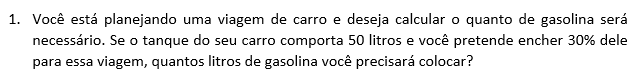
\includegraphics[width=0.85\textwidth]{questão1.png}
  \label{questão1}

  {\footnotesize Fonte: Dados da Pesquisa}
\end{figure}
\\

Na Questão 2 (Figura \ref{questão2}), os alunos serão desafiados a calcular o preço final de uma camiseta que, inicialmente, custa 80 reais, mas que está com um desconto de 20\%. Essa questão visa, principalmnte, avaliar a capacidade dos alunos de aplicar o conceito de porcentagem para determinar o valor do desconto e, em seguida, subtrair esse valor do preço original, chegando ao valor final da compra.

Esse tipo de exercício é especialmente relevante para o desenvolvimento de habilidades matemáticas aplicadas ao consumo, permitindo que os alunos compreendam como os descontos funcionam na prática e os capacitando a tomar decisões informadas em situações cotidianas de compra. Além de desenvolver o conhecimento sobre porcentagens, essa questão incentiva a autonomia na realização de cálculos financeiros básicos, contribuindo para uma formação matemática mais prática e significativa.
\\
\begin{figure}[h!]
  \centering
  \caption{Questão 2}
  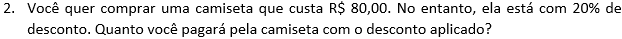
\includegraphics[width=0.85\textwidth]{questão2.png}
  \label{questão2}

  {\footnotesize Fonte: Dados da Pesquisa}
\end{figure}

Na Questão 3 (Figura \ref{questão3}), o foco está em calcular diretamente o valor economizado em uma refeição ao aplicar um desconto percentual, reforçando o entendimento da porcentagem como uma ferramenta para medir a redução de valores em contextos práticos. Através desta atividade os alunos têm a oportunidade de aplicar o conceito de porcentagem em uma situação real de consumo, consolidando sua habilidade de interpretação e cálculo de descontos.

Esse tipo de problema é essencial para desenvolver a competência dos alunos em matemática, incentivando-os a considerar a relevância financeira dos cálculos percentuais no controle de gastos e no planejamento financeiro.
\\
\begin{figure}[h!]
  \centering
  \caption{Questão 3}
  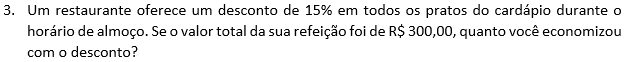
\includegraphics[width=0.85\textwidth]{questão3.png}
  \label{questão3}

  {\footnotesize Fonte: Dados da Pesquisa}
\end{figure}

Na Questão 4 (Figura \ref{questão4}), os alunos são desafiados a calcular o valor final de um par de tênis após a aplicação de um desconto percentual. O objetivo central dessa questão é verificar se os alunos aplicam o conceito de porcentagem para determinar o valor com desconto, desenvolvendo a habilidade de calcular o preço final de um item após uma redução percentual. Além disso, essa questão visa fortalecer a capacidade dos alunos de utilizar porcentagens como uma ferramenta prática para avaliar o impacto de descontos no custo final de um produto. Essa prática contribui para a formação de competências em educação financeira, incentivando os alunos a aplicarem esses conhecimentos em situações de consumo e a refletirem sobre o valor das economias obtidas.
\\
\begin{figure}[h!]
  \centering
  \caption{Questão 4}
  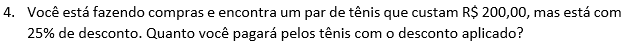
\includegraphics[width=0.85\textwidth]{questão4.png}
  \label{questão4}

  {\footnotesize Fonte: Dados da Pesquisa}
\end{figure}

Na Questão 5 (Figura \ref{questão5}), os alunos serão desafiados a calcular quantos alunos praticam esportes regularmente em uma escola com 500 alunos, considerando que 40\% deles se dedicam a essa atividade. O objetivo principal é verificar se os alunos percebem dados percentuais interpretados em cenários cotidianos, como o número de praticantes de esportes em uma escola, e aplicar a porcentagem para obter resultados quantitativos. Além disso, a questão verifica se os estudantes possuem a habilidade de compreender o significado da porcentagem como uma representação de um subconjunto dentro de uma população, uma competência essencial para a interpretação de dados em contextos variados, como saúde, educação e outras estatísticas relevantes.
\\
\begin{figure}[h!]
  \centering
  \caption{Questão 5}
  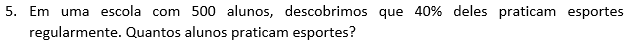
\includegraphics[width=0.85\textwidth]{questão5.png}
  \label{questão5}

  {\footnotesize Fonte: Dados da Pesquisa}
\end{figure}
\\


\subsection{Encontro 1}

No primeiro encontro, será apresentado de forma clara o objetivo do experimento e explicado sobre a importância do conceito de porcentagem no planejamento orçamentário familiar. Em seguida, deve-se explicar as metodologias a serem utilizadas ao longo do experimento: Aprendizagem Baseada em Problemas- ABP e Rotação por Estações, incluindo suas vantagens em ambientes educacionais. Nesta sessão, os participantes responderão ao Questionário 1 e farão o Pré-Teste, que constam nos Apêndices \ref{ApendiceA} e \ref{ApendiceB}.



\subsection{Encontro 2}
\label{subsec:encontro2}

Para o segundo encontro, será realizada uma aula de 3 horas, dividida em 4 tempos de 45 minutos cada, utilizando a metodologia de Rotação por Estações. A sala de aula deverá ser organizada em três grupos, e em três estações diferentes.

Após formação das equipes,  será realizada uma apresentação sobre o funcionamento da metodologia de Rotação por Estações, com explicação no quadro. Dessa forma, as equipes terão liberdade para escolher o percurso que desejam seguir durante as trocas de estações, o que favorece a integração colaborativa entre os participantes. Essa abordagem está em sintonia com as competências gerais da Educação Básica, conforme proposta pela BNCC, “Agir pessoal e coletivamente com autonomia, responsabilidade, flexibilidade, resiliência e determinação, tomando decisões com base em princípios éticos, democráticos, inclusivos, sustentáveis e solidários” (\cite{Educacao.2018},, p. 12).

Nesse momento, cada equipe também receberá sua lista de materiais, composta por uma página para registros e anotações ao longo das atividades, uma folha com instruções claras das tarefas a serem realizadas e um caderno para execução e pesquisa. Esses documentos estão disponíveis no Apêndice \ref{ApendiceC} desta dissertação.

Cada grupo participará por 1 hora em cada estação, de modo que todos os grupos passarão por todas as estações. A seguir, estão descritas as atividades que devem ser realizadas nas estações.

\\
\begin{center}
  \textbf{Estação I: Controle Orçamentário}
\end{center}
\\

Os alunos receberam a tarefa de ajustar proporcionalmente um orçamento familiar fictício, considerando um aumento na receita da família. Em seguida, precisaram reduzir o valor final em 10\%, como forma de criar uma reserva para emergências, conforme as figuras \ref{Atividade na Estação de Controle Orçamentário} e \ref{controleorçamentário} .

\\
\begin{figure}[h!]
  \centering
  \caption{Atividade na Estação I: Controle Orçamentário}
  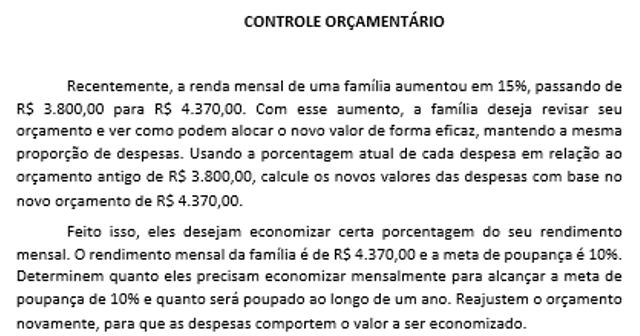
\includegraphics[width=1\textwidth]{Atividade na Estação de Controle Orçamentário.png}
  \label{Atividade na Estação de Controle Orçamentário}

  {\footnotesize Fonte: Dados da Pesquisa}
\end{figure}
\\

\\
\begin{figure}[h!]
  \centering
  \caption{Atividade na Estação I: Controle Orçamentário}
  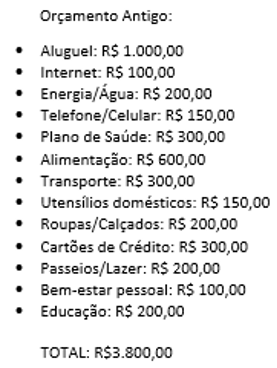
\includegraphics[width=0.45\textwidth]{controleorçamentário.png}
  \label{controleorçamentário}

  {\footnotesize Fonte: Dados da Pesquisa}
\end{figure}

Esta atividade tem como objetivo principal aplicar o conceito de porcentagem em uma revisão orçamentária, permitindo que os alunos calculem o valor atualizado das despesas com base em um aumento proporcional da renda familiar. Além disso, a atividade oferece uma oportunidade prática para que os alunos utilizem porcentagens e realizem cálculos de orçamento em um contexto familiar, fortalecendo sua compreensão sobre a importância das proporções e do planejamento financeiro na gestão eficaz dos recursos. Ao ajustar o orçamento para a redução de uma meta de poupança, os alunos também desenvolvem habilidades para tomar decisões financeiras, informar e priorizar despesas, promovendo uma visão prática da educação financeira no cotidiano.
\\
\begin{center}

  \textbf{Estação II: Otimização do Orçamento Familiar}
\end{center}
\\

Nesta estação, os alunos trabalharão com uma planilha de Excel que contém um orçamento doméstico fictício (Figura\ref{Planilha de Orçamento Familiar da Atividade}). A proposta é que calculem a porcentagem correspondente a cada despesa e, posteriormente, criem um gráfico de pizza com base nos valores percentuais calculados, conforme Figura \ref{Estação de Otimização do Orçamento Familiar}.

\\
\begin{figure}[h!]
  \centering
  \caption{Estação II: Otimização do Orçamento Familiar}
  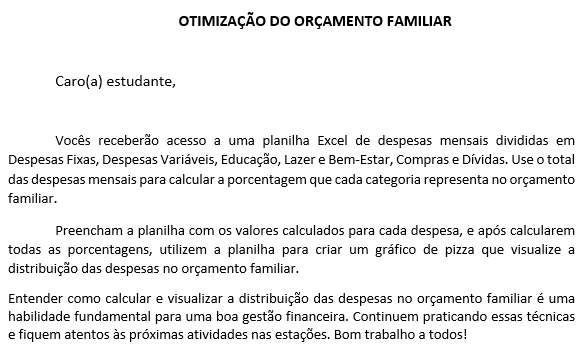
\includegraphics[width=0.9\textwidth]{Estação de Otimização do Orçamento Familiar.png}
  \label{Estação de Otimização do Orçamento Familiar}

  {\footnotesize Fonte: Dados da Pesquisa}
\end{figure}
\\
\\
\\
\begin{figure}[h!]
  \centering
  \caption{Planilha de Orçamento Familiar da Estação II}
  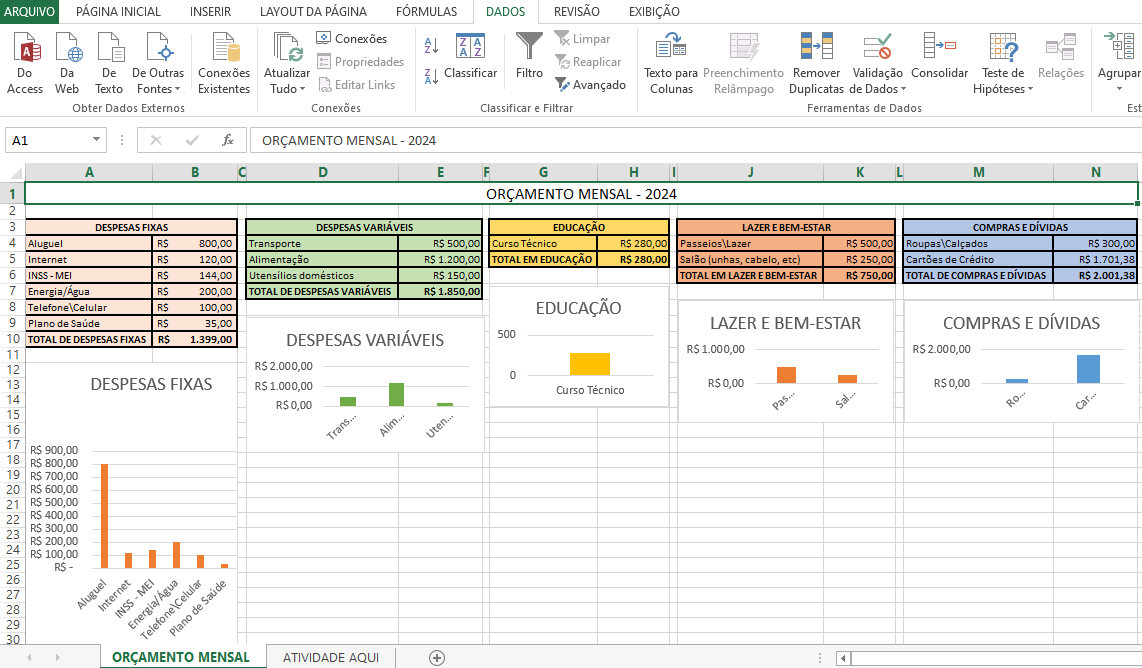
\includegraphics[width=0.9\textwidth]{Planilha de Orçamento Familiar da Atividade.png}
  \label{Planilha de Orçamento Familiar da Atividade}
  {\footnotesize Fonte: Elaboração própria}
\end{figure}
\\

Esta atividade tem como principais objetivos desenvolver habilidades de cálculo percentual aplicado, ensinando os alunos a calcular a porcentagem de cada categoria de despesa em relação ao orçamento total, além de introduzir o uso prático de planilhas eletrônicas para gestão financeira, capacitando os alunos a organizar e calcular despesas de forma autônoma em ferramentas digitais como o Excel e promover a compreensão da visualização gráfica de dados financeiros, por meio da criação de gráficos de pizza que ajudam a interpretar e analisar a distribuição das despesas.
\\
\\
\begin{center}
  \textbf{Estação III: Jogos Educativos}
\end{center}
\\

Nesta estação, os alunos se revezaram para participar de dois jogos interativos específicos para a Educação Financeira. O primeiro jogo, disponível Atividade sobre Educação Financeira - Game show de TV (wordwall.net), consiste em um quiz com 7 perguntas relacionadas ao tema Educação Financeira. Segundo Silva (\citeyear{Silva2018financeira}),
\begin{citacao}
  Os jogos educativos desempenham um papel fundamental na aprendizagem de conceitos financeiros, pois proporcionam um ambiente lúdico e interativo que facilita a compreensão e a retenção de informações. Esses jogos ajudam a desenvolver habilidades importantes, como a tomada de decisões financeiras conscientes, de forma divertida e envolvente (\cite{Silva2018financeira}p. 98).
\end{citacao}

Esse formato de quiz permite que os alunos testem seus conhecimentos de maneira dinâmica, tornando o aprendizado mais atraente e eficaz.

A pergunta 1, Figura \ref{Pergunta 1}, explora o conceito de receitas, buscando levar os alunos a entenderem a importância desse elemento no contexto financeiro. O objetivo é levar os alunos a identificar o que são receitas, ajudando-os a compreender que receitas representam os ganhos ou entradas de dinheiro, diferenciando de despesas e outros componentes financeiros. Essa distinção é fundamental para o desenvolvimento de uma visão equilibrada sobre finanças, permitindo que os alunos construam uma base sólida para o planejamento e o controle do orçamento.

A pergunta 2 aborda os passos essenciais para se elaborar um bom orçamento, conforme ilustrado na Figura \ref{Pergunta 2}. Essa questão visa não apenas ensinar aos alunos a identificar e organizar receitas e despesas, mas também desenvolver habilidades para estabelecer prioridades financeiras, capacitando-os a alocar recursos de maneira consciente e responsável. Esse conhecimento é fundamental para construir uma base sólida em planejamento financeiro.

\\
\begin{figure}[h!]
  \centering
  \caption{Pergunta 1}
  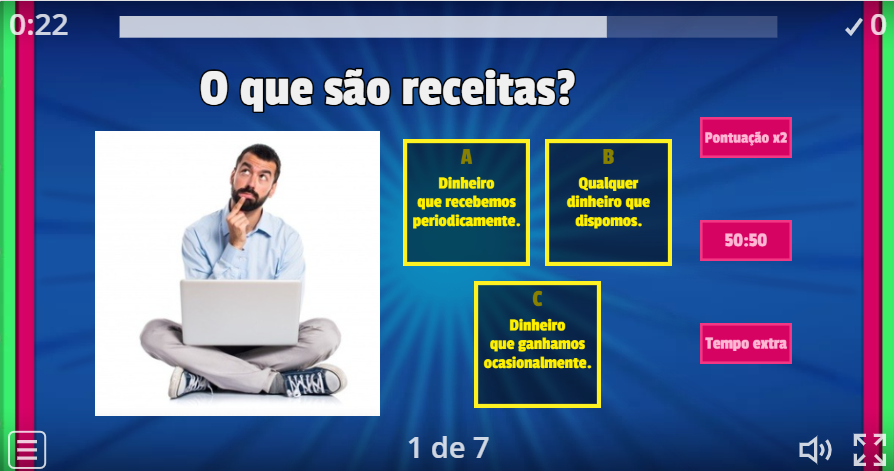
\includegraphics[width=0.85\textwidth]{Pergunta 1.png}
  \label{Pergunta 1}

  {\footnotesize Fonte:  Site do jogo}
\end{figure}

\\
\begin{figure}[h!]
  \centering
  \caption{Pergunta 2}
  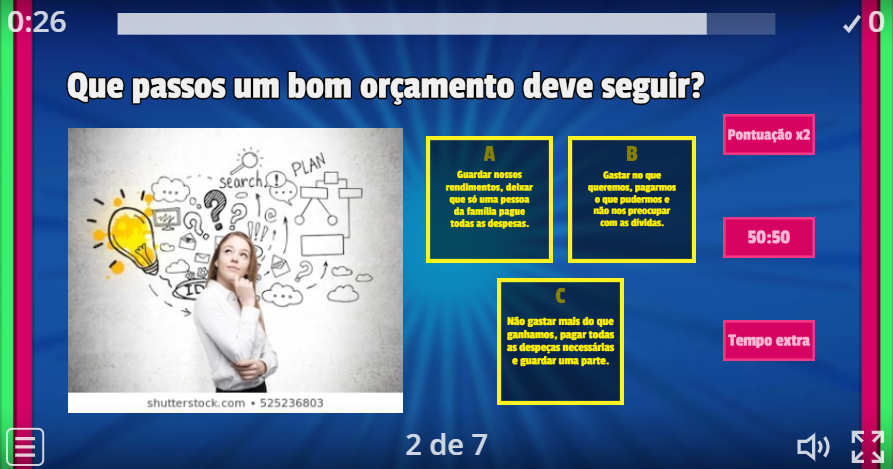
\includegraphics[width=0.85\textwidth]{Pergunta 2.png}
  \label{Pergunta 2}

  {\footnotesize Fonte:  Site do jogo}
\end{figure}

A pergunta 3, Figura \ref{Pergunta 3}, aborda a importância de um orçamento bem elaborado, que permite pagar as despesas e ainda reservar uma parte para poupança. O objetivo é levar os alunos a compreender que, ao controlar as despesas de forma eficiente, é possível destinar uma parte da renda para economia, ajudando-os a desenvolver uma mentalidade voltada para a poupança e o planejamento financeiro.

\begin{figure}[h!]
  \centering
  \caption{Pergunta 3}
  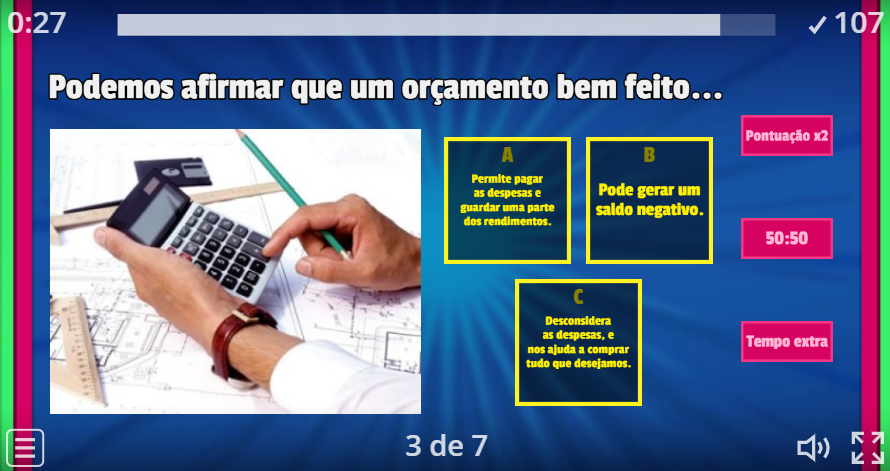
\includegraphics[width=0.85\textwidth]{Pergunta 3.png}
  \label{Pergunta 3}

  {\footnotesize Fonte:  Site do jogo}
\end{figure}

A pergunta da Figura \ref{Pergunta 4} é sobre a classificação dos produtos utilizados no dia a dia, incentivando os alunos a identificar e organizar esses produtos de acordo com suas necessidades e prioridades. O objetivo é desenvolver a habilidade de distinguir entre itens essenciais e não essenciais, promovendo uma compreensão sobre o consumo responsável e a importância de priorizar necessidades no planejamento financeiro.

\begin{figure}[h!]
  \centering
  \caption{Pergunta 4}
  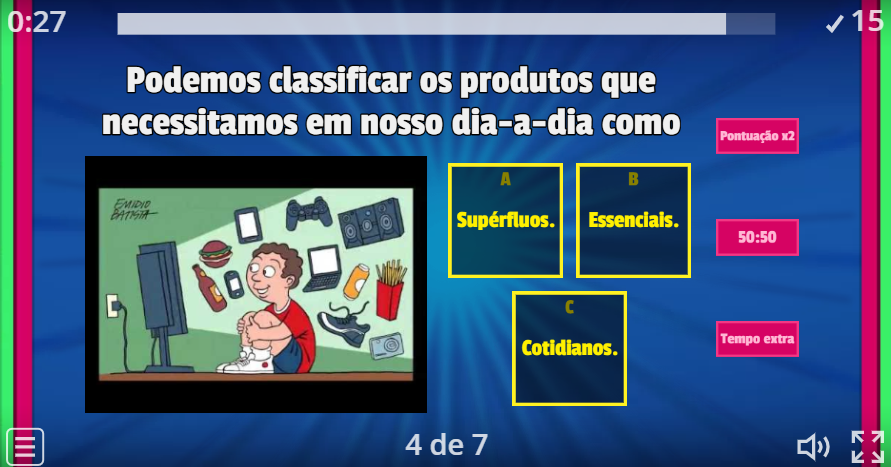
\includegraphics[width=0.85\textwidth]{Pergunta 4.png}
  \label{Pergunta 4}

  {\footnotesize Fonte:  Site do jogo}
\end{figure}

A pergunta 5, Figura \ref{Pergunta 5}, desafia os alunos a refletirem sobre o conceito de orçamento financeiro e tem como objetivo definir o que é um orçamento financeiro, desenvolvendo uma base sólida para entender a organização e o planejamento de recursos financeiros.

\begin{figure}[h!]
  \centering
  \caption{Pergunta 5}
  \includegraphics[width=0.85\textwidth]{Pergunta 5.png}
  \label{Pergunta 5}

  {\footnotesize Fonte:  Site do jogo}
\end{figure}
\\

A pergunta 6, figura \ref{Pergunta 6}, aborda o conceito de despesas, com o objetivo de ensinar aos alunos o significado desse termo no contexto financeiro. A intenção é ajudá-los a compreender que as despesas representam os gastos ou saídas de dinheiro necessárias para atender a diversas necessidades e com essa compreensão, os alunos poderão diferenciar despesas de outros componentes do orçamento, como receitas e poupança, e entender como o controle das despesas é essencial para manter o equilíbrio financeiro, são incentivados a refletir sobre o impacto de seus gastos e a importância de uma gestão consciente para uma organização financeira eficaz.

A pergunta 7, figura \ref{Pergunta 7}, aborda a importância do planejamento financeiro como uma ferramenta essencial para uma boa organização e controle dos recursos pessoais. Seu objetivo é promover a disciplina e a responsabilidade financeira, incentivando os alunos a adotarem práticas de organização e controle financeiro responsável. Ao compreenderem o valor de um planejamento estruturado, os alunos são encorajados a refletir sobre hábitos de consumo consciente, a estabelecer metas de poupança e a priorizar gastos de maneira equilibrada.
\\
\begin{figure}[h!]
  \centering
  \caption{Pergunta 6}
  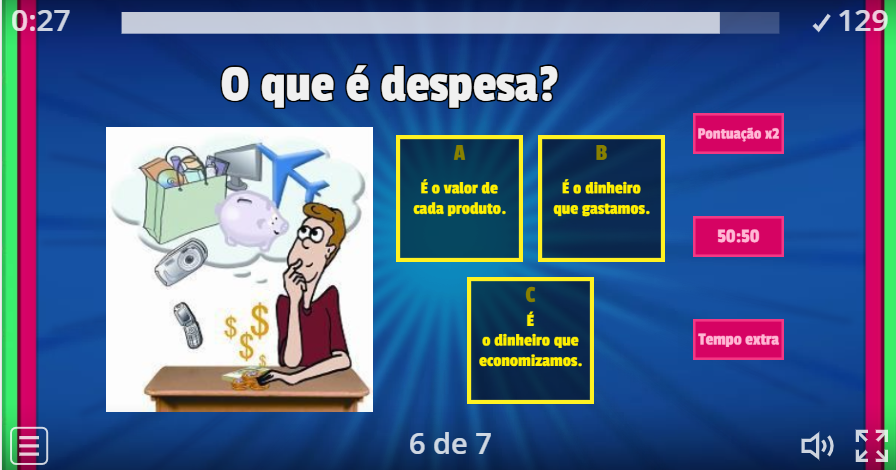
\includegraphics[width=0.85\textwidth]{Pergunta 6.png}
  \label{Pergunta 6}

  {\footnotesize Fonte:  Site do jogo}
\end{figure}
\\
\\
\begin{figure}[h!]
  \centering
  \caption{Pergunta 7}
  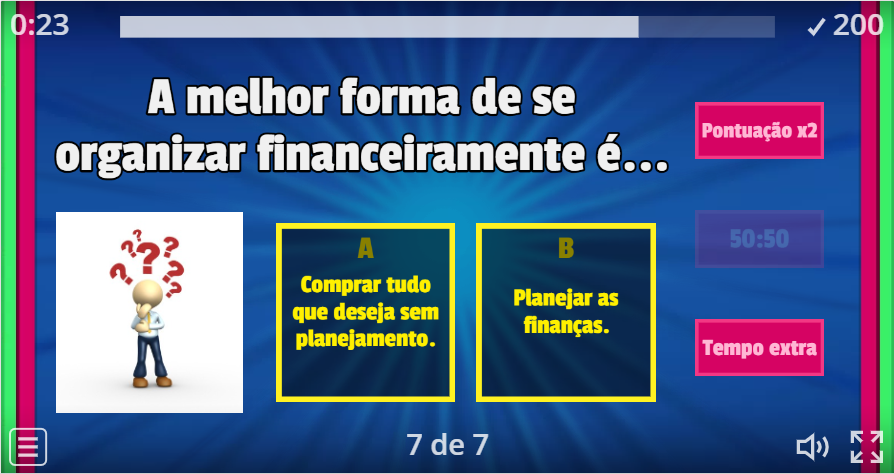
\includegraphics[width=0.85\textwidth]{Pergunta 7.png}
  \label{Pergunta 7}

  {\footnotesize Fonte:  Site do jogo}
\end{figure}
\\
\\
\\
\\

Esse jogo, também disponível em "Vamos relembrar alguns conceitosdo semestre de Ed. Financeira 5 ano - Perseguição em labirinto" \href{https://wordwall.net/pt/resource/177696/44/educa\%C3%A7%A3o-financeira-para-crian\%C3%A7as/vamos-relembrar-alguns} {, neste link}, consite em conduzir um astronauta até a resposta correta para cada pergunta relacionada à educação financeira. Esse jogo é de menor complexidade e foi pensado para incluir estudantes com necessidades educacionais especiais. Segundo Fonseca (\citeyear{Fonseca2019}),

  \begin{citacao}
    A utilização de jogos educativos no ensino de educação financeira facilita a aprendizagem, especialmente quando adaptados para incluir alunos com necessidades educacionais especiais. Esses jogos permitem uma abordagem mais dinâmica e interativa, promovendo a inclusão e o engajamento de todos os alunos no processo de aprendizagem (\cite{Fonseca2019},, p. 45).
  \end{citacao}

  O jogo é inspirado no clássico \textbf{Pac-Man}, um ícone dos videogames que alcançou grande popularidade em arcades e outras plataformas. Trata-se de uma experiência interativa e dinâmica, com uma jogabilidade simples e envolvente. A versão adaptada conta com \textbf{quatro fases}, nas quais os desafios são voltados para temas de \textbf{Educação Financeira}.

  Como supracitado, o jogador assume o controle de um personagem representado por um astronauta, que precisa escapar de extraterrestres enquanto busca resolver questões propostas em cada fase. O objetivo é analisar cuidadosamente o questionamento central e guiar o astronauta até o local onde se encontra a resposta correta.

  Na primeira fase, por exemplo, apresentada na figura \ref{Primeira pergunta} , o desafio aborda o comportamento de consumo além do necessário, incentivando os alunos a refletirem sobre as consequências desse tipo de prática no orçamento pessoal. A proposta é capacitar os jogadores a identificarem a diferença entre itens essenciais e supérfluos, desenvolvendo a habilidade de distinguir entre necessidades reais e desejos impulsivos.

  Essa compreensão é fundamental para promover uma visão mais consciente sobre o consumo, encorajando a priorização de gastos e a redução do desperdício de recursos financeiros. Com isso, o jogo não apenas transmite conhecimentos teóricos sobre Educação Financeira, mas também estimula atitudes mais responsáveis e equilibradas em relação ao uso do dinheiro, contribuindo para a formação de consumidores mais críticos e conscientes.

  \\
  \begin{figure}[h!]
    \centering
    \caption{Primeira pergunta}
    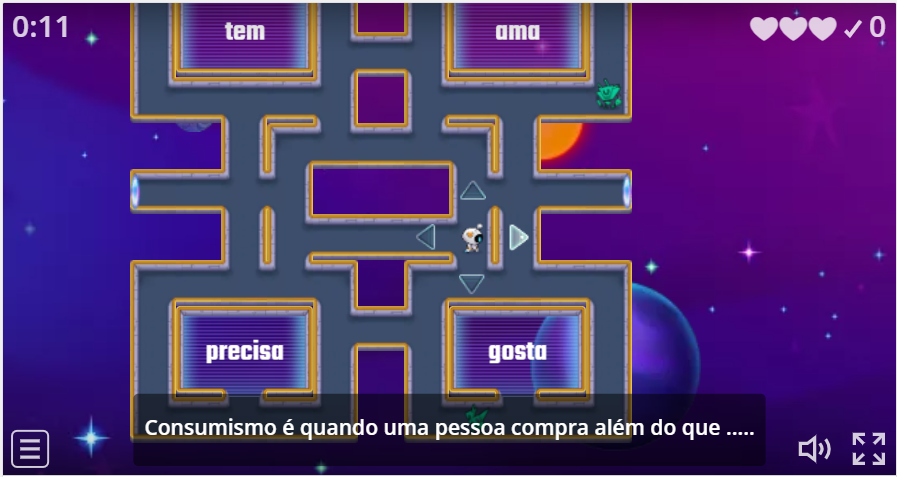
\includegraphics[width=1\textwidth]{Primeira Pergunta.png}
    \label{Primeira pergunta}
    {\footnotesize Fonte:  Site do jogo}
  \end{figure}
  \\

  A segunda fase, por exemplo, figura \ref{Segunda pergunta}, é sobre a possibilidade de atenderem desejos pessoais quando há dinheiro planejado para isso e tem como objetivo capacitar os alunos a entender a importância de equilibrar a satisfação de desejos com as obrigações financeiras e necessidades, promovendo uma gestão financeira saudável. Essa questão incentiva os alunos a refletirem sobre o uso responsável do dinheiro, mostrando que, embora seja possível realizar gastos com desejos, isso deve ser feito dentro de um planejamento que priorize as necessidades e mantenha o orçamento em equilíbrio.

  \\
  \begin{figure}[h!]
    \centering
    \caption{Segunda pergunta}
    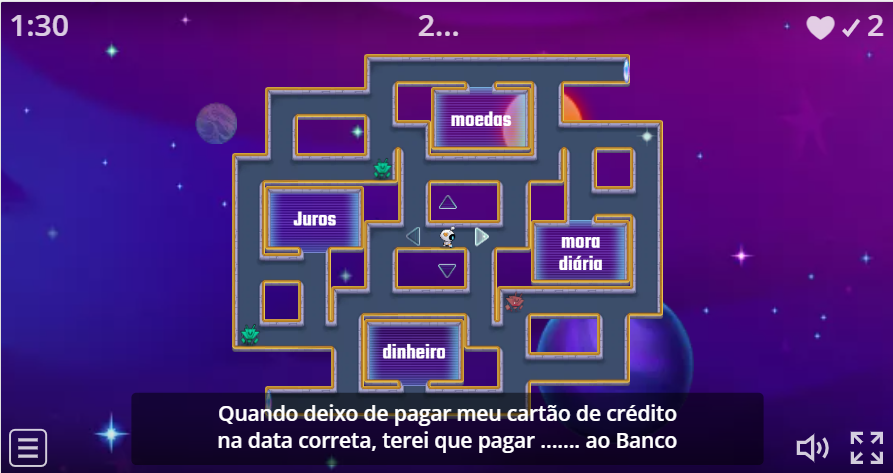
\includegraphics[width=1\textwidth]{Segunda pergunta.png}
    \label{Segunda pergunta}
    {\footnotesize Fonte:  Site do jogo}
  \end{figure}
  \\

  Essa estação não só proporciona uma abordagem lúdica ao aprendizado de conceitos financeiros, como também promove a inclusão e a diversão coletiva, com os alunos interagindo e aprendendo de forma lúdica e descontraída.





  \subsection{Encontro 3}

  No terceiro encontro serão utilizados 4 tempos de aula. Cada grupo deverá ter no máximo 10 alunos.

  Nesse encontro será apresentado o Problema 1, conforme figuras \ref{Problema 1}, \ref{Problema 1 - Gastos fixos} e \ref{Problema 1- Gastos variáveis e resumo do mês}. Os passos necessários para a realização da atividade serão expostos no quadro, e os grupos começarão a trabalhar na solução.

  O Problema 1 é sobre o planejamento financeiro familiar e a organização das finanças para a compra de um carro próprio. O Problema 1 é sobre o planejamento financeiro familiar e a organização das finanças para a compra de um carro próprio. Com essa atividade, buscamos desenvolver nos alunos a compreensão e a aplicação do conceito de porcentagem e planejamento financeiro, incentivando-os a identificar e entender os componentes do orçamento familiar, como renda, despesas fixas e variáveis, além da importância de investimentos.

  Além disso, espera-se que eles explorem o conceito de reserva de emergência, compreendendo a importância de destinar uma porcentagem da renda para emergências e refletindo sobre como os imprevistos podem afetar o planejamento financeiro da família.

  Segundo o Banco Central do Brasil (\citeyear{bancocentral_educacao_financeira}), o planejamento financeiro familiar é essencial para garantir a estabilidade econômica das famílias, permitindo que elas lidem melhor com imprevistos e alcancem seus objetivos a longo prazo, como a compra de um carro ou a construção de uma reserva financeira sólida.

  A atividade também incentiva o desenvolvimento da competência de tomada de decisão financeira, promovendo a reflexão sobre as melhores alternativas para alcançar objetivos de longo prazo e sobre o impacto das decisões financeiras na vida cotidiana. Um dos principais focos é aplicar conceitos de matemática financeira, como juros simples e compostos, para que os alunos compreendam o impacto dos juros no custo final de um bem, avaliando a diferença entre a compra à vista e o financiamento de bens.
  \\
  \begin{figure}[h!]
    \centering
    \caption{Problema 1}
    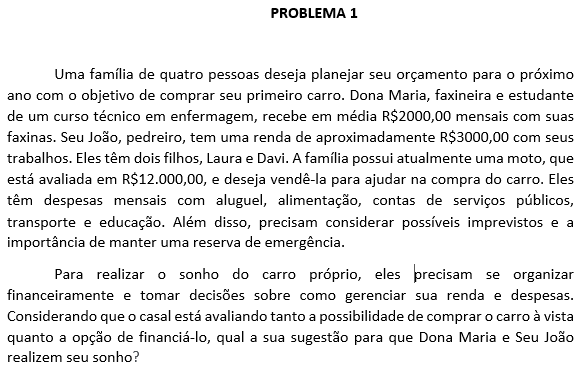
\includegraphics[width=1\textwidth]{Problema 1.png}
    \label{Problema 1}
    {\footnotesize Fonte:  Dados da Pesquisa}
  \end{figure}
  \\
  \\
  \begin{figure}[h!]
    \centering
    \caption{Problema 1 - Gastos fixos}
    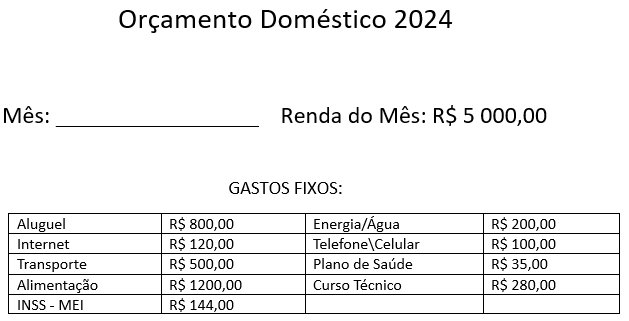
\includegraphics[width=0.8\textwidth]{Problema 1 - Gastos Fixos.png}
    \label{Problema 1 - Gastos fixos}

    {\footnotesize Fonte: Dados da Pesquisa}
  \end{figure}

  \\
  \begin{figure}[h!]
    \centering
    \caption{Problema 1- Gastos variáveis e resumo do mês}
    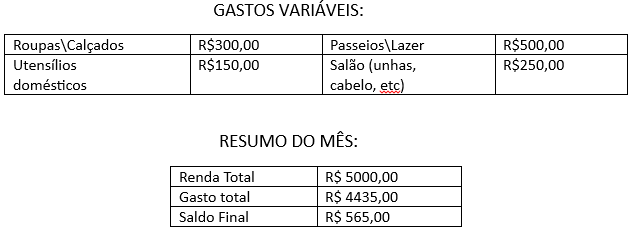
\includegraphics[width=0.8\textwidth]{Problema 1 - Gastos variáveis e resumo do mêsl.png}
    \label{Problema 1- Gastos variáveis e resumo do mês}

    {\footnotesize Fonte:  Dados da Pesquisa}
  \end{figure}

  Segundo o Sebrae (\citeyear{sebrae_educacao_financeira}),

  \begin{citacao}
    A educação financeira é uma ferramenta indispensável para a formação de cidadãos conscientes e preparados para os desafios da vida adulta. Inserir esse tema nas salas de aula possibilita aos alunos o desenvolvimento de habilidades essenciais, como o planejamento financeiro, a economia consciente e o entendimento de investimentos (\cite{sebrae_educacao_financeira})).
  \end{citacao}

  No que se refira à porcentagem, a atividade permite que os alunos compreendam e apliquem cálculos percentuais em situações do cotidiano, como a porcentagem da renda que uma família poderia poupar mensalmente. Ao simular a compra do carro, os alunos são incentivados a comparar as opções de compra à vista e de financiamento usando cálculos percentuais, analisando o valor adicional que o financiamento representa em relação ao custo total do carro. Segundo Siqueira e Lopes (\citeyear{siqueira2020matematica}),

  \begin{citacao}
    A implementação de atividades práticas que envolvem cálculos percentuais permite aos alunos desenvolverem uma compreensão mais aprofundada sobre a importância da matemática financeira no cotidiano. Essas atividades não apenas ajudam na assimilação de conceitos teóricos, mas também incentivam os estudantes a refletirem sobre a aplicação desses conceitos em decisões financeiras reais (\cite{siqueira2020matematica},, p. 89).
  \end{citacao}
  \\

  Além disso, eles são levados a calcular a aplicação de juros compostos em financiamentos, projetando o custo adicional ao longo do tempo e a porcentagem que esses juros representam sobre o valor inicial do bem. Essa abordagem integrada ajuda os alunos a aplicar conceitos matemáticos e financeiros em contextos reais, promovendo uma visão mais prática e consciente do uso do dinheiro e das implicações das decisões financeiras para a realização de metas e objetivos.

  Para realizar as atividades, os alunos devem seguir os seguintes passos, utilizando a ABP:

  \begin{enumerate}


    \item Esclarecimento de Termos e Conceitos:

          O objetivo é que os alunos esclareçam
          os termos e conceitos fundamentais envolvidos no planejamento financeiro da família. Eles discutem termos como orçamento, renda, despesas fixas e variáveis, reserva de emergência, financiamento e porcentagem. Nessa etapa, os alunos se organizam e, com uma lista de termos relacionados ao planejamento financeiro, pesquisam e discutem o significado dos conceitos, utilizando exemplos práticos para tornar o entendimento mais claro. Ao final, analisamos suas definições e discutimos com a turma, promovendo uma construção colaborativa do conhecimento e permitindo que todos compreendam os vocabulários essenciais para formular soluções viáveis e realistas para o problema.
          \\
    \item Definição do Problema:

          Os alunos trabalham na definição do problema central, que é como uma família pode se organizar financeiramente para realizar o sonho de comprar um carro, considerando as fontes de renda, as despesas e a importância de uma reserva de emergência. Eles precisam entender os objetivos e desafios da família, e, para isso, discutir o problema da maneira mais completa possível, destacando elementos- chave, como o sonho de comprar o carro, o orçamento familiar, a possibilidade de vender a moto e os fatores que influenciam a decisão, como os juros do financiamento e a necessidade de economia. Ao realizar esta análise, os alunos desenvolvem uma visão clara do problema que precisam resolver, identificando todos os elementos essenciais e refletindo sobre a importância prática do planejamento financeiro.
          \\
    \item Análise do Problema:

          Os alunos analisam detalhadamente o problema e
          começam a identificar dados concretos, como as fontes de renda e os tipos de despesas da família. Essa análise envolve levantar os dados financeiros da família, incluindo a renda de Dona Maria e Seu João, o valor da moto e as despesas monetárias, além de categorizar essas despesas em fixas e variáveis. A partir desses dados, os alunos calculam o saldo mensal da família e projetam o valor necessário para uma reserva de emergência, definindo uma porcentagem viável da renda mensal que pode ser destinada a essa especificidade. Essa etapa permite que os alunos aprofundem seu entendimento sobre o problema e desenvolvam a habilidade de categorização, essenciais para a tomada de decisões, ao aprender a analisar a situação financeira e definir limites que orientarão o planejamento.
          \\
    \item Formulação de Hipóteses:

          Os alunos formulam hipóteses sobre possíveis soluções para o problema, considerando diferentes cenários que podem ajudar a família a alcançar o objetivo de comprar o carro. Nesse ponto, eles refletem sobre alternativas, como poupar uma porcentagem da renda mensal, vender uma moto para agregar mais recursos ou optar pelo financiamento do carro. Eles elaboram hipóteses e analisam o impacto de cada um no orçamento familiar. Por exemplo, podem levantar a hipótese de que, se uma família economizar 15\% da renda mensal e vender uma moto, será possível comprar o carro à vista em determinado número de meses. Esse processo ajuda a desenvolver o pensamento crítico e a capacidade de criar soluções alternativas, permitindo que os alunos compreendam como as decisões financeiras podem afetar o orçamento a longo prazo e incentivando-os a equilibrar diferentes fatores, como
          economias, juros e imprevistos.
  \end{enumerate}



  \subsection{Encontro 4}

  Para o Encontro 4 deverão ser utilizadas 4 aulas para a realização das atividades, dando continuação à sequência.

  \begin{enumerate}[start=5]
    \item  Estudo Independente:

          Os alunos se dedicam à pesquisa e ao aprofundamento dos conhecimentos necessários para avaliar as hipóteses levantadas no Passo 4. Nesta etapa, cada aluno ou grupo investiga temas específicos que são fundamentais para a solução do problema, como cálculos de porcentagem, o funcionamento de juros simples e compostos, a análise de vantagens e desvantagens entre financiamento e compras à vista, além de boas práticas de economia familiar.  O estudo independente é essencial para que os alunos adquiram uma compreensão mais sólida e crítica das informações antes de propor soluções definitivas. Eles buscam fontes como artigos, livros e simuladores financeiros, e também podem trabalhar em cálculos aplicados à situação financeira da família, como calcular o valor final de um carro financiado em comparação com a compra à vista ou o impacto de economia de uma porcentagem específica da renda ao longo do ano. Esse estudo ajuda a consolidar o conhecimento e traz segurança para os alunos ao lidarem com questões financeiras complexas.
          \\
    \item Discussão das Hipóteses e Tomada de Decisão:

          Os alunos retornam ao grupo para compartilhar o que aprenderam e aplicar esse conhecimento às hipóteses formuladas anteriormente. Discutem as informações obtidas e analisam as hipóteses com base em dados e novos conhecimentos. Nesse momento, os alunos devem avaliar quais das hipóteses são mais viáveis para a situação da família, considerando fatores como custos totais, impacto no orçamento mensal e o tempo necessário para realizar a compra do carro. Com o apoio de seus pares e orientados pelo professor, eles discutem as vantagens e especificações de cada hipótese e utilizam cálculos específicos, como porcentagem e juros, para comparar as opções. Ao final da discussão, o grupo escolhe uma solução que considera a mais adequada, levando em conta todos os fatores e o objetivo da família. Este passo fomenta a tomada de decisão colaborativa e ajuda os alunos a perceber que, em problemas reais, é necessário ponderar diferentes aspectos antes de chegar a uma solução.
          \\
    \item Apresentação da Solução:

          O grupo formaliza a solução escolhida e prepara uma apresentação para compartilhá-la com os colegas e o professor. Durante a apresentação, eles explicam o cálculo por trás de sua escolha, os cálculos realizados e os dados encontrados, mostrando por que consideraram essa solução a mais viável para a compra do carro da família. Esta apresentação permite que os grupos demonstrem as estratégias de economia propostas, justifiquem a opção de financiar ou comprar à vista e expliquem o impacto dessa decisão no orçamento familiar. Ao final, eles recebem feedback dos colegas e do professor, que podem sugerir ajustes ou dicas novas para aprimorar a solução apresentada. Essa etapa desenvolve habilidades de comunicação e organização, permitindo que os alunos defendam suas ideias com embasamento e revisem seus pontos de vista com base nas reclamações recebidas. Essa apresentação final também oferece uma oportunidade para que todos compartilhem lições sobre planejamento financeiro, consolidando a compreensão do tema e valorizando o trabalho em equipe na resolução de problemas.
  \end{enumerate}

  \subsection{Encontro 5}

  No encontro 5 os alunos deverão realizar uma prova para avaliar os conhecimentos adquiridos ao longo do processo e responder ao Questionário 2 e Questionário 3 (Apêndices F e G). O objetivo desta etapa é verificar o quanto os alunos aprenderam e aplicaram as habilidades adquiridas durante os encontros anteriores, consolidando o aprendizado.

  Para esse encontro, devem ser utilizados 2 tempos de aula. A avaliação de conhecimentos adquiridos (Pós-Teste), Apêndice H, foi elaborada com base no teste de conhecimentos prévios, com questões semelhantes. Esse formato foi adotado para permitir uma comparação precisa entre os resultados antes e após a aplicação da pesquisa, proporcionando uma análise clara do progresso dos alunos ao longo do processo.

  Os questionários 2 e 3, cada um com dez perguntas, foram elaborados com o objetivo de captar detalhadamente a percepção dos alunos sobre as metodologias Rotação por Estações e ABP, que foram aplicadas ao longo do processo de aprendizagem (Apêndices F e G). Cada pergunta é estruturada como uma afirmação fechada, permitindo aos alunos expressarem suas opiniões de forma objetiva sobre diferentes aspectos dessas metodologias. Através dessas afirmações, busca-se avaliar se os alunos consideram que:
  \begin{enumerate}[label=\roman*]
    \item- as metodologias usadas já eram conhecidas por eles;
    \item- são eficazes;
    \item- promovem um aprendizado mais profundo e significativo;
    \item- são importantes para
          preparar os alunos para enfrentarem os desafios do mundo real;
    \item- podem aumentar o envolvimento dos alunos nas atividades de aprendizagem;
    \item- desenvolvem habilidade de resolução de problemas de forma mais eficaz;
    \item- ajudam os alunos a desenvolverem habilidades de trabalho em equipe;
    \item- ajudam os alunos a desenvolverem habilidades
          de autogestão.
  \end{enumerate}

  Essas perguntas buscam oferecer uma visão abrangente sobre como os alunos experienciam e respondem a essas metodologias, permitindo uma análise específica de sua eficácia e impacto no processo de ensino-aprendizagem.

  %Os alunos realizaram novas pesquisas na internet e visitaram o site \url{https://www.calcule.net/financeiro/simulador-de-financiamento-de-veiculos-simulacao-online/#google_vignette} , que oferece simulações com as taxas de juros de diversos bancos, 
  %DEIXEI ESSE PARÁGRAFO PORQUE AQUI O LINK FICOU AJUSTADO NO TEXTO. 

  \chapter{Experimentação e análise de dados}

  Neste capítulo, serão discutidos os resultados das análises realizadas a partir das atividades de registro dos alunos e das observações da pesquisadora durante o desenvolvimento do estudo.  Essas análises desempenham um papel crucial na pesquisa, trazendo insights avançados sobre o avanço dos alunos e o impacto das estratégias de ensino aplicadas.

  Para a implementação da Sequência Didática na turma de EJA, foi selecionada uma turma mista do Ensino Fundamental II, da Escola Estadual Municipalizada Victor Sence, localizada em Conceição de Macabu, Rio de Janeiro. A escolha dessa turma se deu pela facilidade da professora pesquisadora, que atua como regente na instituição, em organizar os encontros previstos na pesquisa.

  Durante o primeiro encontro, compareceram 8 alunos; no segundo, 12; no terceiro, 10; no quarto, 8; e no último, 10 alunos. Assim, 7 alunos foram presentes em todos os encontros, e somente eles serão incluídos na análise dos dados. Esses alunos foram identificados como alunos 1, 2, 3... até o 7, mantendo essa numeração em toda a análise de dados, de modo que, por exemplo, o aluno 1 se refira à mesma pessoa em todas as etapas do estudo.




  \section{Análise do Questionário Investigativo}

  A princípio, a pesquisadora chamou a turma para participar da pesquisa, explicando a organização do trabalho, o tema a ser abordado e os objetivos do estudo. Além disso, ela esclareceu que os dados serão analisados, tornando necessária a autorização dos alunos para participarem.

  Foi então disponibilizado um termo de autorização para assinatura dos alunos. É importante ressaltar que todos os alunos assinaram, o que possibilitou a análise dos dados de todos os presentes.

  Após isso, os alunos receberam o Questionário 1 (Apêndice \ref{ApendiceA}) e o Teste de Conhecimentos Prévios (\ref{ApendiceB}), a serem respondidos individualmente com base no conhecimento que já possuíam sobre o tema de porcentagem (Figura \ref{alunos Respondendo ao Teste de Conhecimentos Prévios Sobre Porcentagem}).


  \\
  \begin{figure}[h!]
    \centering
    \caption{Alunos Respondendo ao Teste de Conhecimentos Prévios Sobre Porcentagem}
    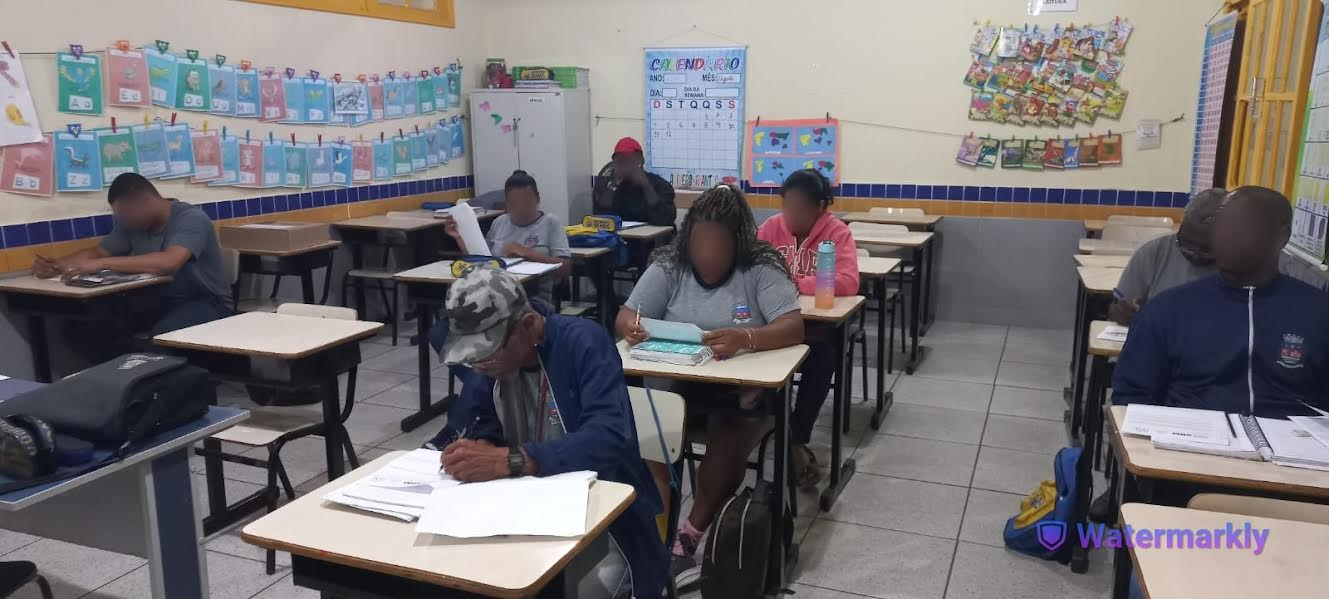
\includegraphics[width=0.85\textwidth]{Alunos respondendo conhecimentos previos porcentagem.jpg}
    \label{alunos Respondendo ao Teste de Conhecimentos Prévios Sobre Porcentagem}

    {\footnotesize Fonte:  Dados da Pesquisa}
  \end{figure}
  \\

  No início, alguns alunos demonstraram resistência em realizar as atividades, mencionando preocupações sobre não se lembrarem de certos conceitos relacionados a porcentagem. Contudo, após uma segunda conversa com a turma, em que foi esclarecido que os resultados não continham caráter avaliativo, mas sim o propósito de contribuir para a pesquisa, os alunos demonstraram maior disposição para colaborar na experimentação.

  O questionário inicial revelou que a pesquisa foi conduzida por alunos entre 17 e 80 anos, com predominância de participantes do gênero feminino (Figura \ref{idade e genero}).

  \begin{figure}[h]
    \centering
    \caption{Dados em Relação a Idade e Sexo dos Alunos}
    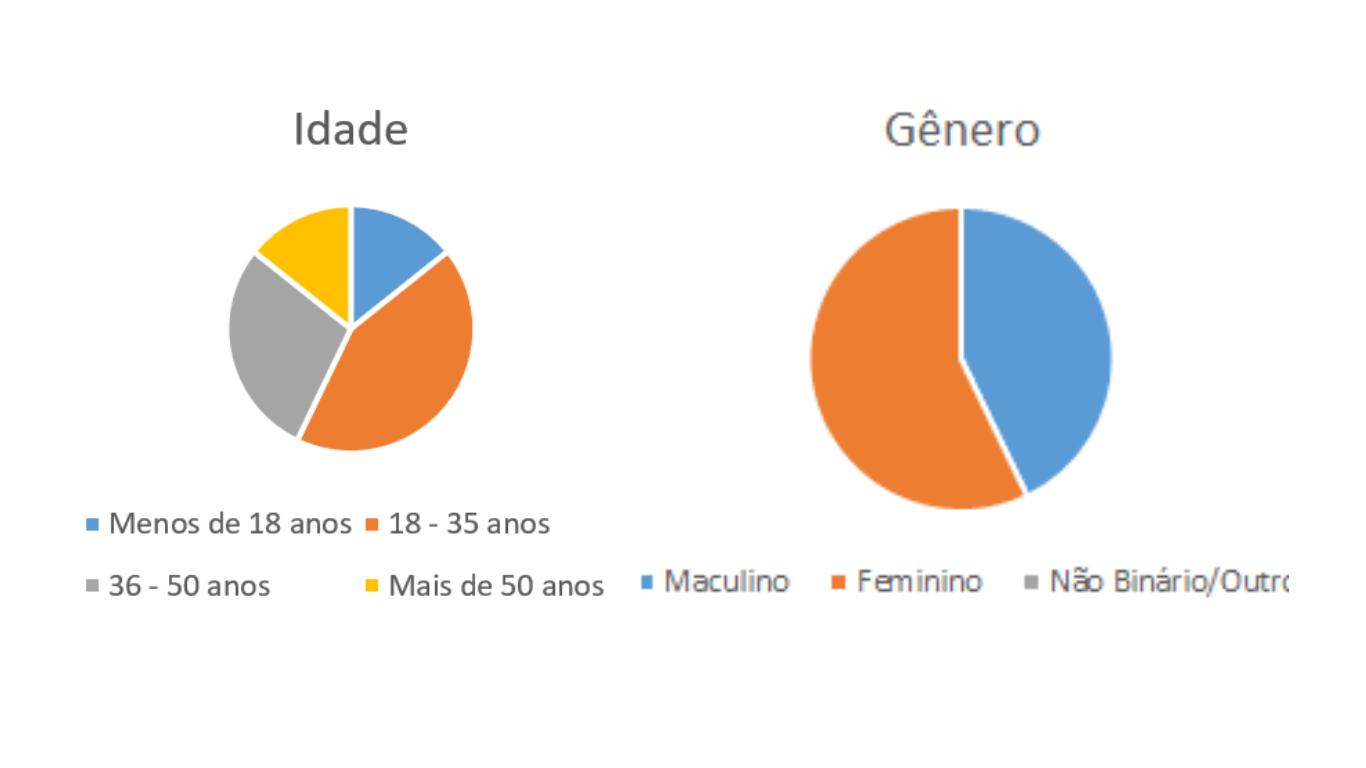
\includegraphics[width=0.75\textwidth]{Idade e genero.png}
    \label{idade e genero}

    {\footnotesize Fonte:  Dados da Pesquisa}
  \end{figure}

  \\



  Observe-se que uma grande parte dos alunos considera ter conhecimentos básicos de educação financeira, envolvendo noções como planejamento, controle de despesas e poupança, o que sugere uma familiaridade inicial com o tema (Figura \ref{dados em relação ao conhecimento previo de porcentagem} ).
  \\
  \begin{figure}[h!]
    \centering
    \caption{Dados em Relação ao Conhecimento Prévio Sobre Conceitos Básicos de Educação Financeira
    }
    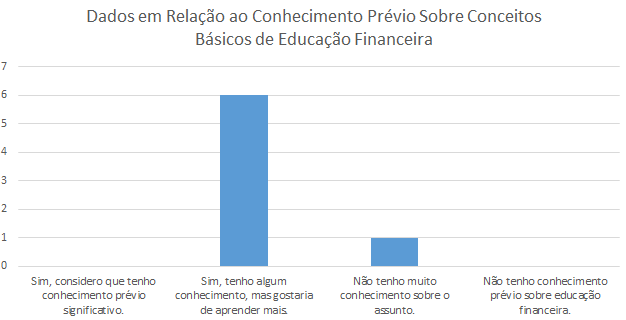
\includegraphics[width=0.8\textwidth]{Dados em Relação ao Conhecimento Prévio Sobre Conceitos Básicos de Educação Financeira.png}
    \label{dados em relação ao conhecimento previo de porcentagem}

    {\footnotesize Fonte:  Dados da Pesquisa}
  \end{figure}
  \\


  Conforme destacado no "Caderno de Educação Financeira – Gestão de Finanças Pessoais" do Banco Central do Brasil: “Todo cidadão pode desenvolver habilidades para melhorar sua qualidade de vida e de seus familiares, a partir de atitudes comportamentais e de conhecimentos básicos sobre gestão de finanças pessoais aplicadas no seu dia a dia” (\cite{bancocentral2013_educacao_financeira},, p. 3).

  A maioria dos alunos indicou possuir um nível moderado de habilidade para lidar com questões financeiras, Figura \ref{nivel de confiança}, o que sugere uma familiaridade básica, mas não totalmente aprofundada, com o tema.

  Quanto à percepção dos alunos sobre a relevância da educação financeira no cotidiano, conforme ilustrado na Figura \ref{importancia da educação financeira}, incluindo seu entendimento de como esses conhecimentos podem impactar suas vidas ao auxiliar na tomada de decisões, no planejamento futuro e na segurança dos recursos administrados, a maioria respondeu que considera essa habilidade muito importante para o desenvolvimento pessoal e profissional. Conforme destacado por Sarmento (\citeyear{Sarmento2021}):

  \begin{citacao}
    O intuito da educação financeira não se limita somente a ajudar as pessoas na tarefa de administrar o dinheiro simplesmente por administrar. Ela permite que todos tenham mais conhecimento e consciência sobre as próprias receitas e despesas, mais confiança para investir, cuidem do futuro proporcionando a segurança prevenção de problemas para que as dificuldades não sejam aplicadas. Além disso, traz melhorias nas relações pessoais e profissionais e, por conseguinte, paz de espírito e uma saúde financeira equilibrada (\cite{Sarmento2021},, p. 2).
  \end{citacao}
  \\
  \begin{figure}[h!]
    \centering
    \caption{Nível de Confiança em Lidar Com Questões Financeiras
    }
    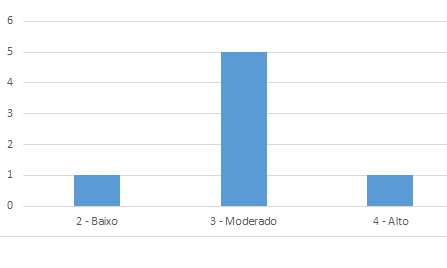
\includegraphics[width=0.85\textwidth]{Nivel de confiança.png}
    \label{nivel de confiança}

    {\footnotesize Fonte:  Dados da Pesquisa}
  \end{figure}
  \\
  \\
  \begin{figure}[h!]
    \centering
    \caption{Importância de Aprender sobre Educação Financeira
    }
    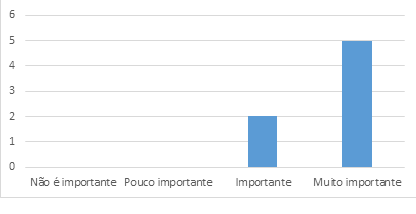
\includegraphics[width=0.85\textwidth]{importancia da educação financeira.png}
    \label{importancia da educação financeira}


    {\footnotesize Fonte:  Dados da Pesquisa}
  \end{figure}

  Quanto à frequência e ao nível de contato dos alunos com situações de gerenciamento de recursos, como compras, pagamentos, orçamento pessoal e economias, as respostas mostraram grande diversidade, conforme Figura \ref{experiencia em lhe dar com dinheiro}. A maioria dos alunos indicou experiências em "muitas vezes" ou "poucas vezes" ao lidar com dinheiro e tomar decisões financeiras.
  \\
  \begin{figure}[h!]
    \centering
    \caption{Frequência que os Alunos Tiveram Experiências em Lidar Com Dinheiro ou Fazer Escolhas Financeiras
    }
    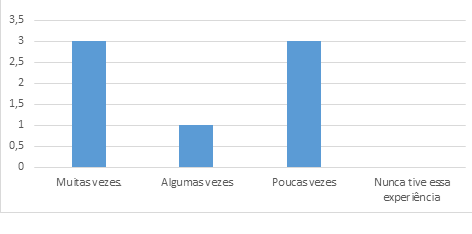
\includegraphics[width=0.85\textwidth]{experiencia em lhe dar com dinheiro.png}
    \label{experiencia em lhe dar com dinheiro}


    {\footnotesize Fonte:  Dados da Pesquisa}
  \end{figure}

  Em relação à compreensão dos alunos sobre o conceito de orçamento doméstico e sua importância, incluindo o entendimento de como ele contribui para o controle financeiro familiar, gestão eficiente dos recursos, planejamento de despesas e economia para alcançar objetivos, a maioria respondeu que conhecia o conceito e é considerado essencial para uma organização financeira adequada, conforme a Figura \ref{gráfico o que é orçamento}.

  \begin{figure}[h!]
    \centering
    \caption{Gráfico Sobre a Compreensão do Que é Orçamento Doméstico e Sua Importância
    }
    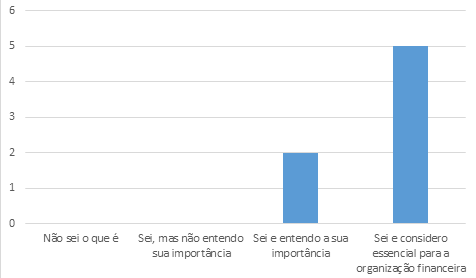
\includegraphics[width=0.85\textwidth]{grafico o que é orçamento.png}
    \label{gráfico o que é orçamento}

    {\footnotesize Fonte:  Dados da Pesquisa}
  \end{figure}

  À respeito do conhecimento dos alunos sobre as despesas regulares que compõem seu orçamento doméstico — como contas de água, luz, alimentação, aluguel, transporte, entre outros, essenciais para o controle financeiro — a maioria indicou gastos com alimentação, transporte e cuidados pessoais. Vale destacar que a pergunta permite selecionar múltiplas opções de resposta, o que reforça a percepção dos alunos sobre esses itens como parte central de seu orçamento, conforme a Figura \ref{despesas regulares}.
  \\
  \begin{figure}[h!]
    \centering
    \caption{Despesas Regulares  no Orçamento Doméstico dos Alunos
    }
    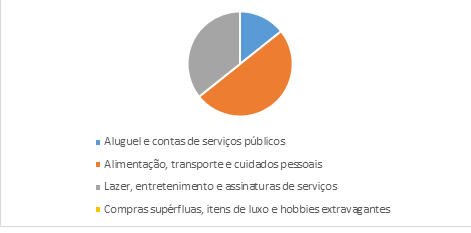
\includegraphics[width=0.85\textwidth]{despesas regulares.png}
    \label{despesas regulares}

    {\footnotesize Fonte:  Dados da Pesquisa}
  \end{figure}

  No que diz respeito a investigar se os alunos já enfrentaram dificuldades para controlar seus gastos financeiros e compreender os desafios que enfrentam ao gerenciar suas despesas dentro do orçamento, a maioria dos alunos respondeu afirmativamente, como pode ser visto na Figura \ref{dificuldade em controlar gastos}.

  \\
  \begin{figure}[h!]
    \centering
    \caption{Dificuldades em Controlar Gastos Financeiros
    }
    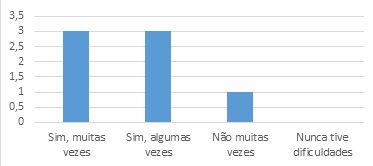
\includegraphics[width=0.85\textwidth]{dificuldade em controlar gastos.png}
    \label{dificuldade em controlar gastos}

    {\footnotesize Fonte: Dados da Pesquisa}
  \end{figure}
  \\

  Essa constatação está alinhada com os dados apresentados por Souza et al. (\citeyear{souza2022desafios}), que destaca:

  \begin{citacao}
    Os indicadores econômicos apresentam crescimento do endividamento das famílias brasileiras, apesar dos programas de Educação Financeira apoiados pelo Governo Federal e Mercado Financeiro, o que torna necessária uma reflexão sobre a eficácia da execução desses programas” (\cite{souza2022desafios},, p. 162).
  \end{citacao}
  \\

  A respeito do conceito de meta financeira e se os alunos já estabeleceram anteriormente, as respostas foram variadas, com predominância daqueles que afirmaram não saber o que é uma meta financeira (Figura \ref{o que é meta}).
  \\
  \begin{figure}[h!]
    \centering
    \caption{Pergunta Sobre o Conhecimento do Que é Meta Financeira e Se Já Estabeleceu Alguma Antes
    }
    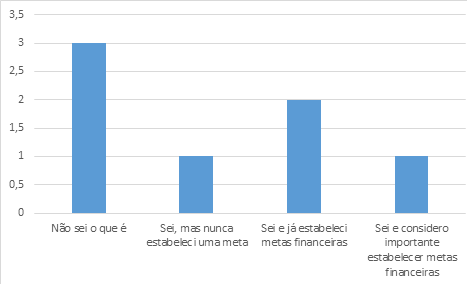
\includegraphics[width=0.85\textwidth]{o que é meta.png}
    \label{o que é meta}

    {\footnotesize Fonte:  Dados da Pesquisa}
  \end{figure}

  Uma análise das respostas dos alunos sobre como a educação financeira pode ajudar as pessoas a alcançarem seus objetivos revela uma ampla variação de opiniões, que vão desde "não pode" até "pode ajudar muito" (Figura \ref{pergunta sobre como a educação fincaneira pode auxiliar}). Esse contraste demonstra diferentes níveis de compreensão e valorização do tema, refletindo percepções que variam da desconfiança à expectativa de um impacto positivo.

  Quanto aos benefícios que os alunos associam à prática de economizar dinheiro, conforme ilustrado na Figura \ref{beneficios de economizar}, a maioria respondeu que enxerga diversas vantagens em manter uma reserva financeira. Esse entendimento demonstra que muitos alunos valorizam o ato de economia como uma estratégia para garantir a segurança financeira e alcançar metas futuras.

  Vieira e Sousa (\citeyear{vieira2020percepcao}) destacam que a conscientização sobre a importância da economia está frequentemente vinculada a experiências pessoais e ao ambiente em que o indivíduo está inserido, reforçando o papel essencial do planejamento financeiro no desenvolvimento de atitudes responsáveis em relação aos recursos financeiros.
  \\
  \begin{figure}[h!]
    \centering
    \caption{Sobre a Percepção dos Alunos de Como a Educação Financeira Pode Auxiliar as Pessoas a Atingirem Seus Objetivos
    }
    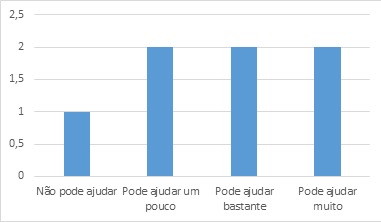
\includegraphics[width=0.85\textwidth]{pergunta sobre como educação fincanceira pode auxiliar.png}
    \label{pergunta sobre como a educação fincaneira pode auxiliar}

    {\footnotesize Fonte:  Dados da Pesquisa}
  \end{figure}
  \\

  \begin{figure}[h!]
    \centering
    \caption{Como os Alunos Enxergam os Benefícios Atribuídos à Prática de Economizar Dinheiro
    }
    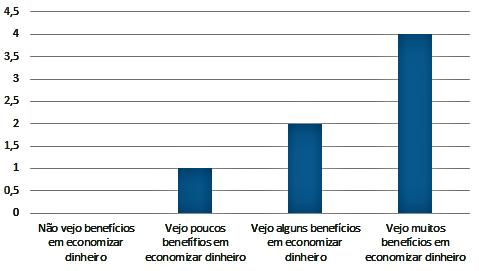
\includegraphics[width=0.85\textwidth]{Benefícios de economizar.png}
    \label{beneficios de economizar}

    {\footnotesize Fonte:  Dados da Pesquisa}
  \end{figure}
  \\

  Em relação à compreensão dos alunos sobre o conceito de consumo consciente, a importância que atribuem a ele em suas vidas e se entendem o consumo consciente como uma prática de consumo responsável — considerando o impacto ambiental, social e econômico de suas escolhas —, as respostas foram bastante variadas. Elas variaram desde \textit{"Não sei o que é"} até \textit{"Sei e considero essencial para um estilo de vida sustentável"}, refletindo diferentes níveis de consciência e valorização da sustentabilidade entre os alunos, como pode ser visto na Figura \ref{consumo consciente}.
  \\
  \begin{figure}[h!]
    \centering
    \caption{Se os Alunos Sabem a Definição e Importância do Consumo Consciente em Suas Vidas
    }
    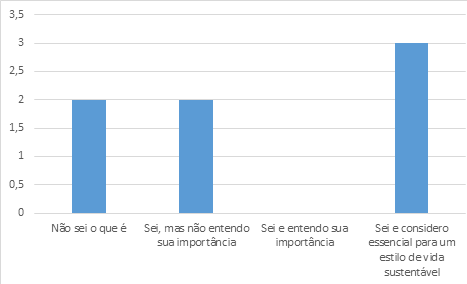
\includegraphics[width=0.85\textwidth]{consumo consciente.png}
    \label{consumo consciente}

    {\footnotesize Fonte:  Dados da Pesquisa}
  \end{figure}
  \\

  Em relação às habilidades e conhecimentos que os alunos adquirem ao estudar educação financeira, a maioria expressa o desejo de aprender uma variedade de competências. Essa expectativa indica um interesse em desenvolver habilidades práticas e ampliar seu entendimento sobre finanças, mostrando que os alunos veem valor no aprendizado financeiro para melhorar a gestão de suas próprias vidas econômicas, como pode ser visto na Figura \ref{habilidades em educação financeira}.

  Em relação ao nível de compreensão dos alunos sobre o conceito de porcentagem, Figura \ref{compreensão sobre porcentagem}, a maioria afirmou ter entendimento básico do tema. Isso mostra que, embora possuam uma noção inicial, ainda precisam de aprofundamento para aplicar o conceito de forma mais prática e abrangente em situações cotidianas.
  \\
  \\
  \begin{figure}[h!]
    \centering
    \caption{Habilidades ou Conhecimentos Que o Aluno Espera Adquirir ao Aprender Sobre Educação Financeira
    }
    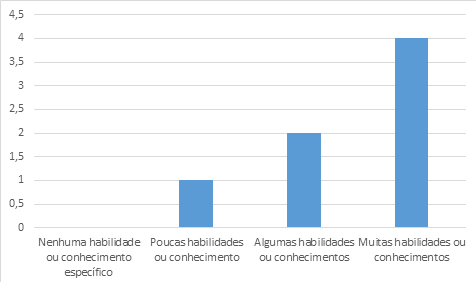
\includegraphics[width=0.85\textwidth]{habilidades em educação finceira.png}
    \label{habilidades em educação financeira}

    {\footnotesize Fonte:  Dados da Pesquisa}
  \end{figure}
  \\
  \\
  \begin{figure}[h!]
    \centering
    \caption{Nível de Compreensão dos Alunos Sobre Porcentagem
    }
    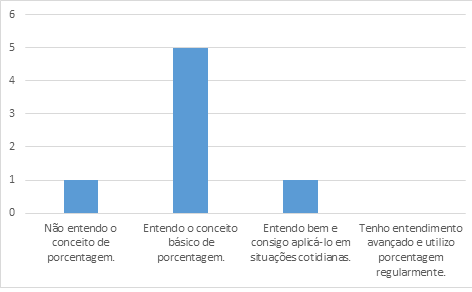
\includegraphics[width=0.85\textwidth]{compreensão sobre porcentagem.png}
    \label{compreensão sobre porcentagem}

    {\footnotesize Fonte:  Dados da Pesquisa}
  \end{figure}

  Quanto à frequência com que os alunos utilizam porcentagem em suas atividades diárias, como calcular juros e descontos, conforme ilustrado na Figura \ref{frequencia em que os alunos utilizam porcentagem},  as respostas foram variadas, com a predominância da opção "raramente."
  \\
  \begin{figure}[h!]
    \centering
    \caption{Frequência em Que os Alunos Utilizam Porcentagem em Suas Atividades Diárias
    }
    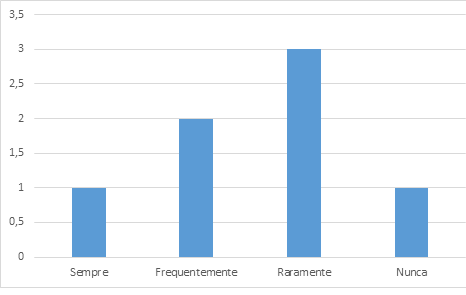
\includegraphics[width=0.85\textwidth]{frequencia em que os alunos utilizam porcentagem.png}
    \label{frequencia em que os alunos utilizam porcentagem}

    {\footnotesize Fonte:  Dados da Pesquisa}
  \end{figure}

  Esse padrão sugere que, embora possuam algum conhecimento básico sobre o tema, muitos alunos têm pouca prática em aplicar porcentagens em situações cotidianas.

  Segundo Souza et al. (\citeyear{souza2022desafios}), essa lacuna entre o conhecimento teórico e a aplicação prática é comum, destacando a importância de estratégias educacionais que conectam conteúdos matemáticos a contextos reais, promovendo uma aprendizagem mais significativa e funcional.

  Em relação à habilidade de calcular aumentos ou reduções percentuais em preços ou valores (Figura \ref{habilidade em calcular aumento ou redução percentuaç}), a maioria dos alunos indicou que possui conhecimento básico, embora ocasionalmente se confunda. Isso demonstra que, embora entendam o conceito, muitos ainda acham dificuldades em aplicar o cálculo com soluções em diferentes contextos.

  Quanto ao nível de confiança dos alunos para realizar cálculos envolvendo porcentagens, figura \ref{nivel de confiança ao fazer calculos}, a maioria das respostas situava-se entre "Baixo" e "Moderado", demonstrando que muitos alunos se sentem inseguros ao aplicar porcentagens, indicando uma necessidade de reforço nessa habilidade para aumentar sua autoconfiança e precisão nos cálculos.
  \\
  \begin{figure}[h!]
    \centering
    \caption{Habilidade em Calcular Um Aumento ou Redução Percentual em um Preço ou Valor
    }
    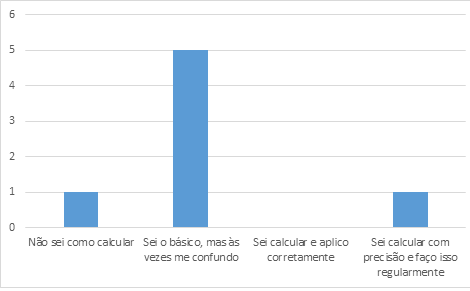
\includegraphics[width=0.85\textwidth]{habilidade de calcular aumento ou redução percentual.png}
    \label{habilidade em calcular aumento ou redução percentuaç}

    {\footnotesize Fonte:  Dados da Pesquisa}
  \end{figure}
  \\
  \\
  \begin{figure}[h!]
    \centering
    \caption{Nível de Confiança dos Alunos ao Fazer Cálculos Envolvendo Porcentagens
    }
    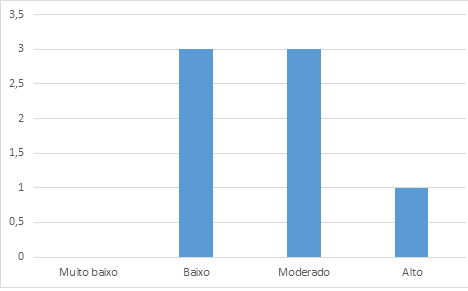
\includegraphics[width=0.85\textwidth]{nivel de confiança ao fazer calculos.png}
    \label{nivel de confiança ao fazer calculos}

    {\footnotesize Fonte:  Dados da Pesquisa}
  \end{figure}

  No que tange à autopercepção dos alunos sobre sua habilidade de calcular porcentagens mentalmente, sem o auxílio de uma calculadora, conforme Figura \ref{habilidade de calcular porcentagem mentalmente}, a maioria avaliou essa competência como "fraca", indicando que muitos alunos enfrentam dificuldades na realização desses cálculos de cabeça e evidenciando a necessidade de práticas adicionais para fortalecer essas habilidades matemáticas básicas.

  Conforme destacado por Parras (\citeyear{Parras2019}):

  \begin{citacao}
    O que chamaremos de design mental vai além do design mental tradicional ou automatizado, incluiremos o design pensado ou fundamentado, que torna possível reconstruir os cálculos por cálculos adequados, bem como cálculo mental literal (\cite{Parras2019},, p. 189).
  \end{citacao}

  Essa observação ressalta a importância de práticas educativas que incentivam o desenvolvimento do projeto mental, passando a capacitar os alunos a realizarem operações básicas sem dependência de ferramentas auxiliares.
  \\
  \begin{figure}[h!]
    \centering
    \caption{Como o aluno avalia sua habilidade de calcular porcentagem mentalmente
    }
    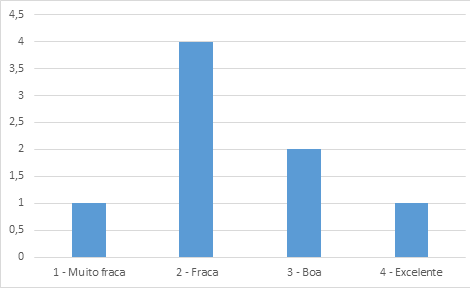
\includegraphics[width=0.85\textwidth]{habilidade de calcular porcentagem mentalmente.png}
    \label{habilidade de calcular porcentagem mentalmente}

    {\footnotesize Fonte: Dados da Pesquisa}
  \end{figure}

  Por fim, ao serem questionados sobre a importância do conhecimento em porcentagem para a gestão financeira pessoal, a maioria dos alunos respondeu que considera esse conhecimento "muito importante", como visto na Figura \ref{sobre acreditar que o conhecimento em porcentagem é essencial}. Essa percepção indica um entendimento generalizado de que porcentagem é fundamental para tomar decisões financeiras acertadas, como avaliar juros, descontos e planejamentos orçamentários.
  \\\begin{figure}[h!]
    \centering
    \caption{Sobre Acreditar Que o Conhecimento em Porcentagem é Essencial Para a Gestão Financeira Pessoal
    }
    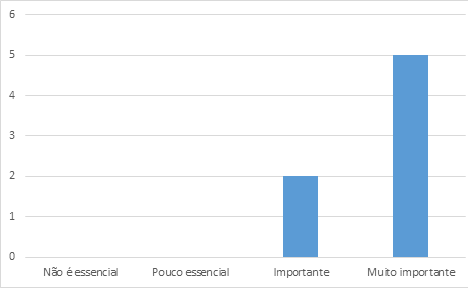
\includegraphics[width=0.85\textwidth]{sobre acreditar que o conhecimento em porcentagem é essencial.png}
    \label{sobre acreditar que o conhecimento em porcentagem é essencial}

    {\footnotesize Fonte:  Dados da Pesquisa}
  \end{figure}
  \\




  \section{Análise do Pré - Teste}

  Em relação ao pré-teste (Apêndice \ref{ApendiceB}), o objetivo foi identificar e analisar o nível de compreensão dos alunos sobre porcentagem antes da intervenção pedagógica. Para isso, a quantidade de acertos e erros em cada questão foi representada em um gráfico (Figura \ref{teste de conhecimentos prévios em porcentagem}).
  \\
  \begin{figure}[h!]
    \centering
    \caption{Teste de Conhecimentos Prévios em Porcentagem
    }
    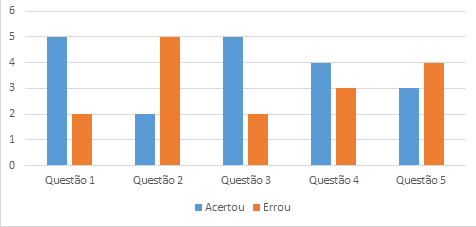
\includegraphics[width=0.85\textwidth]{Teste de conhecimentos prévios em porcentagem.png}
    \label{teste de conhecimentos prévios em porcentagem}

    {\footnotesize Fonte:  Dados da Pesquisa}
  \end{figure}

  Essa estrutura permite uma visão clara e detalhada do desempenho inicial dos estudantes, fornecendo subsídios para entender as principais dificuldades e estabelecer um ponto de partida para o desenvolvimento das atividades propostas na pesquisa.

  Os erros observados no teste de conhecimentos prévios sobre porcentagem revelaram padrões que indicaram dificuldades específicas entre os alunos. Em diversas questões, como nas questões 1, 2, 3 e 5, houve uma recorrente ausência de vírgula na resposta final, evidenciando a dificuldade em lidar com casas decimais (Figura \ref{Ausência de Vírgula na Resposta Final}).

  Essa dificuldade é comum entre estudantes, conforme destacado por Ribeiro (\citeyear{ribeiro2011abordagem}): “O conceito de unidade tem um papel fundamental no estudo dos números e poderá, se não for devidamente explorado, ser uma fonte de dificuldade para os alunos quando trabalham os números racionais (em particular, os decimais)” (\cite{ribeiro2011abordagem},, p. 37).

  Isso ressalta a importância de uma abordagem pedagógica que enfatize a compreensão das unidades e das representações decimais, superando as dificuldades na manipulação de casas decimais.

  \\
  \begin{figure}[h!]
    \centering
    \caption{Ausência de Vírgula na Resposta Final
    }
    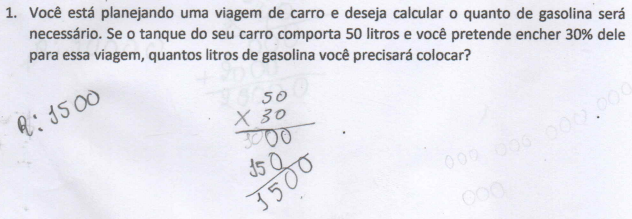
\includegraphics[width=1\textwidth]{Ausência de vírgula na resposta final.png}
    \label{Ausência de Vírgula na Resposta Final}
    {\footnotesize Fonte:  Protocolo de Pesquisa}
  \end{figure}
  \\

  Além disso, nas questões 2 e 4, muitos alunos ficaram confusos com a forma correta da porcentagem, especialmente ao aplicar descontos, deixando o resultado incompleto ou apresentando o valor sem a aplicação do desconto, como pode ser visto na Figura \ref{resultado sem aplicação do desconto}. Essa dificuldade está alinhada com os achados de Souza e Nogueira (\citeyear{souza2020aplicacao}), que apontam:

  \begin{citacao}
    Muitos alunos demonstram dificuldades em compreender a lógica subjacente ao cálculo de porcentagens, especialmente quando aplicados em situações práticas, como descontos ou acréscimos. Esse desafio está frequentemente relacionado à falta de entendimento do conceito de proporcionalidade e à incapacidade de realizar associações entre os cálculos matemáticos e os contextos do cotidiano (\cite{souza2020aplicacao},, p. 23).
  \end{citacao}

  Essa observação reforça a necessidade de estratégias pedagógicas que conectem conteúdos matemáticos a cenários reais, promovendo uma aprendizagem mais significativa.
  \\
  \begin{figure}[h!]
    \centering
    \caption{Resultado Sem Aplicação de Desconto
    }
    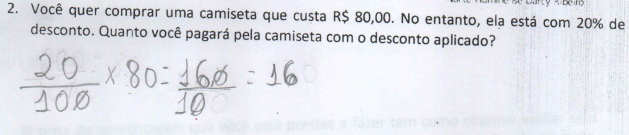
\includegraphics[width=1\textwidth]{Resultado sem aplicação do desconto.png}
    \label{resultado sem aplicação do desconto}
    {\footnotesize Fonte:  Dados da Pesquisa}
  \end{figure}

  Outro erro comum foi o posicionamento indevido da vírgula, particularmente na questão 4, além de dificuldades na interpretação do problema, como observado na questão 5, onde alguns alunos não conseguiram aplicar corretamente as instruções do enunciado (Figura \ref{Interpretação Incorreta do Enunciado}).
  \\
  \begin{figure}[h!]
    \centering
    \caption{Interpretação Incorreta do Enunciado
    }
    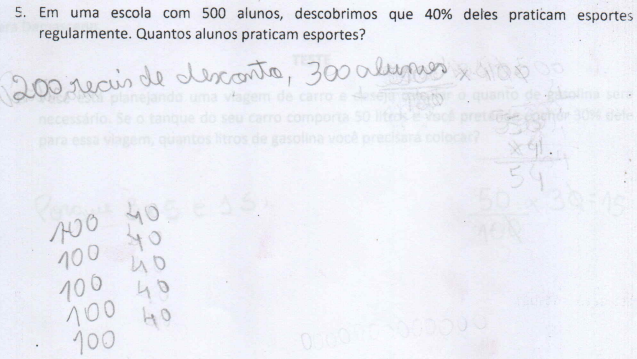
\includegraphics[width=1\textwidth]{interpretação incorreta do enunciado.png}
    \label{Interpretação Incorreta do Enunciado}
    {\footnotesize Fonte:  Dados da Pesquisa}
  \end{figure}
  \\

  Essas dificuldades são frequentemente associadas à falta de compreensão do sistema de numeração decimal e à habilidade de leitura e interpretação de textos matemáticos. Conforme destacado por Lopes (\citeyear{lopes2011leitura}): “As dificuldades apresentadas por muitos alunos para resolver problemas e exercícios matemáticos estão associadas às poucas habilidades que possuem para ler e interpretar os exercícios” (\cite{lopes2011leitura},, p. 14).

  Esse dado indica a importância de desenvolver nas aulas competências de leitura e interpretação de enunciados matemáticos, bem como uma compreensão sólida do sistema de numeração decimal, para que se possa superar essas dificuldades.

  Os erros identificados no teste de conhecimentos prévios sobre porcentagem refletiram áreas de fragilidade no domínio de conceitos fundamentais, como o uso de casas decimais e a aplicação correta de descontos. A atenção a essas dificuldades específicas permitiu que o processo de ensino fosse direcionado, para uma aprendizagem mais significativa e precisa, promovendo o desenvolvimento das competências essenciais para o cálculo e interpretação de porcentagens.




  \section{Análise da Sequência Didática}

  Para realizar a sequência didática proposta foram necessários 3 encontros, com duração de 3 horas, utilizando a metodologia de Rotação por Estações e ABP para diversificar o aprendizado e promover uma experiência dinâmica.

  Na utilização da metodologia Rotação por Estações, a sala de aula foi estruturada em três estações temáticas, cada uma com foco em diferentes habilidades, e os alunos foram distribuídos em três grupos de quatro membros.

  Antes do início das atividades, foi realizada uma breve apresentação sobre o funcionamento da metodologia, com explicação na lousa sobre o propósito de cada estação e os objetivos gerais do percurso de aprendizagem. Esta introdução ofereceu aos alunos autonomia para escolherem a sequência de estações que desejavam seguir, promovendo a integração colaborativa e a construção de uma experiência de aprendizagem personalizada.

  Segundo Sefton e Galini (\citeyear{sefton2020metodologias}), a autonomia é um elemento-chave nas metodologias ativas, pois permite que os estudantes assumam papéis protagonistas em seu aprendizado, ao mesmo tempo em que desenvolvem competências como a colaboração e a resolução de problemas.

  Essa abordagem está alinhada às competências gerais da Educação Básica, em conformidade com as diretrizes da BNCC, que destacam a importância de "agir pessoal e coletivamente autonomia, responsabilidade, flexibilidade, resiliência e determinação, tomando com base em princípios éticos, democráticos, inclusivos, sustentáveis e solidários” (\cite{Educacao.2018},, p. 12). Tais competências foram incentivadas ao longo da atividade, estimulando nos alunos a capacidade de adaptação e o fortalecimento de habilidades socioemocionais essenciais.

  Cada equipe recebeu um conjunto de materiais específicos para organizar seu trabalho, incluindo uma página destinada a registros e anotações, uma folha de instruções elaborada sobre as tarefas a serem realizadas em cada estação e um caderno de apoio para a execução e pesquisa das atividades propostas. Esses documentos estão disponíveis no Apêndice C desta dissertação e serviram como guias para manter o foco e facilitar o aprendizado independente em cada estação.

  Cada grupo participava em cada estação por um período de uma hora, garantindo que todos pudessem participar de todas as atividades planejadas e experimentar diversas abordagens de aprendizagem. Essa estrutura permitiu que os alunos vivenciassem diferentes perspectivas e se envolvessem ativamente em sua formação.

  De acordo com Sefton e Galini (\citeyear{sefton2020metodologias}), o uso de metodologias ativas, como o Rotação por Estações, proporciona aos estudantes a oportunidade de interagir com conteúdos diversos de maneira prática e dinâmica, promovendo uma aprendizagem mais significativa e contextualizada.




  \subsection{Análise da Estação de Otimização do Orçamento Familiar}

  Nesta estação, os alunos trabalharam com uma planilha no Excel que simulava um orçamento doméstico fictício (Figura \ref{orçamento doméstico fictício}). A proposta envolve calcular a porcentagem correspondente de cada despesa em relação ao total do orçamento (Figura \ref{estação de otimização do orçamento familiar}), promovendo uma compreensão prática do conceito de percentagem.

  Em seguida, foram orientados a usar esses valores percentuais para construir um gráfico de pizza. Essa abordagem está alinhada com as práticas recomendadas pelo Banco Central do Banco Central do Brasil:

  \begin{citacao}
    Reconhecer o orçamento como ferramenta para a compreensão dos próprios hábitos de consumo. Aplicar os conceitos de receitas e despesas na elaboração do orçamento, para torná-lo superavitário. Utilizar o orçamento para o planejamento financeiro pessoal e familiar (\cite{bancocentral2013_educacao_financeira},, pág. 9).
  \end{citacao}

  Essa metodologia visa fortalecer as habilidades matemáticas básicas dos alunos, incentivando a aplicação prática dos conceitos aprendidos.
  \\
  \begin{figure}[h!]
    \centering
    \caption{Estação de Otimização do Orçamento Familiar
    }
    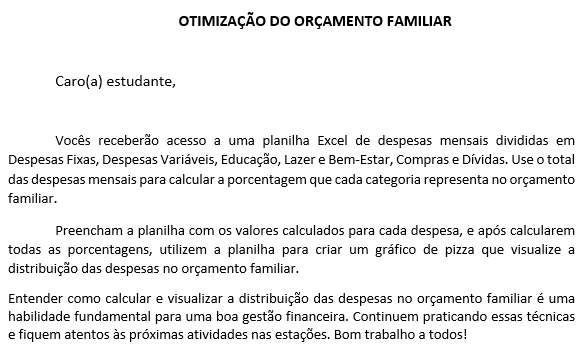
\includegraphics[width=1\textwidth]{Estação de Otimização do Orçamento Familiar.png}
    \label{estação de otimização do orçamento familiar}
    {\footnotesize Fonte:  Dados da Pesquisa}
  \end{figure}
  \\
  \\
  \begin{figure}[h!]
    \centering
    \caption{Orçamento Doméstico fictício
    }
    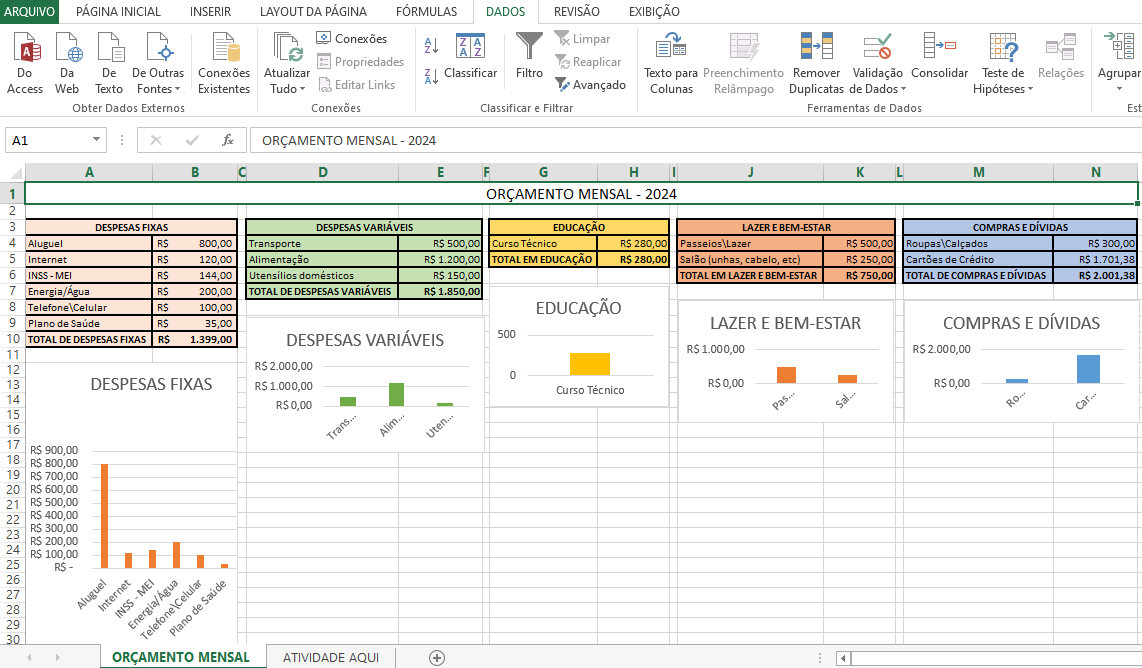
\includegraphics[width=1\textwidth]{orçamento doméstico fictício.png}
    \label{orçamento doméstico fictício}
    {\footnotesize Fonte:  Dados da Pesquisa}
  \end{figure}
  \\

  Durante a atividade, alguns alunos enfrentaram dificuldades para realizar o cálculo de porcentagens a partir de valores específicos, necessitando de suporte adicional e, em alguns casos, consultando recursos online para compreender melhor o processo. Após superarem essa etapa e adquirirem o entendimento necessário, obtiveram os cálculos de forma precisa, conforme demonstrado na Figura \ref{cálculos dos alunos}.
  \\
  \begin{figure}[h!]
    \centering
    \caption{Cálculos dos Alunos
    }
    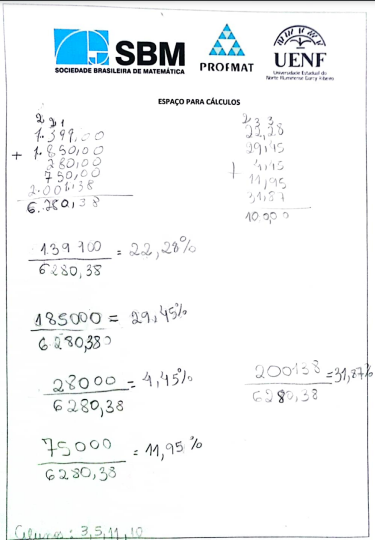
\includegraphics[width=0.85\textwidth]{Cáculos dos alunos.png}
    \label{cálculos dos alunos}

    {\footnotesize Fonte:  Dados da Pesquisa}
  \end{figure}
  \\

  Essa situação reflete os desafios descritos por Campos e Silva (\citeyear{campos2021ensino}) que afirma:
  \begin{citacao}
    A dificuldade de muitos alunos em lidar com porcentagens e cálculos relacionados advém, em grande parte, da falta de conexão entre o conteúdo ensinado e as aplicações práticas do dia a dia. Quando inseridos em contextos reais ou apoiados por ferramentas tecnológicas, os estudantes demonstram maior engajamento e conseguem compreender melhor os conceitos matemáticos envolvidos (\cite{campos2021ensino},, p. 12).
  \end{citacao}

  Essa constatação enfatiza a importância de conectar conteúdos matemáticos a situações cotidianas, favorecendo uma aprendizagem mais prática.

  A criação do gráfico de pizza representou um desafio para os alunos, que tiveram sua primeira experiência com o uso do Excel e a manipulação de dados em um computador (Figura \ref{alunos na atividade de orçamento familiar}).
  \\
  \begin{figure}[h!]
    \centering
    \caption{Alunos Realizando as Atividades na Estação de Otimização do Orçamento Familiar
    }
    \includegraphics[width=1\textwidth]{alunos na estação de orçamento familiar.jpg}
    \label{alunos na atividade de orçamento familiar}

    {\footnotesize Fonte:  Dados da Pesquisa}
  \end{figure}

  A professora esteve presente para orientar cada grupo, guiando-os na inserção dos dados, na configuração do gráfico e no entendimento visual das proporções representadas. Conforme descrito por Prado e Silva (\citeyear{prado2019tecnologias}):
  \begin{citacao}
    A utilização de ferramentas tecnológicas no ensino de matemática permite não apenas o aprendizado de conceitos matemáticos, mas também o desenvolvimento de competências digitais. Quando os estudantes aplicam tecnologias em atividades práticas, como a criação de gráficos, eles constroem uma conexão mais significativa com os conteúdos e regulam sua aplicabilidade no cotidiano (\cite{prado2019tecnologias},, p. 47).
  \end{citacao}

  Essa abordagem prática reforça a importância de integrar tecnologias ao ensino para promover uma aprendizagem contextualizada.Esse apoio foi essencial para que os alunos concluíssem a tarefa, promovendo uma aprendizagem colaborativa e prática, como retratado na figura \ref{atividade resolvida pelos alunos}.
  \\
  \begin{figure}[h!]
    \centering
    \caption{Atividade Resolvida Pelos Alunos
    }
    \includegraphics[width=1\textwidth]{atividade resolvida pelos alunos.png}
    \label{atividade resolvida pelos alunos}

    {\footnotesize Fonte:  Dados da Pesquisa}
  \end{figure}

  A atividade proporcionou aos alunos uma experiência prática e significativa no uso de planilhas eletrônicas para cálculos percentuais e na construção de gráficos, habilidades fundamentais tanto para a compreensão de matemática aplicada quanto para o desenvolvimento de competências digitais. Apesar dos desafios iniciais, especialmente para aqueles sem familiaridade com o uso de computadores, o suporte da professora e a aprendizagem colaborativa entre os colegas foram essenciais para que superassem essas dificuldades.

  De acordo com Moran (\citeyear{moran2015metodologias}), atividades que integram e trabalho colaborativo não apenas reforçam a compreensão dos conteúdos, mas também promovem o desenvolvimento de competências essenciais para a vida acadêmica e profissional, como autonomia, criatividade e capacidade de resolver problemas cotidianos.

  Assim, a atividade se mostrou eficiente ao promover a autonomia, a capacidade de resolução de problemas e o trabalho em equipe, elementos indispensáveis para o desenvolvimento acadêmico e profissional dos alunos.





  \subsection{Análise da Estação de Controle Orçamentário}

  Nesta estação, os alunos foram desafiados a trabalhar com um orçamento familiar fictício, uma atividade que alia matemática e desenvolvimento de habilidades práticas. O probela começou com a análise de um orçamento-base, no qual eles deveriam ajustar proporcionalmente os valores destinados a diferentes categorias, como alimentação, transporte, lazer e educação, considerando um aumento pré-determinado na renda familiar. Para promover um aprendizado significativo, foram incentivados a aplicar suas escolhas, refletindo sobre as prioridades de cada família.

  Conforme destacado por Kappaun (\citeyear{kappaun2017orcamento}):
  \begin{citacao}
    O trabalho com orçamento familiar em sala de aula permite aos alunos compreender a importância do planejamento financeiro, bem como desenvolver habilidades matemáticas aplicadas ao cotidiano. Ao simular situações reais, os estudantes são levados a refletir sobre a distribuição de recursos e a tomada de decisões conscientes  (\cite{kappaun2017orcamento},, p. 15).
  \end{citacao}

  Isso fortalece compreensão dos alunos sobre a gestão financeira e a aplicação de conceitos matemáticos em contextos reais.
  Após essa etapa, os alunos receberam uma segunda tarefa: reduzir o valor total ajustado em 10\%, com o objetivo de criar uma reserva financeira para situações de emergência. Essa redução promoveu o desenvolvimento de cálculos precisos e um olhar estratégico para redistribuir os valores sem comprometer necessidades básicas.

  A proposta teve como objetivo não apenas desenvolver competências matemáticas, como proporção e porcentagem, mas também estimular a educação financeira e a tomada de decisões conscientes no gerenciamento de recursos, conforme ilustrado nas Figuras \ref{estação de controle orçamentário} e \ref{orçamento doméstico fictício (2)}.

  Essa abordagem está alinhada com as diretrizes do Banco Central do Brasil, que enfatiza:
  \begin{citacao}
    A educação financeira visa capacitar o cidadão a tomar decisões conscientes e bem informadas sobre a gestão de seus recursos, promovendo o planejamento financeiro e a formação de poupança, de modo a prevenir o endividamento excessivo e contribuir para a estabilidade do sistema financeiro (\cite{bancocentral2013_educacao_financeira},, p. 5).
  \end{citacao}
  \\
  \begin{figure}[h!]
    \centering
    \caption{Estação de Controle Orçamentário
    }
    \includegraphics[width=1\textwidth]{estação de controle orçamentário.png}
    \label{estação de controle orçamentário}

    {\footnotesize Fonte:  Dados da Pesquisa}
  \end{figure}
  \\
  \\
  \begin{figure}[h!]
    \centering
    \caption{Orçamento Doméstico Fictício
    }
    \includegraphics[width=0.4\textwidth]{orçamento doméstico fictício (2).png}
    \label{orçamento doméstico fictício (2)}

    {\footnotesize Fonte: Dados da Pesquisa}
  \end{figure}
  \\

  Essa atividade buscou integrar conceitos matemáticos e financeiros, preparando os alunos para uma gestão responsável de seus recursos no futuro.

  Nesta atividade foi permitido o uso da calculadora devido à grande quantidade de cálculos envolvidos, considerando o tempo limitado de uma hora para a conclusão das tarefas. Essa decisão visava agilizar o processo, permitindo que os alunos se concentrassem mais no raciocínio lógico e na compreensão do problema do que na execução dos cálculos manuais.

  Além disso, a atividade ressaltou a importância de saber usar uma calculadora de forma assertiva, garantindo que a ferramenta fosse utilizada como um recurso para aumentar a precisão e a eficiência, e não como um substituto para o entendimento matemático. Ao aprenderem a utilizá-la corretamente, os alunos desenvolvem uma habilidade prática que será útil em diversos contextos do dia-a-dia.

  Conforme destacado por Sobreira et al. (\citeyear{sobreira2021uso}):  "O uso didático da calculadora propicia melhores condições de aprendizagem no âmbito da Matemática, que por sua vez busca formar pessoas reflexivas diante de fatos ao seu redor, bem como capazes de tomar decisões" (\cite{sobreira2021uso},, p. 19).

  Essa análise destaca a necessidade de integrar ferramentas tecnológicas ao ensino, promovendo uma compreensão mais profunda dos conceitos matemáticos e preparando os alunos para desafios do dia-a-dia.

  Apesar da ferramenta, alguns equívocos foram cometidos, principalmente na aplicação das operações de porcentagem. Observando as dificuldades, a professora interveio para orientar os alunos a adotarem uma abordagem mais estruturada. Foi sugerido que dividissem os cálculos em etapas, começando pelo cálculo da porcentagem requerida e, em seguida, adicionando ou subtraindo o resultado do valor inicial.

  Essa estratégia está em conformidade com os princípios defendidos por Ribeiro (\citeyear{ribeiro2019ensinar}), que destaca a importância de ensinar métodos sistemáticos e passo a passo para resolver problemas matemáticos, promovendo uma compreensão mais profunda dos conceitos e uma redução significativa dos erros comuns. Ao aplicar essa abordagem, os alunos poderão revisar e corrigir seus erros, aprimorando sua precisão e compreensão.

  Esse método não apenas facilitou a resolução das atividades, como também contribuiu para que os alunos internalizassem uma forma prática e eficaz de lidar com cálculos percentuais em situações do cotidiano. O sucesso dessa abordagem ficou evidente no resultado final, representado nas Figuras \ref{calculos dos alunos (2)}\ \ref{atividade dos alunos respondida}, \ref{cálculos dos alunos (3)} e \ref{atividade dos alunos respondida (2)}, que ilustram o progresso dos alunos ao reorganizarem o orçamento financeiro com mais segurança e eficiência.

  De acordo com Carvalho (\citeyear{carvalho2018educacao}), metodologias que conectam a aprendizagem matemática a situações reais do dia a dia favorecem a internalização dos conceitos, aumentando a segurança dos alunos na aplicação prática e promovendo o desenvolvimento de habilidades transferíveis para diferentes contextos da vida.
  \\
  \\
  \begin{figure}[h!]
    \centering
    \caption{Cáculos dos Alunos
    }
    \includegraphics[width=1\textwidth]{cálculos dos alunos (2).png}
    \label{calculos dos alunos (2)}

    {\footnotesize Fonte:  Dados da Pesquisa}
  \end{figure}
  \\

  \\
  \begin{figure}[h!]
    \centering
    \caption{Atividade Resolvida Pelos Alunos
    }
    \includegraphics[width=0.45\textwidth]{Atividade resposndida (2).png}
    \label{atividade dos alunos respondida}

    {\footnotesize Fonte:  Dados da Pesquisa}
  \end{figure}
  \\

  \\
  \begin{figure}[h!]
    \centering
    \caption{Cálculos dos Alunos
    }
    \includegraphics[width=0.65\textwidth]{cálculos(3).png}
    \label{cálculos dos alunos (3)}

    {\footnotesize Fonte:  Dados da Pesquisa}
  \end{figure}
  \\

  \\
  \begin{figure}[h!]
    \centering
    \caption{Atividade Resolvida pelos Alunos
    }
    \includegraphics[width=0.5\textwidth]{atividade dos alunos respondida (2).png}
    \label{atividade dos alunos respondida (2)}

    {\footnotesize Fonte:  Dados da Pesquisa}
  \end{figure}
  \\

  Os alunos obtiveram grande satisfação ao conseguirem concluir com sucesso a atividade proposta. Era evidente, pelo brilho em seus olhos e pelos sorrisos no rosto, o orgulho e a alegria de superar os desafios apresentados. A sensação de conquista foi reforçada à medida que adquirimos sua capacidade de aplicar conhecimentos matemáticos em uma situação prática e desafiadora.

  Segundo Santos (\citeyear{santos2020matematica}), atividades que promovem a resolução de problemas em contextos práticos não apenas favorecem o aprendizado de conceitos matemáticos, mas também são fundamentais para o desenvolvimento de autoestima e confiança dos alunos, elementos fundamentais para seu progresso acadêmico e pessoal.

  Essa experiência não apenas reforçou a confiança deles em suas habilidades, mas também gerou um sentimento de realização pessoal, mostrando que, com esforço e orientação adequada, eram capazes de resolver problemas reais de forma eficaz.

  Na imagem adiante (Figura \ref{alunos resolvendo as atividades}), é possível observar os alunos concentrados, discutindo em pequenos grupos e utilizando uma calculadora como ferramenta de apoio. A postura atenta e a clara em cada interação evidenciam o envolvimento e a dedicação deles durante toda a atividade.

  \begin{figure}[h!]
    \centering
    \caption{Alunos Resolvendo as Atividades
    }
    \includegraphics[width=1\textwidth]{alunos resolvendo as atividades (2).jpg}
    \label{alunos resolvendo as atividades}

    {\footnotesize Fonte:  Protocolo de Pesquisa}
  \end{figure}

  Conforme apontado por Santos (\citeyear{santos2020matematica}):
  \begin{citacao}
    Ao trabalhar com problemas que envolvem contextos reais, os alunos passam a enxergar a matemática como uma ferramenta útil e aplicável, o que aumenta significativamente o engajamento e a motivação. Esse tipo de atividade estimula a interação em grupo, permitindo que os estudantes aprendam uns com os outros, enquanto desenvolvem habilidades de comunicação, cooperação e pensamento crítico (\cite{santos2020matematica},, p. 58).
  \end{citacao}

  Isso demonstra como atividades contextualizadas podem transformar o aprendizado em uma experiência enriquecedora.

  A proposta de atividade aos alunos não é apenas uma oportunidade de aplicar conceitos matemáticos em um contexto prático, mas também um momento de crescimento pessoal e acadêmico. O uso da calculadora, aliada à orientação pedagógica, revelou-se uma estratégia eficiente para lidar com os desafios apresentados, destacando a importância de compreender e dominar as ferramentas tecnológicas disponíveis.

  A satisfação expressa pelos alunos ao final da tarefa reafirmou o valor de propor atividades significativas, que estimulam o aprendizado colaborativo e promovem o desenvolvimento de habilidades essenciais para a vida. Conforme descrito por Ribeiro (\citeyear{ribeiro2019ensinar}):

  \begin{citacao}
    Ao integrar ferramentas tecnológicas e atividades práticas ao ensino de matemática, os alunos desenvolvem não apenas competências acadêmicas, mas também habilidades pessoais, como resiliência e autoconfiança. Esses elementos são fundamentais para que os estudantes enfrentem os desafios da vida acadêmica e profissional com mais segurança e capacidade de resolver problemas (\cite{ribeiro2019ensinar},, p. 67).
  \end{citacao}

  Essa experiência, além de fortalecer os conhecimentos matemáticos, contribuiu para aumentar a autoconfiança dos estudantes, preparando-os para enfrentar os desafios da vida cotidiana com mais segurança e autonomia.





  \subsection{Análise da Estação de Jogos Educativos}

  Na \textbf{Estação de Jogos Educativos} , os alunos participaram de uma atividade interativa voltada para a educação financeira, envolvendo dois jogos que incentivaram a aprendizagem de forma prática e divertida. No primeiro jogo, acessado através da plataforma \textbf{Wordwall.net} e intitulado \textit{Atividade sobre Educação Financeira - Game Show de TV }, os alunos responderam a um quiz com perguntas relacionadas a conceitos como orçamento, consumo consciente e planejamento financeiro.

  A experiência foi detalhada no Capítulo 4, item \ref{subsec:encontro2} - Encontro 2, e teve como objetivo consolidar o aprendizado de forma colaborativa. Durante a atividade, os alunos se revezaram, interagiram entre si e discutiram estratégias para responder corretamente às perguntas. A dinâmica competitiva típica de um game show tornou o momento ainda mais envolvente, estimulando não apenas o aprendizado, mas também o trabalho em equipe. Como ressaltam Sefton e Galini (\citeyear{sefton2020metodologias}):
  \begin{citacao}
    O uso de dinâmicas interativas e colaborativas, como jogos educacionais, tem o potencial de transformar o aprendizado em uma experiência significativa. Ao envolver os estudantes em atividades que envolvem competição saudável e cooperação, eles não apenas aprendem os conteúdos, mas também desenvolvem habilidades interpessoais, como comunicação, trabalho em equipe e resolução de problemas (\cite{sefton2020metodologias},, p. 92).
  \end{citacao}


  Isso mostra a eficácia de metodologias que aliam interação social e aprendizado, proporcionando um ambiente educativo mais dinâmico e participativo.

  Nas imagem adiante é possível observar os alunos em plena interação com o jogo. Na primeira imagem (Figura \ref{alunos concentrados nas perguntas na tela}), eles aparecem concentrados nas perguntas exibidas na tela, demonstrando comprometimento em encontrar a resposta correta.
  \\
  \begin{figure}[h!]
    \centering
    \caption{Concentração ao Ver as Perguntas na Tela
    }
    \includegraphics[width=0.4\textwidth]{Alunos concentrados nas perguntas na tela.png}
    \label{alunos concentrados nas perguntas na tela}

    {\footnotesize Fonte:  Dados da Pesquisa}
  \end{figure}

  Na segunda imagem (Figura \ref{Alunos Comemorando os Pontos Conquistados}), vemos um grupo comemorando os pontos conquistados, o que reflete a entusiasmo e a satisfação que a atividade proporcionou. Esses registros destacam a importância de aliar tecnologia e diversão para promover uma aprendizagem significativa e engajadora.
  \\
  \begin{figure}[h!]
    \centering
    \caption{Alunos Comemorando os Pontos Conquistados
    }
    \includegraphics[width=1\textwidth]{alunos comemorando os pontos conquistados.jpg}
    \label{Alunos Comemorando os Pontos Conquistados}

    {\footnotesize Fonte:  Dados da Pesquisa}
  \end{figure}

  O segundo jogo, descrito no Capítulo 4, item \ref{subsec:encontro2} - Encontro 2 dessa pesquisa, é intitulado \textit{Vamos Relembrar Alguns Conceitos do Semestre de Educação Financeira - Perseguição em Labirinto}, disponível na plataforma Wordwall.net. Nesta atividade, os alunos conduziram um astronauta por um labirinto em busca das respostas corretas para perguntas relacionadas à educação financeira, revisando conceitos estratégicos ao longo das atividades, como orçamento, poupança, consumo consciente e planejamento financeiro.

  A dinâmica do jogo requer que os participantes combinem raciocínio lógico, foco e agilidade para escolher rapidamente o caminho correto. Além disso, o cenário criativo de exploração espacial, com o astronauta navegando pelos desafios, tornou-se uma experiência ainda mais envolvente, incentivando o engajamento e o interesse dos alunos. O jogo, ao mesmo tempo que revisava conteúdos essenciais, proporcionava momentos de diversão e trabalho em equipe, tornando a aprendizagem significativa e prazerosa.

  Nas imagens adiante, Figuras \ref{Grupo Discutindo Melhores Estratégias Para o Jogo} e \ref{Aluno interagindo com o jogo}, é possível observar os alunos imersos na atividade. Na primeira imagem, eles aparecem discutindo em grupo a escolha do melhor caminho no labirinto, demonstrando colaboração e estratégia. Na segunda imagem, um aluno interage diretamente com o jogo, evidenciando a concentração e a motivação que a atividade gerou.
  \\
  \begin{figure}[h!]
    \centering
    \caption{Grupo Discutindo Melhores Estratégias Para o Jogo
    }
    \includegraphics[width=1\textwidth]{grupo discutindo estratégias.jpg}
    \label{Grupo Discutindo Melhores Estratégias Para o Jogo}

    {\footnotesize Fonte:  Dados da Pesquisa}
  \end{figure}

  \\
  \begin{figure}[h!]
    \centering
    \caption{Aluno Interagindo com o jogo
    }
    \includegraphics[width=1\textwidth]{aluno jogando.jpg}
    \label{Aluno interagindo com o jogo}

    {\footnotesize Fonte:  Dados da Pesquisa}
  \end{figure}

  Esses registros mostram como o uso de ferramentas lúdicas pode transformar o aprendizado em uma experiência enriquecedora e estimulante. Conforme destacado por Moran (\citeyear{moran2015metodologias}):
  \begin{citacao}
    O aprendizado lúdico proporciona aos estudantes um ambiente de exploração criativa, onde o erro é visto como parte do processo e a colaboração é incentivada. Atividades lúdicas ajudam a construir um aprendizado mais significativo e engajador, conectando emoções e raciocínio lógico em uma experiência única ( \cite{moran2015metodologias},, p. 47).
  \end{citacao}

  Embora esse jogo apresente uma menor complexidade e tenha sido idealizado, no primeiro momento, para incluir dois alunos com necessidades educacionais especiais, sua proposta lúdica e interativa acabou conquistando todos os estudantes. A dinâmica envolvente e o desafio de dirigir o astronauta pelo labirinto de forma ágil e assertiva despertaram a paixão da turma, tornando uma atividade inclusiva e prazerosa para todos. Conforme apontado por Vygotsky (\citeyear{vigotsky1998}):
  \begin{citacao}
    O brincar contém em si todas as tendências do desenvolvimento em forma condensada, sendo em si mesmo uma fonte poderosa para o crescimento cultural da criança. Ao brincar, os indivíduos não apenas reproduzem experiências, mas também as transformam em novas formas de organização mental e social, estimulando a colaboração e o aprendizado (\citeyear{vigotsky1998},, p. 73).
  \end{citacao}

  A emoção gerada pela experiência foi tamanha que muitos alunos expressaram o desejo de continuar jogando por mais tempo, evidenciando o quanto estavam imersos na atividade. Essa recepção calorosa reforça o valor de jogos educativos bem planejados, capazes de fornecer diferentes níveis de habilidade e proporcionar um ambiente de aprendizagem acolhedor e estimulante. A adaptação inicial para atender alunos com necessidades especiais acabou se revelando um acerto pedagógico, promovendo integração, participação coletiva e diversão.

  A experiência com os jogos educativos demonstrou o potencial das ferramentas lúdicas para enriquecer o aprendizado, promovendo não apenas o conhecimento dos conceitos de educação financeira, mas também a inclusão e o engajamento de todos os alunos. Ao combinar atividades de diferentes níveis de complexidade e contextos interativos, a proposta atende às necessidades individuais dos estudantes, incentivando a colaboração, a criatividade e a excitação pelo aprendizado.

  O sucesso da estação, evidenciado pela diversão e pela participação ativa dos alunos, reforça a importância de integrar metodologias ativas ao planejamento pedagógico. Esses momentos de aprendizado descontraído não apenas consolidam os conteúdos trabalhados em sala, mas também criam memórias positivas que estimulam os estudantes a se envolverem ainda mais no processo educativo. A combinação de tecnologia, inclusão e diversão mostrou uma estratégia eficaz para tornar o aprendizado mais significativo e acessível a todos.




  \subsection{Análise do Problema 1}

  O Problema 1 foi apresentado aos alunos como parte da implementação da ABP. Para garantir que todos compreendessem a atividade, os passos necessários para a resolução foram detalhadamente expostos no quadro, permitindo que os estudantes seguissem uma estrutura organizada e clara durante o processo.

  Segundo Moran (\citeyear{moran2015metodologias}), uma apresentação bem estruturada das etapas de uma atividade é fundamental em metodologias ativas, como a ABP, pois fornece aos alunos um caminho claro para abordar os problemas, ao mesmo tempo em que estimula a autonomia e o pensamento crítico ao longo do processo.

  A partir do primeiro passo, \textbf{Esclarecimentos de Termos e Conceitos}, os alunos iniciaram o trabalho dedicando-se a compreender plenamente o enunciado do problema e a identificar os conceitos fundamentais envolvidos. Essa etapa inicial foi essencial para alinhar o entendimento de todos e estabelecer uma boa base para as próximas fases da atividade. Durante esse processo, surgiram dúvidas em relação aos termos “orçamento”, “renda”, “despesa” e “reserva de emergência”, que eram essenciais para a resolução do problema.

  De acordo com Sefton e Galini (\citeyear{sefton2020metodologias}), a etapa de esclarecimento de conceitos é uma das mais importantes na Aprendizagem Baseada em Problemas, pois permite que os alunos compreendam o contexto do problema e estabeleçam uma linguagem comum, garantindo que as fases seguintes sejam realizadas de forma mais eficiente e colaborativa.

  Para esclarecer essas dúvidas, os alunos utilizaram notebooks disponibilizados pela pesquisadora, acessando a internet para pesquisar e entender o significado de cada termo. Essa iniciativa propôs uma experiência prática de busca por informações e aprendizado independente, promovendo o desenvolvimento de habilidades como pesquisa e análise crítica.

  Após sanar as dúvidas, os alunos registraram os conceitos de forma organizada em uma folha de soluções previamente entregue pela pesquisadora (Figuras \ref{Passo 1} e \ref{Passo 1 - continuação}), garantindo que todos tivessem acesso a um referencial comum para dar continuidade à atividade. Esse processo inicial contribuiu para um aprendizado mais colaborativo, permitindo que os alunos avançassem com maior segurança nas etapas seguintes.

  Segundo Moran (\citeyear{moran2015metodologias}), o registro organizado de conceitos e informações durante atividades pedagógicas não apenas favorece o aprendizado individual, mas também promove a colaboração, ao fornecer uma base comum que facilita o compartilhamento de ideias e a construção coletiva do conhecimento.
  \\
  \\
  \\
  \\
  \begin{figure}[h!]
    \centering
    \caption{Passo 1: Esclarecimento de Termos e Conceitos
    }
    \includegraphics[width=0.65\textwidth]{Passo 1.png}
    \label{Passo 1}

    {\footnotesize Fonte:  Dados da Pesquisa}
  \end{figure}
  \\

  \\
  \begin{figure}[h!]
    \centering
    \caption{Passo 1: Esclarecimento de Termos e Conceitos
    }
    \includegraphics[width=0.65\textwidth]{Passo 1 continuação.png}
    \label{Passo 1 - continuação}

    {\footnotesize Fonte:  Dados da Pesquisa}
  \end{figure}
  \\

  Ao trabalhar coletivamente e compartilhar diferentes interpretações, os estudantes começaram a construir uma compreensão mais profunda do problema, criando um ambiente de aprendizagem que favorece o desenvolvimento de habilidades como análise crítica e organização de ideias. Esse início estruturado proporcionou condições propícias para que o grupo avançasse de forma autônoma na busca por soluções práticas e fundamentadas.

  De acordo com Sefton e Galini (\citeyear{sefton2020metodologias}), o trabalho colaborativo em metodologias como a ABP promove o engajamento dos alunos na construção coletiva do conhecimento, ao permitir que diferentes perspectivas sejam integradas, fortalecendo o raciocínio crítico e a capacidade de resolver problemas de maneira fundamentada e criativa.

  Na segunda etapa, \textbf{Definição do Problema}, os alunos concentraram seus esforços em identificar e detalhar o problema central apresentado: como uma família pode organizar suas finanças para realizar o sonho de comprar um carro, considerando suas fontes de renda, despesas e a importância de manter uma reserva de emergência. Essa etapa ocorreu com os estudantes se aprofundando na análise da situação da família, buscando compreender seus objetivos, limitações e desafios financeiros.

  Segundo Moran (\citeyear{moran2015metodologias}), a etapa de definição do problema em metodologias ativas, como a ABP, é fundamental para contextualizar a aprendizagem, pois permite que os estudantes explorem o problema em sua totalidade, identificando elementos-chave e estabelecendo uma compreensão mais clara dos desafios a serem enfrentados.

  Durante o processo, os alunos discutiram de forma colaborativa os elementos mais importantes para a definição do problema. Aspectos como o sonho de adquirir o carro, a gestão do orçamento familiar, a possibilidade de vender a moto como parte do planejamento e os fatores externos que influenciaram a decisão, como os juros do financiamento e a necessidade de economia, foram extremamente debatidos.

  Esse exercício de reflexão e troca de ideias permitiu que os estudantes formulassem uma visão clara e detalhada do problema, considerando tanto as metas quanto as dificuldades da família. De acordo com Sefton e Galini (\citeyear{sefton2020metodologias}), a reflexão colaborativa é um elemento central na Aprendizagem Baseada em Problemas, pois promove a construção de um entendimento coletivo mais aprofundado, ao integrar diferentes perspectivas e estimular os alunos a analisar as complexidades do problema de forma crítica e detalhada.

  Ao final dessa etapa, os alunos registraram os pontos principais levantados durante a discussão (Figura \ref{Passo 2}), estruturando a definição do problema de forma lógica e bem fundamentada. A experiência reforça habilidades como análise crítica, trabalho em equipe e comunicação, essenciais para a resolução de problemas complexos.

  Segundo Moran (\citeyear{moran2015metodologias}), a documentação e a organização das ideias em metodologias ativas, como a ABP, são fundamentais para consolidar o aprendizado, além de cultivar a colaboração e a troca de perspectivas, habilidades indispensáveis para lidar com desafios acadêmicos e profissionais.
  \\
  \begin{figure}[h!]
    \centering
    \caption{Passo 2: Definição do Problema
    }
    \includegraphics[width=0.65\textwidth]{Passo 2.png}
    \label{Passo 2}

    {\footnotesize Fonte:  Dados da Pesquisa}
  \end{figure}

  No terceiro passo, \textbf{Análise do Problema}, os alunos realizaram uma análise detalhada do cenário apresentado, identificando dados concretos relacionados às finanças da família. Esse processo incluiu o levantamento de informações fundamentais, como as fontes de renda de Dona Maria e Seu João, o valor estimado da motocicleta e os diferentes tipos de despesas familiares. A partir desses dados, os alunos calcularam o saldo mensal disponível, determinando a diferença entre a renda total e os gastos regulares. Como destacado por Sefton e Galini (\citeyear{sefton2020metodologias}):
  \begin{citacao}
    A etapa de análise do problema em metodologias como a ABP é essencial para que os estudantes desenvolvam uma compreensão detalhada do contexto apresentado. Nesse momento, os alunos são desafiados a identificar, organizar e interpretar dados relevantes, conectando-os ao problema central. Essa prática não apenas fortalece habilidades matemáticas e analíticas, mas também promove o pensamento crítico e a capacidade de tomar decisões fundamentadas (\cite{sefton2020metodologias},, p. 88).
  \end{citacao}

  Esse exercício reforçou a importância de habilidades analíticas no contexto educacional, preparando as aulas para situações práticas e perguntas.

  Este passo foi documentado pelo membro mais velho do grupo, que fez questão de registrar sua participação no processo. Por esse motivo, a escrita apresenta traços um pouco trêmulos, figura \ref{Passo 3}, mas reflete o esforço e o engajamento dos participantes em contribuir com a atividade, reforçando o aspecto colaborativo e inclusivo da metodologia.

  \\
  \begin{figure}[h!]
    \centering
    \caption{Passo 3: Análise do Problema
    }
    \includegraphics[width=0.65\textwidth]{Passo 3.png}
    \label{Passo 3}

    {\footnotesize Fonte:  Dados da Pesquisa}
  \end{figure}
  \\

  Essa etapa foi essencial para que os estudantes compreendessem a fundo a situação financeira da família, permitindo-lhes identificar os recursos disponíveis e os desafios que precisariam ser enfrentados no planejamento financeiro. Analisaram a renda total da família envolvida, examinaram os gastos e notaram que a posse de uma motocicleta poderia contribuir para a aquisição de um carro. Nesse momento, chegaram a criticar algumas despesas da família, indicando maneiras de reduzir esses gastos e apresentando alternativas para melhorar o orçamento.

  A análise incluiu não apenas cálculos matemáticos, mas também a categorização de despesas e a reflexão sobre prioridades, o que contribuiu para o desenvolvimento de habilidades práticas de organização e avaliação crítica. Além de promover o entendimento do problema, essa fase preparou os alunos para a tomada de decisões assertivas, ao aprenderem a analisar dados financeiros e definir limites realistas para o planejamento. Esse aprofundamento foi um passo crucial no processo, forneceu uma necessidade básica para que os alunos pudessem propor soluções viáveis e bem fundamentadas nas etapas seguintes. Como ressaltam Sefton e Galini (\citeyear{sefton2020metodologias}):
  \begin{citacao}
    Uma análise detalhada de problemas em metodologias ativas, como a ABP, possibilita aos estudantes treinar habilidades fundamentais, como a organização de informações, a identificação de prioridades e a reflexão crítica sobre as possíveis soluções. Essas etapas são cruciais para preparar os alunos para a tomada de decisões informadas, alinhando a prática acadêmica às demandas do mundo real (\cite{sefton2020metodologias},, p. 92).
  \end{citacao}

  Essa abordagem reforça o papel da análise crítica como alicerce para a construção de soluções eficazes e aplicáveis.

  No quarto passo, \textbf{Formulação de Hipóteses}, os alunos se dedicaram a criar soluções possíveis para o problema central, explorando diferentes cenários que poderiam ajudar a família a alcançar o objetivo de comprar o carro. Nesse estágio, eles refletiram sobre alternativas viáveis, como poupar uma porcentagem fixa da renda mensal, vender a motococleta para agregar mais recursos financeiros ou optar pelo financiamento do veículo, considerando os impactos de juros e prazos de pagamento.

  Segundo Moran (\citeyear{moran2015metodologias}), a etapa de formulação de hipóteses em metodologias ativas desafia os estudantes a pensar de forma criativa e estratégica, ao propor soluções baseadas em análises críticas e conectadas ao contexto real apresentado.

  Os estudantes elaboraram hipóteses, avaliando o impacto de cada alternativa no orçamento familiar. Discutiram os prós e contras de cada opção, considerando fatores como a capacidade de pagamento da família, a importância de manter uma reserva de emergência e os possíveis imprevistos que poderiam surgir.

  Houve debate durante essa etapa, pois cada membro do grupo tinha uma opinião sobre a melhor estratégia para ser empregada. Após discutirem as vantagens e desvantagens de cada abordagem, concordaram em apresentar duas opções viáveis: comprar o carro à vista, com os recursos economizados e a venda da motocicleta, ou optar pelo financiamento, caso a primeira alternativa não fosse viável em um curto prazo, Figura \ref{Passo 4}.

  Esse processo de formulação de hipóteses foi fundamental para desenvolver nos alunos a capacidade de compreender a complexidade das decisões financeiras. Eles aprenderam a equilibrar diferentes fatores, como economias, despesas e riscos, e a considerar as consequências de suas escolhas no longo prazo. Além disso, essa etapa incentivou a análise sistêmica, habilidade necessária para resolver problemas reais de forma estruturada e consciente. Como destacam Sefton e Galini (\citeyear{sefton2020metodologias}):
  \begin{citacao}
    A etapa de formulação de hipóteses em metodologias como a ABP permite aos estudantes não apenas explorar diferentes possibilidades, mas também compreender as implicações de suas escolhas. Essa prática estimula o pensamento estratégico e prepara os alunos para lidar com situações complexas e tomar decisões fundamentadas, habilidades que são essenciais tanto no contexto educacional quanto no profissional (\cite{sefton2020metodologias},, p. 104).
  \end{citacao}
}

Essa abordagem reforça o papel da ABP na preparação dos alunos para desafios práticos, promovendo a autonomia e a responsabilidade na tomada de decisões.
\\
\begin{figure}[h!]
  \centering
  \caption{Passo 4:Formulação de Hipóteses
  }
  \includegraphics[width=0.65\textwidth]{Passo 4.png}
  \label{Passo 4}

  {\footnotesize Fonte:  Dados da Pesquisa}
\end{figure}

No quinto passo, \textbf{Estudo Independente}, os alunos se dedicaram à pesquisa e ao aprofundamento dos conhecimentos necessários para avaliar as hipóteses levantadas no quarto passo. Esse momento foi fundamental para que cada membro do grupo contribuísse de forma autônoma para a solução do problema, analisando dados e explorando soluções com base em informações concretas. Eles realizaram cálculos de porcentagem e investigaram boas práticas de economia familiar que poderiam ser aplicadas à situação.

Segundo Moran (\citeyear{moran2015metodologias}), o estudo independente em metodologias ativas, como a ABP, estimula a autonomia dos estudantes, ao permitir que eles aprofundem seus conhecimentos de forma individual e integrem suas descobertas ao trabalho coletivo, promovendo uma aprendizagem mais significativa e personalizada.

Houve diversidade de opiniões sobre qual carro seria ideal para uma família — se um carro novo ou usado, mais caro ou mais econômico. Na tentativa inicial de calcular o financiamento, os alunos dividiram o valor em parcelas iguais, sem considerar os juros, conforme ilustrado na Figura \ref{Tentativa de Calcular Parcelas na Compra de um Carro}. Para ampliar a análise, selecionaram três modelos de carros diferentes, aplicando o mesmo cálculo simplificado às parcelas.

Observando a limitação desse método, a professora orientou os alunos a utilizar um site que realiza simulações de financiamento, oferecendo cálculos mais próximos da realidade.

Os alunos realizaram novas pesquisas na internet utilizando uma calculadora online de financimanto no site \textbf{Calcule.net} \href{https ://www .calcule.net/financeiro/simulador-de-financiamento-de-veiculos-simulacao-online/#googlevignette}{, disponível neste link}, que oferece simulações considerando taxas de juros de diversos bancos. O site também calcula o total de juros pagos e o valor das parcelas. Com essas informações, o grupo decidiu simular o financiamento do carro mais barato, selecionando um banco popular com taxas de juros mais baixas e dividindo o valor em 60 parcelas.

\\
\begin{figure}[h!]
  \centering
  \caption{Tentativa de Calcular Parcelas na Compra de um Carro
  }
  \includegraphics[width=0.8\textwidth]{Tentativa de Calcular Parcelas na Compra de um Carro.png}
  \label{Tentativa de Calcular Parcelas na Compra de um Carro}

  {\footnotesize Fonte:  Dados da Pesquisa}
\end{figure}
\\

Após concluir a simulação de financiamento, os alunos analisaram o orçamento da família e realizaram ajustes para viabilizar a compra do carro. Fizeram cortes em algumas despesas e optaram por realizar a troca de serviços específicos por versões mais baratas, o que resultou em um saldo positivo final de R\$1.620,00 no orçamento familiar.

Paralelamente, analisaram outra alternativa: a compra à vista de um carro básico, popular e mais antigo, no valor de R\$ 25.800,00. Essa opção foi avaliada como uma possibilidade mais econômica e viável para uma família, dependendo do saldo disponível após economizar um percentual fixo da renda.

Esse estudo independente (Figuras \ref{passo 5} e \ref{passo 5 - continuação}) não apenas ampliou o entendimento prático dos alunos sobre o impacto financeiro de suas decisões, mas também fortaleceu suas habilidades de pesquisa, análise crítica e tomada de decisões fundamentadas.
\\

\begin{figure}[h!]
  \centering
  \caption{Passo 5:Estudo Independente
  }
  \includegraphics[width=0.65\textwidth]{Passo 5.png}
  \label{passo 5}

  {\footnotesize Fonte:  Dados da Pesquisa}
\end{figure}
\\
\\
\\
\begin{figure}[h!]
  \centering
  \caption{Passo 5: Estudo Independente
  }
  \includegraphics[width=0.65\textwidth]{Passo 5 - continuação.png}
  \label{passo 5 - continuação}

  {\footnotesize Fonte:  Dados da Pesquisa}
\end{figure}

Como destacado por Sefton e Galini (\citeyear{sefton2020metodologias}):
\begin{citacao}
  O estudo independente em metodologias como a ABP é uma etapa que conecta os alunos diretamente à prática. Nessa fase, eles são desafiados a investigar, comparar alternativas e aplicar conceitos aprendidos a situações reais. Isso não apenas aprofunda o conhecimento teórico, mas também desenvolve como análise crítica, autonomia e tomada de decisões baseadas em evidências, habilidades indispensáveis para o sucesso acadêmico e profissional (\cite{sefton2020metodologias},, p. 112).
\end{citacao}

Essa prática reforçou a capacidade dos alunos de enfrentar desafios concretos e propor soluções práticas para os desafios da vida.

No sexto passo, \textbf{Discussão das Hipóteses e Tomada de Decisão}, o grupo se reuniu para avaliar cuidadosamente as duas opções levantadas durante as etapas anteriores. Na primeira alternativa, concluíram que a família precisaria de aproximadamente 9 meses para economizar o valor necessário para comprar o carro à vista.

Essa opção apresentava a vantagem de evitar o pagamento de juros, tornando-a financeiramente mais econômica no longo prazo. No entanto, essa escolha exigia um alto grau de disciplina financeira, além de mais tempo para acumular o montante sem comprometer outras despesas essenciais do orçamento familiar.

Na segunda alternativa, a família teria a possibilidade de adquirir o carro de forma mais imediata por meio de um financiamento. O grupo discutiu que, ajustando as parcelas ao orçamento mensal da família, essa opção seria viável e permitiria o uso do carro em um curto prazo. Contudo, enfatizaram que o financiamento implicaria pagamento de juros ao longo do contrato, o que resultaria em um custo total consideravelmente maior do que o da compra à vista, como pode ser visto na Figura \ref{passo 6}.
\\
\begin{figure}[h!]
  \centering
  \caption{Passo 6: Discussão das Hipóteses e Tomada de Decisão
  }
  \includegraphics[width=0.65\textwidth]{Passo 6.png}
  \label{passo 6}

  {\footnotesize Fonte:  Dados da Pesquisa}
\end{figure}

A análise incluiu as simulações realizadas no site indicado pela pesquisadora, o que ajudou a detalhar o impacto financeiro dessa escolha.

Segundo Moran (\citeyear{moran2015metodologias}), a etapa de discussão em metodologias ativas, como a ABP, promove a reflexão coletiva e a análise crítica, incentivando os alunos a fundamentar suas escolhas com base em dados e argumentos sólidos, o que fortalece sua capacidade de tomada de decisão.

Ao final da discussão, o grupo considerou os prós e os contras de ambas as alternativas, refletindo sobre a capacidade financeira da família e suas prioridades. Esse processo de tomada de decisão não apenas consolidou o entendimento sobre o problema, mas também permitiu que os alunos desenvolvessem habilidades de negociação, análise crítica e planejamento financeiro, essenciais para resolver problemas reais de maneira equilibrada.

Segundo Luckesi (\citeyear{luckesi2003avaliacao}), a reflexão crítica e a tomada de decisões baseadas em dados são elementos centrais no processo educativo, especialmente em abordagens que priorizam o desenvolvimento de competências práticas e a resolução de problemas concretos.

No sétimo passo, \textbf{Apresentação da Solução}, o grupo ainda debateu intensamente, uma vez que parte dos alunos defendeu a ideia de economia para comprar o carro à vista, considerando as vantagens financeiras de evitar o pagamento de juros. Após diversas considerações e discussões, decidiram realizar uma votação para chegar a um consenso. A opção vencedora foi o financiamento do carro, fundamentada na urgência da necessidade de uma família com duas crianças que tenham maior comodidade para se locomover. Como ressalta Luckesi (\citeyear{luckesi2003avaliacao}):
\begin{citacao}
  A tomada de decisões no âmbito educacional deve sempre ser alicerçada em uma análise ampla e participativa, que envolve todos os membros do grupo. Este processo, além de consolidar o aprendizado, promove o desenvolvimento de habilidades como negociação, argumentação e cooperação, que são indispensáveis na vida social e profissional dos estudantes (\cite{luckesi2003avaliacao},, p. 101).
\end{citacao}
\\

Essa etapa demonstrou a importância de considerar não apenas aspectos financeiros, mas também fatores humanos para tomar decisões.

O grupo argumentou que o financiamento atendia à necessidade imediata e destacou que a manutenção de um carro mais novo seria mais econômica, compensando o custo adicional dos juros ao longo do tempo. Outro ponto positivo levantado foi que essa escolha permitiria destinar parte do orçamento familiar à criação de uma reserva de emergência, considerada essencial para lidar com imprevistos, como pode ser visto na Figura \ref{passo 7}.

Apesar da maioria ter optado pelo financiamento, o grupo fez questão de incluir a opção de compra à vista na apresentação final, como uma alternativa viável, caso as condições financeiras da família melhorem no futuro.

Com a decisão tomada e as opções claramente justificadas, os alunos demonstraram grande satisfação com o trabalho realizado. Muitos afirmaram que a experiência foi extremamente enriquecedora, destacando o aprendizado adquirido ao lidar com uma situação prática e aplicável ao dia a dia. Eles afirmaram que gostariam de participar de mais aulas com esse formato, valorizando a abordagem que os dirige diretamente na análise, discussão e solução de problemas reais.
\\
\begin{figure}[h!]
  \centering
  \caption{Passo 7: Apresentação da Solução
  }
  \includegraphics[width=0.65\textwidth]{Passo 7.png}
  \label{passo 7}

  {\footnotesize Fonte:  Dados da Pesquisa}
\end{figure}
\\

Na Figura \ref{alunos reunidos para a solução do problema 1}, é possível observar os alunos reunidos, engajados em uma discussão enquanto trabalham na solução do problema proposto. A imagem captura o momento em que os integrantes do grupo debatem as diferentes opções consideradas, demonstrando o envolvimento de todos no processo de tomada de decisão. Esse registro evidencia a importância do trabalho em equipe e da participação ativa dos alunos na construção de soluções fundamentadas, características marcantes do método ABP.
\\

\begin{figure}[h!]
  \centering
  \caption{Alunos Reunidos Para Solução do Problema 1
  }
  \includegraphics[width=1\textwidth]{alunos reunidos para solução do problema 1.jpg}
  \label{alunos reunidos para a solução do problema 1}

  {\footnotesize Fonte:  Dados da Pesquisa}
\end{figure}

Devido ao tempo limitado disponível, não foi possível aplicar o Problema 2 (Apêndice \ref{Apêndice E}) durante o período de aulas previsto. O grupo enfrentou desafios em relação ao tempo, especialmente porque o processo de análise e discussão do Problema 1 demandou mais atenção e aprofundamento do que o inicialmente planejado.

No entanto, o Problema 2 foi considerado relevante e, por essa razão, foi incluído nos anexos do trabalho como uma sugestão para atividades futuras. Os alunos demonstraram interesse em continuar explorando o segundo problema em um próximo encontro, já que estavam motivados pelo formato da aula e pela oportunidade de resolver situações reais. A professora, ao compreender o envolvimento e a curiosidade dos alunos, incentivou-os a refletir sobre o Problema 2 fora da sala de aula, indicando que ele poderia ser usado como tema para aprofundamento em atividades posteriores.

Dessa forma, o Problema 2 não foi deixado de lado, mas sim apresentado nos anexos como uma oportunidade para o grupo continuar desenvolvendo suas habilidades de resolução de problemas, análise de cenários e tomada de decisões em contextos que refletem situações do cotidiano.




\section{Análise do Questionário 2}

Os alunos foram apresentados ao Questionário 2, Apêndice \ref{apendice F} elaborado para avaliar sua percepção sobre a metodologia Rotação por Estações. O instrumento, composto por 10 questões de múltipla escolha, foi projetado para ser respondido de forma individual. O objetivo era explorar o conhecimento dos participantes em relação ao tema, fornecendo uma visão de como eles compreendem os fundamentos e aplicações dessa metodologia.

De acordo com Moran (\citeyear{moran2015metodologias}), instrumentos avaliativos bem planejados são essenciais para captar as percepções e o entendimento dos estudantes, permitindo que o professor avalie não apenas o domínio do conteúdo, mas também a eficácia das metodologias utilizadas no processo de ensino.

A individualidade na resposta foi enfatizada para garantir que cada aluno expresse sua própria compreensão, sem influências externas, permitindo assim uma análise mais precisa e confiável dos dados coletados. Esse processo foi fundamental para traçar um panorama sobre o nível de familiaridade dos estudantes com a Rotação por Estações.

Segundo Sefton e Galini (\citeyear{sefton2020metodologias}), o respeito à individualidade dos alunos em atividades avaliativas possibilita uma coleta de dados mais fidedigna, contribuindo para um diagnóstico pedagógico que reflita as reais necessidades e compreensões dos estudantes.

A pergunta 1 investiga o conhecimento prévio dos alunos sobre a metodologia de Rotação por Estações e revelou um padrão claro nas respostas. A maioria dos participantes afirmou não ter tido contato prévio com essa abordagem antes da experimentação realizada no contexto da pesquisa.
\\
\begin{figure}[h!]
  \centering
  \caption{Conhecimento Prévio dos Alunos Sobre Rotação Por Estações
  }
  \includegraphics[width=0.85\textwidth]{conhecimento previo rotação.png}
  \label{conhecimento prévio rotação por estações}

  {\footnotesize Fonte:  Dados da Pesquisa}
\end{figure}

Esse resultado, que pode ser visualizado no Gráfico \ref{conhecimento prévio rotação por estações}, indica que, para grande parte dos alunos, a metodologia representava um conceito novo. Essa informação enfatiza a importância de introduzir e contextualizar essa estratégia nas aulas, garantindo que os alunos compreendam plenamente sua dinâmica e objetivos.

Conforme destacado por Sefton e Galini (\citeyear{sefton2020metodologias}):
\begin{citacao}
  A implementação de metodologias ativas, como a Rotação por Estações, requer uma introdução cuidadosa e contextualizada para os alunos. É fundamental que os educandos compreendam não apenas o funcionamento da metodologia, mas também os objetivos pedagógicos que ela busca alcançar. Essa compreensão inicial facilita a adaptação dos estudantes ao novo formato de aprendizagem e maximiza os benefícios esperados (\cite{sefton2020metodologias},, p. 45).
\end{citacao}


Essa perspectiva reforça a necessidade de uma abordagem pedagógica que prepare os alunos para novas metodologias, assegurando uma transição suave e eficaz para práticas de ensino inovadoras.

Além disso, a ausência de familiaridade destaca a relevância de estudos como este, que busca avaliar o impacto de metodologias ativas em cenários educacionais nos quais elas ainda não são inicialmente conhecidas ou aplicadas.

A pergunta 2 buscava captar a opinião dos alunos sobre a eficácia da metodologia de Rotação por Estações em comparação com outros métodos de ensino e revelou uma diversidade de percepções entre os participantes. As respostas apresentadas foram bem distribuídas entre as opções "Muito mais eficaz", "Mais eficaz" e "Igualmente eficaz", destacando uma avaliação variada da metodologia.

Esse resultado sugere que, enquanto alguns alunos consideraram a Rotação por Estações como uma abordagem significativamente mais vantajosa, outros consideraram equivalentes a métodos tradicionais em termos de eficácia. Conforme salientam Sefton e Galini (\citeyear{sefton2020metodologias}):
\begin{citacao}
  Embora as metodologias ativas, como a Rotação por Estações, apresentem benefícios claros em termos de engajamento e personalização do aprendizado, sua eficácia pode ser percebida de forma diferente por cada estudante. Essas diferenças são influenciadas por fatores como estilos de aprendizagem, experiências anteriores e familiaridade com práticas pedagógicas inovadoras. É essencial considerar essas variabilidades ao avaliar os impactos dessas metodologias no contexto escolar (\cite{sefton2020metodologias},, p. 68).
\end{citacao}

Essa diversidade de opiniões reflete a importância de adaptar estratégias pedagógicas às necessidades e preferências individuais dos estudantes, promovendo uma aprendizagem mais inclusiva e significativa.

Essas variações podem refletir tanto nas preferências individuais quanto na experiência de cada aluno com diferentes estilos de ensino. Os dados apresentados na Figura \ref{eficácia da metodologia} permitem observar a distribuição detalhada dessas respostas, destacando a importância de compreender as percepções dos alunos ao implementar novas estratégias pedagógicas. Essa análise ajuda a identificar os aspectos mais valorizados pelos estudantes e os pontos que ainda podem ser aprimorados para tornar-se uma metodologia mais acessível e eficaz para diferentes perfis de aprendizagem.

\\
\begin{figure}[h!]
  \centering
  \caption{Opinião dos Alunos Sobre a Eficácia da Metodologia Rotação Por Estações em Comparação Com Outros Métodos de Ensino
  }
  \includegraphics[width=0.85\textwidth]{eficácia da metodologia.png}
  \label{eficácia da metodologia}

  {\footnotesize Fonte:  Dados da Pesquisa}
\end{figure}
\\

A pergunta 3 buscava compreender se os alunos acreditavam que a Rotação por Estações pode promover um aprendizado mais personalizado e apresentou uma resposta majoritariamente positiva. A maioria dos participantes respondeu afirmativamente, demonstrando que a metodologia é capaz de atender às necessidades individuais e de tornar o processo de ensino mais interativo. Como ressaltam Sefton e Galini (\citeyear{sefton2020metodologias}):
\begin{citacao}
  A Rotação por Estações permite aos alunos explorar diferentes abordagens de ensino em um único ambiente, ajustando-se ao ritmo e estilo de aprendizagem de cada indivíduo. Essa metodologia cria oportunidades para uma aprendizagem mais personalizada, onde os estudantes podem se concentrar em suas dificuldades específicas enquanto interação de maneira significativa com os conteúdos e os colegas (\cite{sefton2020metodologias},, p. 92).
\end{citacao}

Esse resultado reforça o potencial dessa estratégia para promover uma educação mais inclusiva e adaptada às demandas individuais dos alunos.

Os resultados, apresentados no Gráfico \ref{rotação promover aprendizagem}, indicam que os estudantes compreenderam a Rotação por Estações como uma estratégia eficaz para diversificar as atividades e adaptar o ensino aos diferentes ritmos de aprendizagem. Essa visão reforça o potencial da metodologia em oferecer um ambiente educacional mais inclusivo e dinâmico, no qual os alunos se sintam mais engajados e motivados.

De acordo com Sefton e Galini (\citeyear{sefton2020metodologias}), metodologias ativas como a Rotação por Estações destacam-se por proporcionar um ensino personalizado, que respeita as singularidades de cada aluno e promove um aprendizado mais significativo, ao alinhar as atividades às necessidades e ritmos de cada aluno estudante. A predominância de respostas positivas aponta que os participantes consideraram a personalização como um aspecto chave para um aprendizado mais significativo.

\\
\begin{figure}[h!]
  \centering
  \caption{Opinião dos Alunos Sobre a Rotação Por Estações Promover um Aprendizado Mais Personalizado e Dinâmico
  }
  \includegraphics[width=0.85\textwidth]{rotação promover aprendizagem.png}
  \label{rotação promover aprendizagem}

  {\footnotesize Fonte:  Dados da Pesquisa}
\end{figure}
\\

A pergunta 4 avaliou a percepção dos alunos sobre a importância da Rotação por Estações na preparação para lidar com diferentes estilos de aprendizagem e apresentou respostas majoritariamente positivas. A maioria dos estudantes classificou essa metodologia como “Importante”, o que reflete uma valorização de sua capacidade de atender a diversas formas de aprendizagem e de proporcionar uma abordagem mais inclusiva no processo educacional. Conforme ressaltam Moran (\citeyear{moran2015metodologias}):
\begin{citacao}
  As metodologias ativas, como a Rotação por Estações, têm o potencial de transformar a sala de aula em um ambiente mais democrático e inclusivo. Ao incorporar diferentes estratégias, essas metodologias permitem que os alunos aprendam de acordo com seus estilos individuais, enquanto interagem com seus colegas em atividades colaborativas que enriquecem o aprendizado coletivo (\cite{moran2015metodologias},, p. 63).
\end{citacao}

Essa perspectiva mostra a importância de adotar estratégias pedagógicas que valorizem as diferenças individuais e promovam a inclusão no ensino.

Os resultados, apresentados no Gráfico \ref{importancia da rotação}, mostram que os alunos consideraram a relevância da Rotação por Estações em criar um ambiente adaptável e capaz de contemplar as diferenças individuais no aprendizado. Essa percepção sugere que os estudantes entendem a metodologia como uma ferramenta significativa para desenvolver competências que os preparem para enfrentar desafios acadêmicos e profissionais em um contexto diverso.

De acordo com Sefton e Galini (\citeyear{sefton2020metodologias}), a Rotação por Estações destaca-se como uma estratégia pedagógica que não apenas diversifica as atividades de ensino, mas também valoriza os diferentes estilos de aprendizagem, promovendo uma educação mais equitativa e alinhada às necessidades individuais dos estudantes. A predominância da avaliação positiva reforça a utilidade dessa estratégia pedagógica na promoção de um ensino mais equitativo.

\\
\begin{figure}[h!]
  \centering
  \caption{Percepção dos Alunos Sobre a Importância da Rotação Por Estações Para Lidar Com Diferentes Estilos de Aprendizagem
  }
  \includegraphics[width=0.85\textwidth]{importancia da rotação.png}
  \label{importancia da rotação}

  {\footnotesize Fonte:  Dados da Pesquisa}
\end{figure}
\\

A pergunta 5 investigou se os alunos acreditam que o Rotação por Estações pode aumentar o engajamento nas atividades de aprendizagem e revelou uma resposta predominantemente positiva. A maioria dos participantes afirmou que considera essa metodologia eficaz para estimular o envolvimento maior e o interesse durante o processo de ensino. Conforme salientam Sefton e Galini (\citeyear{sefton2020metodologias}):
\begin{citacao}
  A Rotação por Estações, ao diversificar as abordagens de ensino e incluir elementos interativos, tem o poder de aumentar significativamente o engajamento dos estudantes. Quando os alunos são desafiados a participar e a explorar diferentes dinâmicas de aprendizagem, eles se sentem mais motivados e conectados ao processo educacional, o que impacta diretamente nos resultados obtidos (\cite{sefton2020metodologias},, p. 85).
\end{citacao}

Isso reforça o potencial dessa metodologia para promover uma aprendizagem mais ativa e envolvente.

Os resultados, ilustrados no Gráfico \ref{rotação aumentar o engajamento}, indicam que os alunos perceberam a rotação por estações como uma estratégia capaz de tornar as atividades mais dinâmicas e atrativas, incentivando a participação ativa nas tarefas propostas.

Essa visão sugere que a metodologia é bem sucedida em criar um ambiente mais interativo e motivador, fatores que são fundamentais para melhorar o desempenho acadêmico e promover uma experiência de aprendizagem mais significativa. A ampla concordância entre os alunos reforça o papel do Rotação por Estações como uma abordagem eficiente para aumentar o engajamento no ambiente escolar.

De acordo com Moran (\citeyear{moran2015metodologias}), metodologias ativas que promovem interação e participação ativa dos alunos são úteis em aumentar o engajamento, pois conectam os estudantes aos conteúdos de forma prática e colaborativa, tornando o processo de aprendizagem mais dinâmico e relevante para a vida acadêmica e pessoal.

\\
\begin{figure}[h!]
  \centering
  \caption{Percepção dos Alunos Sobre a Rotação por Estações Aumentar o Engajamento nas Atividades
  }
  \includegraphics[width=0.85\textwidth]{rotação aumentar o engajamento.png}
  \label{rotação aumentar o engajamento}

  {\footnotesize Fonte:  Dados da Pesquisa}
\end{figure}
\\

A pergunta 6 buscou avaliar se a Rotação por Estações pode auxiliar os alunos no desenvolvimento de habilidades de trabalho colaborativo e recebeu respostas amplamente positivas. A maioria dos participantes respondeu que essa metodologia tem potencial de incentivo à colaboração entre os estudantes, promovendo interações ocasionais durante as atividades de aprendizagem.

Segundo Sefton e Galini (\citeyear{sefton2020metodologias}), a Rotação por Estações é uma estratégia que favorece o trabalho colaborativo, ao estimular interações constantes entre os alunos durante as atividades propostas. Essa dinâmica permite que os estudantes compartilhem conhecimentos e soluções, fortalecendo habilidades de comunicação, cooperação e resolução conjunta de problemas.

Os resultados, representados nos Gráficos \ref{rotação no desenvolvimento de habilidades}, destacam a percepção dos alunos sobre a importância da Rotação por Estações na criação de oportunidades para o trabalho em grupo e no estímulo à troca de ideias e experiências. Essa metodologia visa permitir que os alunos trabalhem juntos em diferentes estações, promovendo o desenvolvimento de competências sociais e colaborativas, essenciais para a vida acadêmica e profissional.
\\
\begin{figure}[h!]
  \centering
  \caption{Opinião dos Alunos Sobre a Rotação por Estações Ajudar no Desenvolvimento de Habilidades de Trabalho Colaborativo
  }
  \includegraphics[width=0.85\textwidth]{rotação no desenvolvimento de habilidades.png}
  \label{rotação no desenvolvimento de habilidades}

  {\footnotesize Fonte:  Dados da Pesquisa}
\end{figure}
\\

De acordo com Moran (\citeyear{moran2015metodologias}), práticas pedagógicas que envolvimento colaboração e interação entre os alunos são fundamentais para desenvolver habilidades sociais e preparar os estudantes para desafios que incluem trabalho em equipe no contexto acadêmico e no mercado de trabalho.

A concordância majoritária reflete a efetividade da abordagem em integrar habilidades interpessoais ao processo de ensino-aprendizagem, reforçando a importância de metodologias ativas na formação integral dos estudantes.

A pergunta 7 buscou identificar os principais benefícios percebidos na Rotação por Estações em comparação com métodos tradicionais de ensino e revelou uma diversidade de opiniões entre os alunos.
Os resultados, apresentados no Gráfico \ref{beneficios da rotação}, mostram que os estudantes valorizam a interação dinâmica e o engajamento cognitivo fornecido por essa metodologia, fatores que contribuíram diretamente para um aprendizado mais significativo.
\\
\begin{figure}[h!]
  \centering
  \caption{Principais Benefícios da Rotação Por Estações em Comparação Com Métodos Tradicionais de Ensino
  }
  \includegraphics[width=0.8\textwidth]{benefícios da rotação.png}
  \label{beneficios da rotação}

  {\footnotesize Fonte:  Dados da Pesquisa}
\end{figure}

Apesar das respostas diversificadas, houve uma predominância significativa da opção "Estímulo ao pensamento crítico", apontada como o principal benefício da metodologia. Conforme destacado por Sefton e Galini (\citeyear{sefton2020metodologias}):
\begin{citacao}
  A Rotação por Estações, ao diversificar as abordagens de ensino e incluir elementos interativos, tem o poder de aumentar significativamente o engajamento dos estudantes. Quando os alunos são desafiados a participar e a explorar diferentes dinâmicas de aprendizagem, eles se sentem mais motivados e conectados ao processo educacional, o que impacta diretamente nos resultados obtidos (\cite{sefton2020metodologias},, p. 85).
\end{citacao}

Essa perspectiva reforça o potencial dessa metodologia para promover uma aprendizagem mais ativa e envolvente.

Essa preferência destaca a capacidade da Rotação por Estações na promoção de atividades que desafiam os alunos à reflexão, análise e resolução de problemas de maneira mais ativa, em contraste com abordagens tradicionais mais expositivas.

Segundo Sefton e Galini (\citeyear{sefton2020metodologias}), metodologias ativas, como a Rotação por Estações, têm o potencial de estimular o pensamento crítico ao proporcionar aos estudantes oportunidades de explorar diferentes perspectivas e resolver problemas de forma colaborativa, promovendo um aprendizado mais significativo e engajador.

Além disso, uma diversidade de respostas evidencia que a rotação por estações também oferece benefícios variados, atendendo a diferentes necessidades e expectativas dos alunos, o que reforça suas especificidades e potencial como estratégia pedagógica.

A pergunta 8 avaliou se os alunos acreditam que o Rotação por Estações pode ajudar a desenvolver habilidades de autogestão e recebeu respostas bastante positivas. A maioria dos participantes indicou confiança nesse potencial, distribuindo-se principalmente entre as opções "Sim, definitivamente" e "Provavelmente, dependendo da implementação".

Esses resultados, apresentados no Gráfico \ref{rotação no desenvolvimento da autogestão}, refletem uma percepção clara de que a metodologia, ao exigir que os alunos se organizem, gerenciem seu tempo e trabalhem de forma independente em diferentes estações, tem o potencial de promover a autogestão.
\\
\begin{figure}[h!]
  \centering
  \caption{Rotação Por Estações Para Ajudar os Alunos no Desenvolvimento da Autogestão
  }
  \includegraphics[width=0.85\textwidth]{rotação no desenvolvimento da autogestçao.png}
  \label{rotação no desenvolvimento da autogestão}

  {\footnotesize Fonte:  Dados da Pesquisa}
\end{figure}

Conforme destacado por Moran (\citeyear{moran2015metodologias}):
\begin{citacao}
  As metodologias ativas, ao colocarem o estudante no centro do processo de aprendizagem, estimulam o desenvolvimento de competências essenciais, como a autonomia, o gerenciamento do tempo e a responsabilidade pessoal. Esse formato incentiva os alunos a assumirem um papel mais ativo em sua formação, a estabelecer metas, priorizar tarefas e monitorar seu próprio progresso (\cite{moran2015metodologias},, p. 72).
\end{citacao}

Essa abordagem evidencia o impacto positivo do Rotação por Estações no fortalecimento das habilidades de autogestão e autonomia dos alunos.

No entanto, a resposta "provavelmente, dependendo da implementação" indica que a eficácia nesse aspecto está diretamente ligada à maneira como a metodologia é conduzida, enfatizando a importância de uma orientação clara e estrutura bem definida durante sua aplicação. Esse feedback reforça o papel da Rotação por Estações em estimular a autonomia dos alunos e destaca a necessidade de um planejamento cuidadoso para maximizar esse benefício.

Segundo Sefton e Galini (\citeyear{sefton2020metodologias}), a efetividade das metodologias ativas depende diretamente de um planejamento estruturado e de uma condução que ofereça suporte aos estudantes, garantindo que eles se sintam orientados e capazes de assumir o protagonismo em seu processo de aprendizagem.

A pergunta 9 analisa se os alunos acreditam que a Rotação por Estações pode contribuir para uma melhor preparação frente aos desafios futuros de carreira ou vida profissional e revelou um resultado extremamente positivo. A maioria dos participantes respondeu que sim, apoiando o potencial da metodologia para desenvolver habilidades relevantes para o mercado de trabalho e situações do dia a dia. Conforme ressaltam Sefton e Galini (\citeyear{sefton2020metodologias}):
\begin{citacao}
  Metodologias ativas, como a Rotação por Estações, vão além do ensino de conteúdos acadêmicos. Elas preparam os alunos para os desafios do século XXI, promovendo competências essenciais, como a resolução de problemas, a comunicação, o trabalho em equipe e a adaptabilidade. Essas habilidades são fundamentais não apenas no contexto acadêmico, mas também em ambientes profissionais e em situações práticas da vida cotidiana (\cite{sefton2020metodologias},, p. 102).
\end{citacao}

Esse resultado mostra a importância de incorporar estratégias pedagógicas que alinhem o ensino às demandas reais do mercado e da sociedade.

Os resultados, representados no Gráfico da Figura \ref{rotação na preparação para desafios}, indicam que os estudantes perceberam a Rotação por Estações como uma abordagem que vai além do conteúdo acadêmico, promovendo competências como trabalho colaborativo, resolução de problemas, adaptabilidade e gestão de tempo.

De acordo com Sefton e Galini (\citeyear{sefton2020metodologias}), a Rotação por Estações e outras metodologias ativas são exímios em desenvolver habilidades transversais, fundamentais para a formação integral dos alunos, ao fornecer experiências práticas e dinâmicas que conectam o aprendizado acadêmico às demandas do mercado e da vida cotidiana.

Essas habilidades são essenciais em contextos profissionais e sociais, tornando a metodologia uma ferramenta valiosa para a formação integral dos alunos. A predominância de respostas afirmativas reforça a visão de que práticas pedagógicas inovadoras como esta desempenham um papel importante na preparação dos estudantes para lidar com os desafios da vida além da escola.
\\
\begin{figure}[h!]
  \centering
  \caption{Rotação Por Estações na Preparação Para Desafios Futuros na Carreira ou Vida Profissional
  }
  \includegraphics[width=0.85\textwidth]{rotção na preparação para desafios.png}
  \label{rotação na preparação para desafios}

  {\footnotesize Fonte:  Dados da Pesquisa}
\end{figure}

A pergunta 10 foi formulada como uma questão aberta, permitindo aos alunos expressar abertamente suas opiniões sobre quais das estações eles mais gostaram e os motivos por trás dessa preferência. As respostas foram bastante variadas, refletindo as diferentes perspectivas e interesses dos estudantes.

No entanto, a maioria destacou a estação de jogos como a mais interessante, apontando-a como uma atividade dinâmica e divertida que tornou o aprendizado mais envolvente e prazeroso. Isso ilustra o impacto positivo das soluções lúdicas que transformarão o processo de ensino-aprendizagem em uma experiência mais leve e significativa, promovendo maior engajamento dos participantes.

De acordo com Moran (\citeyear{moran2015metodologias}), atividades lúdicas no contexto educacional não apenas aumentam o interesse dos alunos, mas também favorecem a assimilação de conteúdos, ao conectar emoções e raciocínio lógico em uma abordagem interativa e motivada.

Abaixo está a imagem da resposta de um aluno, Figura \ref{depoimento sobre estações 1}, que destacou a estação de jogos:

\begin{figure}[h!]
  \centering
  \caption{Depoimento do Aluno 1 Sobre a Estação de Jogos Educativosl
  }
  \includegraphics[width=0.9\textwidth]{depoimento sobre estações 1.png}
  \label{depoimento sobre estações 1}

  {\footnotesize Fonte:  Dados da Pesquisa}
\end{figure}

Por outro lado, também houve respostas que abordaram uma apreciação por todas as estações de maneira uniforme. Um dos alunos participantes destacou: "Eu gostei de todos porque nós aprendemos mais para poder ver o nosso futuro lá na frente, até mesmo para conseguir um trabalho também." Esse comentário reflete a percepção de que a diversidade de atividades proporcionadas pelo Rotação por Estações contribui para o desenvolvimento de múltiplas competências, reforçando a relevância de metodologias ativas que conectam o aprendizado escolar a situações práticas e aplicáveis no futuro.

Como afirma Moran (\citeyear{moran2015metodologias}):
\begin{citacao}
  Metodologias ativas transformam a relação entre ensino e aprendizagem, para permitir que os alunos sejam desafiados a resolver problemas reais, colaborando e interagindo com diferentes abordagens. Essas práticas não apenas ampliam o repertório de competências acadêmicas, mas também preparam os estudantes para os desafios do futuro, conectando o aprendizado a contextos significativos e aplicáveis (\cite{moran2015metodologias},, p. 78).
\end{citacao}

Esse exemplo reforça a importância de diversificar as estratégias pedagógicas para promover uma educação mais conectada às necessidades do século XXI.

Adiante está a imagem, figura \ref{depoimento sobre estações 2}, da resposta do Aluno 1 que gostou igualmente de todas as estações:

\\
\begin{figure}[h!]
  \centering
  \caption{Depoimento de Aluno 1 Sobre as Estaçõesl
  }
  \includegraphics[width=0.9\textwidth]{depoimento sobre estações 2.png}
  \label{depoimento sobre estações 2}

  {\footnotesize Fonte:  Dados da Pesquisa}
\end{figure}
\\


\section{Análise do Questionário 3}

Os alunos receberam o Questionário 3, desenvolvido com o objetivo de avaliar suas percepções sobre a metodologia ABP. O questionário, composto por 10 questões de escolha múltipla, foi cuidadosamente estruturado para ser respondido individualmente, garantindo que cada aluno pudesse expressar sua compreensão de forma autônoma e sem interferências externas.

O objetivo central desse instrumento era investigar o nível de compreensão dos participantes sobre os fundamentos e as aplicações práticas da ABP. Por meio das respostas, buscamos obter uma visão detalhada sobre como os alunos interpretam essa metodologia, permitindo a análise de seu impacto e relevância no processo de ensino-aprendizagem. Essa abordagem individualizada foi fundamental para captar percepções específicas, oferecendo subsídios valiosos para a avaliação da eficácia da metodologia aplicada.

Segundo Moran (\citeyear{moran2015metodologias}), a ABP não apenas promove uma compreensão mais profunda dos conteúdos, mas também incentiva os alunos a aplicar conceitos teóricos em situações reais, favorecendo uma aprendizagem mais significativa e conectada à prática.

A pergunta 1 buscou avaliar o nível de conhecimento prévio dos alunos sobre a metodologia ABP. A maioria dos participantes respondeu que nunca tinha ouvido falar sobre essa abordagem, demonstrando que ela era um conceito completamente novo para grande parte do grupo. Como destacam Sefton e Galini (\citeyear{sefton2020metodologias}):
\begin{citacao}
  O primeiro contato com metodologias ativas, como a Aprendizagem Baseada em Problemas (ABP), pode ser um desafio para estudantes que nunca vivenciaram práticas pedagógicas diferenciadas. No entanto, essa introdução é crucial para criar um ambiente de aprendizagem mais dinâmico e interativo, promovendo uma desconstrução gradual do modelo tradicional e incentivando o protagonismo dos alunos no processo educacional (\cite{sefton2020metodologias},, p. 55).
\end{citacao}


Isso mostra a importância de contextualizar e apresentar detalhadamente novas estratégias pedagógicas para garantir a adaptação e o engajamento dos alunos.

O resultado apresentado Gráfico \ref{conhecimento previo ABP} mostrou a necessidade de ter introduzido a metodologia de forma detalhada e contextualizada, garantindo que os alunos compreendessem plenamente seus objetivos e aplicações antes de sua implementação prática. A falta de familiaridade inicial também destaca a importância de pesquisas como esta, que têm o propósito de ampliar o conhecimento e a experiência dos alunos com metodologias inovadoras, promovendo novas formas de pensar e aprender.

A falta de familiaridade inicial também destaca a importância de pesquisas como esta, que têm o propósito de ampliar o conhecimento e a experiência dos alunos com metodologias inovadoras, promovendo novas formas de pensar e aprender. De acordo com Sefton e Galini (\citeyear{sefton2020metodologias}), uma introdução de metodologias ativas requer uma abordagem estruturada e esclarecedora, que prepare os alunos para participarem, promovendo o engajamento e a compreensão de práticas educacionais diferenciadas e transformadoras.

\\
\begin{figure}[h!]
  \centering
  \caption{Conhecimento Prévio dos Alunos Sobre ABPl
  }
  \includegraphics[width=0.85\textwidth]{conhecimento previo ABP.png}
  \label{conhecimento previo ABP}

  {\footnotesize Fonte:  Dados da Pesquisa}
\end{figure}
\\

A pergunta 2 buscou coletar a percepção dos alunos sobre a eficácia da ABP em relação a outros métodos de ensino. A maioria dos participantes respondeu que a ABP é uma abordagem mais eficaz, destacando-se como superior no desenvolvimento do aprendizado em comparação com métodos tradicionais. Como ressaltam Sefton e Galini (\citeyear{sefton2020metodologias}):
\begin{citacao}
  A Aprendizagem Baseada em Problemas oferece uma alternativa inovadora ao modelo tradicional, pois coloca os alunos no centro do processo educativo, desafiando-os a resolver problemas reais de maneira colaborativa. Esse formato não apenas melhora o engajamento, mas também promove uma compreensão mais profunda dos conteúdos, permitindo que os estudantes construam conexões significativas entre teoria e prática (\cite{sefton2020metodologias},, p. 65).
\end{citacao}

Essas observações destacam a relevância da ABP como uma metodologia eficaz e transformadora no contexto educacional.

Os resultados ilustrados no Gráfico \ref{eficácia da ABP} indicam que os alunos enxergam a ABP como uma metodologia que favorece o engajamento e a compreensão mais profunda dos conteúdos.

Essa percepção positiva pode estar relacionada à natureza prática e participativa da ABP, que incentiva os estudantes a resolverem problemas reais, estimulando o pensamento crítico e a aplicação do conhecimento em situações concretas. A predominância dessa visão reflete o potencial transformador da metodologia, reforçando sua relevância como estratégia pedagógica inovadora.

Segundo Moran (\citeyear{moran2015metodologias}), metodologias que desafiam os alunos a resolver problemas reais promovem uma aprendizagem significativa, ao conectar os conteúdos teóricos com aplicações práticas, desenvolvendo competências essenciais como o pensamento crítico e a capacidade de tomar decisões fundamentadas.
\\
\begin{figure}[h!]
  \centering
  \caption{Opinião dos Alunos Sobre a Eficácia da Metodologia ABP em Comparação Com Outros Métodos de Ensino
  }
  \includegraphics[width=0.85\textwidth]{eficacia da ABP.png}
  \label{eficácia da ABP}

  {\footnotesize Fonte:  Dados da Pesquisa}
\end{figure}

A pergunta 3 avaliou se os alunos acreditam que a ABP é capaz de promover um aprendizado mais profundo e significativo. A maioria dos participantes respondeu positivamente, confirmando que essa metodologia contribui para uma compreensão mais ampla e relevante dos conteúdos trabalhados.

Os resultados, apresentados no Gráfico \ref{ABP promove aprendizagem significativa}, destacam a percepção dos estudantes de que a ABP vai além da memorização de informações, proporcionando uma conexão prática entre o aprendizado e a resolução de problemas reais. Essa visão reforça a eficácia da metodologia em estimular o pensamento crítico, a criatividade e a aplicação do conhecimento em contextos variados.

De acordo com Sefton e Galini (\citeyear{sefton2020metodologias}), a ABP desafia os alunos a aplicar seus conhecimentos de forma prática e contextualizada, promovendo o desenvolvimento de habilidades como criatividade, análise crítica e resolução de problemas, essenciais para os desafios do mundo contemporâneo.

A predominância de respostas afirmativas indica que os alunos registram o valor da ABP como uma ferramenta poderosa para tornar o processo de ensino-aprendizagem mais significativo e duradouro.
\\
\begin{figure}[h!]
  \centering
  \caption{Opinião dos Alunos Sobre a ABP Promover um Aprendizado Mais Profundo e Significativo
  }
  \includegraphics[width=0.85\textwidth]{ABP promove aprendizagem significativa.png}
  \label{ABP promove aprendizagem significativa}

  {\footnotesize Fonte:  Dados da Pesquisa}
\end{figure}
\\

A pergunta 4 investigou a percepção dos alunos sobre a importância da ABP na preparação para enfrentar os desafios do mundo real. A maioria dos participantes respondeu que a metodologia é extremamente importante, destacando sua relevância para o desenvolvimento de competências práticas e aplicáveis a situações cotidianas e profissionais.

Os resultados, representados no Gráfico \ref{ABP par enfrentar desafios}, indicam que os estudantes compreenderam a ABP como uma estratégia pedagógica capaz de conectar o aprendizado escolar às demandas do mundo real. A abordagem prática e externa para a resolução de problemas proporciona aos alunos a oportunidade de desenvolver habilidades como pensamento crítico, criatividade, trabalho em equipe e tomada de decisão.

Segundo Moran (\citeyear{moran2015metodologias}), metodologias ativas, como a ABP, têm o potencial de preparar os alunos para desafios reais, ao integrar conteúdos teóricos e aplicações práticas, promovendo o desenvolvimento de competências essenciais para a vida acadêmica e profissional.

Essa visão positiva reforça o papel da ABP como uma ferramenta essencial para preparar os estudantes para enfrentar desafios com maior autonomia e eficácia, alinhando o ensino às exigências contemporâneas da sociedade e do mercado de trabalho.
\\
\begin{figure}[h!]
  \centering
  \caption{Percepção dos Alunos Sobre a Importância da ABP Para Enfrentar Desafios do Mundo Real
  }
  \includegraphics[width=0.85\textwidth]{ABP par enfrentar desafios.png}
  \label{ABP par enfrentar desafios}

  {\footnotesize Fonte:  Dados da Pesquisa}
\end{figure}
\\

A pergunta 5 analisa a opinião dos alunos sobre o potencial da ABP para aumentar o engajamento nas atividades de aprendizagem. De forma unânime, todos os participantes escolheram a opção "Sim, com certeza", evidenciando que a metodologia é especificamente determinada como uma ferramenta eficaz para estimular o interesse e a participação ativa dos alunos no processo educativo. Como ressaltam Sefton e Galini (\citeyear{sefton2020metodologias}):
\begin{citacao}
  A Aprendizagem Baseada em Problemas destaca-se como uma metodologia que transforma o ambiente educacional, promovendo maior engajamento dos estudantes. Ao serem desafiados a resolver problemas reais e complexos, os alunos se tornam mais ativos e participativos, o que contribui não apenas para a assimilação dos conteúdos, mas também para o desenvolvimento de competências que fortalecem o aprendizado em longo prazo (\cite{sefton2020metodologias},, p. 76).
\end{citacao}

Isso reforça o papel da ABP como uma estratégia essencial para aumentar o envolvimento dos estudantes no processo de ensino-aprendizagem.

Os resultados, apresentados no Gráfico  \ref{ABP aumenta o engajamento}, refletem a percepção coletiva de que a ABP torna as atividades mais envolventes ao desafiar os estudantes a resolver problemas reais, promovendo interatividade e aplicação prática dos conhecimentos.

Essa unanimidade evidencia que a metodologia não apenas contribui para o aprendizado, mas também desperta nos alunos uma motivação intrínseca para se envolverem mais profundamente com os conteúdos. A resposta unânime sublinha o impacto positivo da ABP no ambiente de aprendizagem, ressaltando sua capacidade de transformar o ensino em uma experiência dinâmica e participativa. Como destacado por Moran (\citeyear{moran2015metodologias}):
\begin{citacao}
  Metodologias ativas, como a Aprendizagem Baseada em Problemas, têm o potencial de criar um ambiente de aprendizado mais engajador, onde os alunos se tornam protagonistas do processo educativo. Essa abordagem incentiva a motivação intrínseca, pois os estudantes se sentem desafiados a participar ativamente, resolver problemas e aplicar conhecimentos em situações reais, o que torna o aprendizado mais significativo e conectado à realidade (\cite{moran2015metodologias},, p. 82).
\end{citacao}

Isso demonstra como práticas pedagógicas inovadoras podem promover maior engajamento e efetividade no processo de ensino-aprendizagem.
\\
\begin{figure}[h!]
  \centering
  \caption{Percepção dos Alunos Sobre a ABP Aumentar o Engajamento nas Atividades
  }
  \includegraphics[width=0.85\textwidth]{ABP aumenta o engajamento.png}
  \label{ABP aumenta o engajamento}

  {\footnotesize Fonte:  Dados da Pesquisa}
\end{figure}

A pergunta 6 avalia se os alunos acreditam que a ABP pode contribuir para o desenvolvimento de habilidades de resolução de problemas de forma mais eficaz. A maioria dos participantes respondeu afirmativamente, confirmando o potencial da metodologia para fortalecer essa competência essencial.
Esses elementos confirmam o impacto positivo da metodologia no fortalecimento de habilidades fundamentais para o contexto atual.

Os resultados, ilustrados no Gráfico \ref{ABP e o desenvolvimento de habilidades}, indicam que os estudantes percebem a ABP como uma abordagem prática e direcionada para a análise e resolução de questões complexas, características fundamentais do mundo real. A ênfase em resolver problemas reais e importantes permite que os alunos desenvolvam estratégias mais criativas e eficazes, ampliando sua capacidade de enfrentar desafios tanto no âmbito acadêmico quanto profissional.
\\
\begin{figure}[h!]
  \centering
  \caption{Opinião dos Alunos Sobre a ABP Ajudar no Desenvolvimento de Habilidades de Resolução de Problemas
  }
  \includegraphics[width=0.85\textwidth]{ABP e o desenvolvimento de habilidades.png}
  \label{ABP e o desenvolvimento de habilidades}

  {\footnotesize Fonte:  Dados da Pesquisa}
\end{figure}

Essa predominância de respostas positivas reforça o valor da ABP como uma metodologia que não apenas ensina conteúdos, mas também prepara os estudantes para aplicar o conhecimento de maneira prática e estratégica em diversas situações.

Sefton e Galini (\citeyear{sefton2020metodologias}) destacam que:
\begin{citacao}
  A Aprendizagem Baseada em Problemas é uma metodologia que coloca os estudantes no centro do processo de aprendizagem, desafiando-os a identificar e solucionar problemas complexos. Essa abordagem não apenas promove o entendimento conceitual, mas também desenvolve competências práticas, como análise crítica, tomada de decisões fundamentadas e criatividade, que são indispensáveis tanto no ambiente acadêmico quanto no profissional (\cite{sefton2020metodologias},, p. 70).
\end{citacao}

A pergunta 7 buscou identificar se os alunos já tiveram experiências anteriores com a ABP em seus estudos. A maioria dos participantes respondeu que sim, informaram que já tinham participado de atividades que utilizaram essa metodologia antes da experimentação realizada no contexto desta pesquisa.

Os resultados, apresentados no Gráfico  \ref{pergunta 7 ABP}, revelam que a ABP não era completamente nova para grande parte dos alunos, indicando que muitos deles já tiveram contato com abordagens pedagógicas externas para a resolução de problemas em algum momento de sua trajetória acadêmica.
\\
\begin{figure}[h!]
  \centering
  \caption{Já Tiveram Experiências Anteriores Com a ABP
  }
  \includegraphics[width=0.85\textwidth]{Perguta 7 - 5.5.png}
  \label{pergunta 7 ABP}

  {\footnotesize Fonte:  Dados da Pesquisa}
\end{figure}

Esse histórico pode ter contribuído para uma maior familiaridade e acessibilidade da metodologia durante as atividades realizadas nesta pesquisa, facilitando a compreensão e o engajamento. Ainda assim, para aqueles que tiveram essa experiência pela primeira vez, a ABP apresentou-se como uma oportunidade de explorar novas formas de aprendizagem, proporcionando uma interação com problemas reais e dinâmicas de trabalho em grupo.

De acordo com Moran (\citeyear{moran2015metodologias}), metodologias como a Aprendizagem Baseada em Problemas não apenas promovem a resolução de questões práticas, mas também incentivam a colaboração e o pensamento crítico, proporcionando aos alunos experiências enriquecedoras e desafiadoras que vão além do modelo tradicional de ensino.

A pergunta 8 buscou identificar, na opinião dos alunos, os principais benefícios da ABP em comparação com métodos tradicionais de ensino. Os participantes puderam marcar mais de uma opção, o que foi descoberto em respostas variadas. No entanto, houve uma predominância significativa das opções \textit{Estímulo ao pensamento crítico"}" e \textit{"Facilita a aplicação prática do conhecimento"}, destacadas como os aspectos mais valorizados pelos alunos.

Os resultados, apresentados no Gráfico  \ref{beneficios da ABP}, indicam que os estudantes acompanham a ABP como uma metodologia que ultrapassa a simples transmissão de conteúdos, promovendo a reflexão crítica e a aplicação do aprendizado em situações reais. Essa combinação de competências é essencial para preparar os alunos para lidar com desafios concretos, tanto em suas trajetórias acadêmicas quanto profissionais, fortalecendo habilidades de análise e resolução de problemas.
\\
\begin{figure}[h!]
  \centering
  \caption{Principais Benefícios da ABP em Comparação Com Métodos Tradicionais de Ensino
  }
  \includegraphics[width=0.85\textwidth]{benefícios da ABP.png}
  \label{beneficios da ABP}

  {\footnotesize Fonte:  Dados da Pesquisa}
\end{figure}
\\


Essas informações evidenciam a relevância da ABP como uma ferramenta que promove a aprendizagem ativa e conectada às demandas do mundo real.

Como ressaltam Sefton e Galini (\citeyear{sefton2020metodologias}):
\begin{citacao}
  A Aprendizagem Baseada em Problemas destaca-se por sua capacidade de integrar teoria e prática de maneira significativa. Ao desafiar os estudantes com problemas reais, a metodologia incentiva o desenvolvimento do pensamento crítico e a aplicação prática dos conceitos aprendidos. Esses elementos tornam o aprendizado mais relevante, ajudando os alunos a compreenderem a utilidade do conhecimento em contextos variados (\cite{sefton2020metodologias},, p. 78).
\end{citacao}

A diversidade de respostas também demonstra que a ABP é capaz de atender a diferentes expectativas e necessidades dos alunos, proporcionando uma experiência de aprendizado mais dinâmica e completa. Outras opções mencionadas, como o estímulo à colaboração e o aumento do engajamento, indicam o potencial da metodologia em integrar aspectos cognitivos, sociais e práticos no processo de ensino-aprendizagem.

Segundo Moran (\citeyear{moran2015metodologias}), metodologias ativas como a ABP oferecem um equilíbrio entre os desafios intelectuais e as interações sociais, promovendo um ambiente educacional que conecta teoria e prática, ao mesmo tempo em que estimula o engajamento e a colaboração entre os estudantes.


A pergunta 9 questiona se os alunos acreditam que a ABP pode contribuir para o desenvolvimento de habilidades de trabalho em equipe. Quase todos os participantes responderam afirmativamente, confirmando o potencial da metodologia para fomentar a colaboração e a interação entre colegas durante o processo de aprendizagem. Como destacar Sefton e Galini (\citeyear{sefton2020metodologias}):
\begin{citacao}
  A Aprendizagem Baseada em Problemas incentiva o trabalho em equipe ao propor desafios que excluem o esforço conjunto para encontrar soluções eficazes. Essa dinâmica não apenas fortalece a interação social, mas também ensina os alunos a compartilharem responsabilidades, lidarem com diferentes perspectivas e colaborarem para alcançar objetivos comuns. Essas habilidades são essenciais tanto no contexto acadêmico quanto no profissional (\cite{sefton2020metodologias},, p. 85).
\end{citacao}

Os dados são apresentados no Gráfico \ref{ABP e trabalho em equipe} e sublinham a importância da ABP em promover competências interpessoais essenciais para a vida acadêmica e profissional.

\\
\begin{figure}[h!]
  \centering
  \caption{ABP Para Ajudar os Alunos no Desenvolvimento de Habilidades de Trabalho em Equipe
  }
  \includegraphics[width=0.85\textwidth]{ABP no trabalho em equipe.png}
  \label{ABP e trabalho em equipe}

  {\footnotesize Fonte:  Dados da Pesquisa}
\end{figure}

Os resultados evidenciam que os alunos percebem a ABP como uma abordagem que promove o trabalho coletivo, a inovação, as trocas de ideias e a divisão de responsabilidades na resolução de problemas. Essas dinâmicas não apenas fortalecem habilidades interpessoais, mas também preparam os estudantes para situações futuras em que o trabalho em equipe será essencial, seja no contexto acadêmico, profissional ou pessoal.

Essa predominância de respostas positivas reforça o valor da ABP como uma estratégia pedagógica que integra competências sociais ao aprendizado, criando um ambiente de cooperação que estimula o engajamento e a construção conjunta do conhecimento. Ao permitir que os alunos aprendam uns com os outros, essa metodologia promove um aprendizado mais rico e colaborativo.

Segundo Moran (\citeyear{moran2015metodologias}), práticas educacionais que fomentam a interação social e a colaboração entre os alunos potencializam a aprendizagem, ao unir diferentes perspectivas e promover a troca de conhecimentos, resultando em uma experiência educativa mais significativa e integrada.

A pergunta 10 avaliou se os alunos acreditam que a ABP pode contribuir para uma melhor preparação para os desafios futuros, tanto na carreira quanto na vida profissional. A maioria dos participantes respondeu de forma categórica, escolhendo a opção “Sim, definitivamente”, o que reflete uma forte confiança no potencial da metodologia para desenvolver competências essenciais. Como destacado por Sefton e Galini (\citeyear{sefton2020metodologias}):
\begin{citacao}
  A Aprendizagem Baseada em Problemas é uma metodologia que vai além do ambiente acadêmico, preparando os estudantes para os desafios do mundo real. Ao trabalhar com problemas concretos, os alunos desenvolvem habilidades transferíveis, como resolução de problemas, tomada de decisão e trabalho colaborativo, que são fundamentais para o sucesso em ambientes profissionais e na vida em sociedade (\cite{sefton2020metodologias},, p. 92).
\end{citacao}

Esses dados enfatizam o impacto positivo da ABP em alinhar o ensino às critérios do mercado de trabalho e às necessidades da vida prática.

Os resultados, apresentados no Gráfico \ref{ABP e desafios futuros}, indicam que os alunos percebem a ABP como uma abordagem prática e homologada às demandas do mundo real. Essa percepção está diretamente relacionada à capacidade de integração de conhecimentos teóricos com a resolução de problemas concretos, desenvolvendo habilidades como pensamento crítico, tomada de decisão, trabalho em equipe e adaptabilidade. Essas competências são extremamente reconhecidas como fundamentais no ambiente profissional contemporâneo.

A predominância de respostas afirmativas reforça que os alunos defendem a ABP como uma estratégia que transcende o ambiente escolar, preparando-os para lidar com situações complexas e desafiando-as de maneira mais eficaz.

\\
\begin{figure}[h!]
  \centering
  \caption{ABP Para Desafios Futuros na Carreira ou Vida Profissional
  }
  \includegraphics[width=0.85\textwidth]{ABP e desafios futuros.png}
  \label{ABP e desafios futuros}

  {\footnotesize Fonte:  Dados da Pesquisa}
\end{figure}

Esse resultado destaca a importância de implementar metodologias ativas como a ABP no contexto educacional, contribuindo para uma formação mais completa e relevante para os desafios do futuro.




\section{Análise do Pós-Teste}

O Pós-Teste (Apêndice H) sobre o conceito de porcentagem foi desenvolvido com o propósito de comparar os resultados obtidos com o Pré-Teste (Apêndice \ref{ApendiceB}), analisando o progresso dos alunos e avaliando o nível de compreensão adquirido após intervenção pedagógica.

A quantidade de acertos e erros em cada questão estão apresentadas no Gráfico \ref{pós-teste}, facilitando uma análise direta e objetiva do desempenho final dos alunos. Essa estrutura permite identificar avanços significativos no entendimento do tema, bem como possíveis persistências de dificuldades, permitindo uma avaliação mais precisa do impacto do trabalho realizado.

Como destacado por Luckesi (\citeyear{luckesi2003avaliacao}):
\begin{citacao}
  A avaliação não pode ser vista apenas como um processo de medição dos resultados obtidos pelos alunos, mas sim como uma ferramenta de diagnóstico que serve para compreender o processo de aprendizagem, identificar dificuldades e propor estratégias que contribuam para o desenvolvimento do educando (\cite{luckesi2003avaliacao},, p. 55).
\end{citacao}


Isso reforça a importância de utilizar instrumentos avaliativos como ferramentas pedagógicas para monitorar e promover o progresso dos alunos.

\\
\begin{figure}[h!]
  \centering
  \caption{Resultados do Pós Teste
  }
  \includegraphics[width=0.85\textwidth]{pós-teste.png}
  \label{pós-teste}

  {\footnotesize Fonte:  Dados da Pesquisa}
\end{figure}
\\


Os erros observados no Pós-Teste mostraram uma redução significativa em relação ao Pré-Teste, mostrando avanços notáveis na compreensão do conceito de porcentagem entre os alunos. Contudo, em pouquíssimos casos, alguns erros ainda persistiram, como esquecer de subtrair o desconto da porcentagem calculada, e interpretação incorreta do que foi solicitado nas questões. Esses erros isolados mostram que, embora a maioria dos alunos tenha assimilado os conceitos trabalhados durante a aplicação do trabalho, ainda há espaço de fortalecimento para determinados aspectos do aprendizado.

Como ressalta Hoffmann (\citeyear{hoffmann2005}):
\begin{citacao}
  A avaliação é uma prática pedagógica contínua e investigativa, que deve ser voltada para a análise do processo de aprendizagem. Não se trata apenas de medir resultados, mas de identificar os aspectos que serão revistos e de compreender os caminhos que cada aluno percorreu em sua trajetória educacional, sempre considerando suas especificidades (\cite{hoffmann2005},, p. 64).
\end{citacao}

Essa perspectiva destaca a importância de utilizar os resultados como ponto de partida para novas estratégias pedagógicas, garantindo uma evolução contínua no aprendizado.

Adiante podemos ver um gráfico comparativo entre o Pré-teste e o Pós-teste (Figura \ref{grafico comparativo}), que ilustra de forma clara as diferenças no desempenho dos alunos antes e depois da aplicação do trabalho. Esse gráfico destaca a redução expressiva dos erros, evidenciando o impacto positivo das estratégias inovadoras.
\\
\begin{figure}[h!]
  \centering
  \caption{ Resultados do Pré e Pós-teste
  }
  \includegraphics[width=0.85\textwidth]{grafico comparativo.png}
  \label{grafico comparativo}

  {\footnotesize Fonte:  Dados da Pesquisa}
\end{figure}

Apesar dos erros persistentes representarem uma parcela mínima, eles apontam para a necessidade de instruções específicas para atender os poucos alunos que ainda apresentam fragilidades, garantindo que todos alcancem um nível adequado de compreensão do tema. Como destaca Luckesi (\citeyear{luckesi2003avaliacao}):

\begin{citacao}
  A prática avaliativa deve ser compreendida como uma ferramenta mediadora no processo de ensino e aprendizagem. Mais do que identificar resultados insuficientes, ela deve permitir que o educador ajuste suas estratégias, com o objetivo de promover o aprendizado de forma equitativa, alcançando as necessidades individuais dos alunos e fortalecendo o percurso educativo de cada um (\cite{luckesi2003avaliacao},, p. 59).
\end{citacao}

Isso reforça a importância de práticas pedagógicas direcionadas e inclusivas, que assegurem o desenvolvimento pleno de todos os estudantes.

A comparação entre os resultados do pré-teste e do pós-teste revelou avanços no aprendizado dos alunos sobre o conceito de porcentagem, deixando que o trabalho desenvolvido tenha sido investido de forma eficaz para a melhoria da compreensão do tema.

O gráfico comparativo demonstra uma redução expressiva nos erros, refletindo o impacto positivo das estratégias aplicadas. Embora algumas dificuldades pontuais ainda tenham persistido em alguns casos, como a interpretação restrita das questões e a falta de aplicação do desconto, esses erros representam uma parcela mínima, destacando que a maioria dos alunos assimilou bem os conceitos trabalhados.

Segundo Hoffmann (\citeyear{hoffmann2005}), a avaliação deve ser vista como uma oportunidade para compreender o progresso dos alunos e identificar aspectos que apontam para ajustes, permitindo uma intervenção pedagógica que potencialize uma aprendizagem de forma equitativa e eficaz.

Esses resultados reafirmam a importância de metodologias ativas no ensino de matemática e sugerem que, com ajustes específicos para atender às necessidades individuais, o processo de aprendizagem pode se tornar ainda mais eficiente e inclusivo.


\chapter{Considerações Finais}

Este trabalho teve como objetivo investigar a eficácia das metodologias ativas de ensino, em especial a Rotação por Estações e a Aprendizagem Baseada em Problemas (ABP), no ensino de porcentagem associado à educação financeira e ao planejamento de orçamento doméstico, aplicado a turmas da Educação de Educação Jovens e Adultos (EJA). A pesquisa buscou atender às necessidades específicas desse público, propondo práticas pedagógicas que valorizassem a contextualização e a aplicação prática do conteúdo, alinhadas aos desafios enfrentados pelos alunos na vida cotidiana.

Os resultados obtidos revelaram que as metodologias ativas não apenas facilitaram a aprendizagem de conceitos matemáticos, mas também promoveram o desenvolvimento de habilidades fundamentais, como o raciocínio lógico, a autonomia, e o senso crítico. A integração do ensino de porcentagem com a educação financeira mostrou-se particularmente eficaz, permitindo que os alunos relacionassem os conhecimentos adquiridos às demandas práticas do dia a dia, como o cálculo de despesas, descontos e a organização de um orçamento doméstico.

Além disso, a pesquisa destacou o impacto positivo de uma abordagem educacional mais participativa, onde os alunos se tornaram protagonistas do processo de aprendizagem. Atividades práticas e interativas, como jogos e resolução de problemas contextualizados, estimulam o engajamento e a colaboração, criando um ambiente mais dinâmico e inclusivo. A metodologia qualitativa utilizada permitiu uma análise aprofundada dos avanços dos alunos, evidenciando como as práticas pedagógicas podem transformar a maneira como os conteúdos são aprendidos e aplicados.

Os desafios enfrentados durante a aplicação da pesquisa, como as limitações de tempo e recursos, reforçaram a necessidade de maior apoio e investimento em iniciativas exclusivas para a EJA. Apesar dessas dificuldades, a experiência comprova que, com estratégias adequadas e o uso de metodologias inovadoras, é possível superar barreiras e proporcionar uma educação de qualidade, alinhada às demandas e às potencialidades desse público.
Por fim, este estudo reafirma a importância de repensar o ensino tradicional e adotar práticas pedagógicas que valorizem as experiências e os contextos dos alunos. As metodologias ativas, especialmente quando integradas a temas como a educação financeira, representam um caminho promissor para promover uma aprendizagem significativa e preparar os alunos para os desafios da vida. Espera-se que esta pesquisa contribua para o debate acadêmico e inspire educadores a explorar estratégias inovadoras no ensino, especialmente em modalidades desafiadoras como a EJA.





% ---

%\chapter{Considerações Finais}




% ----------------------------------------------------------
% ELEMENTOS PÓS-TEXTUAIS
% ----------------------------------------------------------
\postextual

% ----------------------------------------------------------
% Referências bibliográficas
% ----------------------------------------------------------
%tentativas falhas de adicionar a bibliografia
%---=


\bibliography{Sara}



% ----------------------------------------------------------
% Apêndices
% ----------------------------------------------------------

% ---
% Inicia os apêndices
% ---
\begin{apendicesenv}

  % Imprime uma página indicando o início dos apêndices
  \partapendices
  % ----------------------------------------------------------
  \chapter{Questionário 1}
  \includepdf[pages=-]{APÊNDICE A - QUESTIONARIO 1.pdf}
  \label{ApendiceA}

  \chapter{Pré-Teste}
  \includepdf[pages=-]{APÊNDICE B - AVALIAÇÃO CONHECIMENTOS PRÉVIOS SOBRE PORCENTAGEM.pdf}
  \label{ApendiceB}

  \chapter{Otimização do Orçamento Familiar}
  \includepdf[pages=-]{APÊNDICE C - ESTAÇÃO 1 - OTIMIZAÇÃO DO ORÇAMENTO FAMILIAR.pdf}
  \includepdf[pages=-]{APÊNDICE C - Estação 1.pdf}
  \includepdf[pages=-]{APÊNDICE C - ESTAÇÃO 2 - CONTROLE ORÇAMENTÁRIO.pdf}
  \includepdf[pages=-]{APÊNDICE C - ESTAÇÃO 3 - JOGOS EDUCATIVOS.pdf}
  \label{ApendiceC}

  \chapter{Problema 1}
  \includepdf[pages=-]{APÊNDICE D - PROBLEMA 1.pdf}
  \label{Apêdice D}

  \chapter{Problema 2}
  \includepdf[pages=-]{APÊNDICE E - Problema 2.pdf}
  \includepdf[pages=-]{APÊNDICE E - BradescoCartoes2024-07-16.165153.pdf}
  \includepdf[pages=-]{APÊNDICE E - BradescoCartoes2024-07-16.165257.pdf}
  \includepdf[pages=-]{APÊNDICE E - Nubank_2024-07-01 (1).pdf}
  \label{Apêndice E}

  \chapter{Questionário 2}
  \includepdf[pages=-]{APÊNDICE F - QUESTIONARIO 2.pdf}
  \label{apendice F}

  \chapter{Questionário 3}
  \includepdf[pages=-]{APÊNDICE G - QUESTIONARIO 3.pdf}
  \label{apendice Ge}

  \chapter{Pós-Teste}
  \includepdf[pages=-]{APÊNDICE H- PÓS TESTE.pdf}
  \label{apendice Ha}

  % ---------------------
  %-------------------------------------
  %----------------------------------------------------------------------
  %  No apéndice pode ser incluida paginas digitalizadas em qualquer formato
  %  como no exemplo abaixo
  %----------------------------------------------------------------------
  %\includepdf{teste}

\end{apendicesenv}
% ---


% ----------------------------------------------------------
% Anexos
% ----------------------------------------------------------

% ---
% Inicia os anexos
% ---
%\begin{anexosenv}

% Imprime uma página indicando o início dos anexos
%\partanexos	

% ---
%\chapter{Título do anexo}
% ---
%Colocar aqui os anexos
% ---
%
%----------------------------------------------------------------------
%  No anexo pode ser incluida paginas digitalizadas em qualquer formato
%  como no exemplo abaixo
%----------------------------------------------------------------------
%\includepdf[pages={1-3}]{Quadros-Tabelas-Figuras.pdf}


%\end{anexosenv}

%---------------------------------------------------------------------
% INDICE REMISSIVO
%---------------------------------------------------------------------
\phantompart
\printindex
%---------------------------------------------------------------------

\end{document}
